% düzenleme : 02.Ekim.2022
\documentclass[a4paper,14pt,openany]{extbook} % openany: coverpage sonrası BLANK yapragı önle
\usepackage{listings} 		% for code segments

% language={[Visual]Basic}
% \lstset{defaultdialect=[ANSI]C}

\makeatletter
\lstdefinestyle{mystyle}{
  basicstyle=%
    \ttfamily
    \color{blue}%
    \lst@ifdisplaystyle\small\fi%scriptsize
}
\makeatother

% \usepackage{color} 		% for links and code highlighting
\usepackage{xcolor} 		% for links and code highlighting
% darkgray 'i desteklemiyor, yukardaki

\usepackage{makeidx} 		% for index of functions, programs, and other proper nouns
% \usepackage[pdftex]{hyperref}	% for external links (light blue) and table of contents and index links (dark blue)
\usepackage{graphicx}		% for titlepage logo

\setcounter{secnumdepth}{0} 	% number chapters
\setcounter{tocdepth}{2}	% list chapters, sections, subsections, and subsubsections in the table of contents

\makeindex

\newcommand{\editsection}[2]{ % create [edit section] link in the margin: \editsection{sub_page_name}{sectionnumber}
  \marginpar{
    \href{http://en.wikibooks.org}{\texttt{[Zor Yoldan Haskell]}}
  }
}

% SONRADAN EKLENEN

% color definitions for code highlighting - also used manually in document (in for example parseString)
\definecolor{comment}{rgb}{1,0.55,0}
\definecolor{string}{rgb}{0.00,0.55,0.55}
\definecolor{identifier}{rgb}{0.10,0.10,0.44}
\definecolor{keyword}{rgb}{0.55,0,0}

% general code listing format
% inline operators, code snippets, and references to code use \lstinline
% inline function names and keywords use \verb
% inline general programming terms like list, boolean, funtion, etc use neither

\lstset{
 language=Haskell,
 % backgroundcolor=\color{green},  % choose the background color. You must add \usepackage{color}
 % numbers=left,
 numberstyle=\tiny,
 stepnumber=1,
 numberblanklines=true,
 %	
 identifierstyle=\color{identifier},
 basicstyle=\small,
 keywordstyle=\color{keyword}\bfseries,
 commentstyle=\color{comment},
 stringstyle=\color{string}\ttfamily,
 %	
 showstringspaces=false,
 breaklines=true,
 %	
 morekeywords=define,
 escapechar=; % manually format segments between semicolons (see for example parseString)
}
 
\lstdefinelanguage{shell}{ % format shell commands
  morekeywords={user,ghc,Lisp},
  morestring=[b]"
}

\newcommand{\highlightcode}[1]{\underline{\textbf{\texttt{#1}}}} % highlight code mentioned in text, used in ch2  


\usepackage{emoji}
\usepackage[left=1.7cm,right=1.7cm,top=2cm, bottom=2.6cm]{geometry}

\usepackage{lmodern}
\usepackage{amsmath,amssymb}
\usepackage{ifxetex,ifluatex}
\usepackage{fixltx2e} % provides \textsubscript
\ifnum 0\ifxetex 1\fi\ifluatex 1\fi=0 % if pdftex

\usepackage{fontspec}
\usepackage{eurosym}
\else % if luatex or xelatex
\ifxetex
\usepackage{mathspec}
\usepackage{xltxtra,xunicode}
\else
\usepackage{fontspec}
\fi
\defaultfontfeatures{Mapping=tex-text,Scale=MatchLowercase}
\newcommand{\euro}{€}
\fi

% use upquote if available, for straight quotes in verbatim environments
\IfFileExists{upquote.sty}{\usepackage{upquote}}{}
% use microtype if available
\IfFileExists{microtype.sty}{%
  \usepackage{microtype}
  \UseMicrotypeSet[protrusion]{basicmath} % disable protrusion for tt fonts
}{}
% \usepackage{listings}
\usepackage{fancyvrb}
\VerbatimFootnotes
\usepackage{longtable,booktabs}
\usepackage{graphicx,grffile}

% BURADAN KALDIRILDI

\setlength{\parindent}{0pt}
\setlength{\parskip}{6pt plus 2pt minus 1pt}
\setlength{\emergencystretch}{3em}  % prevent overfull lines
\providecommand{\tightlist}{%
  \setlength{\itemsep}{0pt}\setlength{\parskip}{0pt}}
\setcounter{secnumdepth}{0}
\VerbatimFootnotes % allows verbatim text in footnotes

% \date{}

% Redefines (sub)paragraphs to behave more like sections
\ifx\paragraph\undefined\else
\let\oldparagraph\paragraph
\renewcommand{\paragraph}[1]{\oldparagraph{#1}\mbox{}}
\fi
\ifx\subparagraph\undefined\else
\let\oldsubparagraph\subparagraph
\renewcommand{\subparagraph}[1]{\oldsubparagraph{#1}\mbox{}}
\fi

\newfontfamily{\Termes}{TeXGyreTermes}[Ligatures=TeX]
\newfontfamily{\TermesB}{TeXGyreTermesBold}[Ligatures=TeX]
\newfontfamily{\TermesH}{TeXGyreHeros}[Ligatures=TeX]
\newfontfamily{\PalatinoM}{PalatinoLTStd-Medium}[Ligatures=TeX]
\newfontfamily{\DinPro}{DINPro}

\defaultfontfeatures{Ligatures={TeX,Common}} % tırnak imleri doğru çıkması için
\newfontfamily{\Palatino}{Palatino Linotype}
\let\emph\textit

\newfontfamily{\Garamond}{AGaramondPro-Regular}[Ligatures=TeX]

% \lstset{basicstyle=\small\ttfamily,breaklines=true}
\lstset{style=mystyle}


\title{\fontsize{50}{60}\selectfont Zor Yoldan Haskell}
\author{Yann Esposito}
%\thanks{%
%  Joomy Korkut\\
%  PhD student\\
%  working on prog.languages\\
%  esp. dependent types and\\
%  metaprogramming.\\
%  Twitter: \texttt{@cattheory}
%  
%  Yalın Pala\\
%  Ankara, Turkey\\
%  \texttt{https://yalinpala.dev}
%  }
% twitter:\texttt{@yogsototh}

\makeatletter
\def\maxwidth{\ifdim\Gin@nat@width>\linewidth\linewidth\else\Gin@nat@width\fi}
\def\maxheight{\ifdim\Gin@nat@height>\textheight\textheight\else\Gin@nat@height\fi}
\makeatother
% Scale images if necessary, so that they will not overflow the page
% margins by default, and it is still possible to overwrite the defaults
% using explicit options in \includegraphics[width, height, ...]{}
\setkeys{Gin}{width=\maxwidth,height=\maxheight,keepaspectratio}

\ifxetex
\usepackage[setpagesize=false, % page size defined by xetex
  unicode=false, % unicode breaks when used with xetex
  xetex]{hyperref}
\else % style.sty'DE TANIMLANDIĞI İÇİN...
% \usepackage[unicode=true]{hyperref}
\fi

% Load the rest of your packages here then use the order
% \usepackage[pdftex,bookmarks=true,colorlinks]{hyperref}
\usepackage[pdftex,bookmarks=true,colorlinks]{hyperref}	% for external links (light blue) and table of contents and index links (dark blue)
% settings for links and PDF document info
\definecolor{linkcolor}{rgb}{0.10,0.10,0.44}	% intra-document links are dark blue
\definecolor{urlcolor}{rgb}{0.27,0.51,0.71}	% web links are light blue

\hypersetup{pdftitle={Dosya boyutu: 700KB},
  pdfauthor={Wikibooks contributors},
  pdfsubject=Programming,
  pdfkeywords={Haskell interpreter},
  %
  colorlinks=true,
  urlcolor=urlcolor,
  linkcolor=linkcolor
}

% İçindekiler'DE LİNKLERIN MAVİ OLMA NEDENİ:
\hypersetup{breaklinks=true,
 bookmarks=true,
 pdfauthor={},
 pdftitle={},
 colorlinks=true,
 citecolor=blue,
 urlcolor=blue,
 linkcolor=magenta,%İçindekiler renk :)
 pdfborder={0 0 0}}
\urlstyle{same}  % don't use monospace font for urls

% centerdot için \usepackage{amsmath,amssymb}
% \usepackage{amsmath,amssymb} % üstte kullanılmış

% \renewcommand{\figurename}{İmge} % "figure name" Türkçe'ye "İmge" olarak çevirdik

\usepackage{datetime}

% \setlength{\columnsep}{0.5cm}
\usepackage{multicol}
\usepackage{blindtext}
\usepackage{paracol} % çoklu sütun

% %%%%%%%%%%%% GFDL için gerekli ön kodlar


\let\subparagraph\paragraph

\def\lisansstil{\renewcommand{\thesubsection}{\thechapter.\arabic{subsection}}\let\section\subsection\setcounter{subsection}{-1}\multicolsep=1.5pc}
 
% GFDL BİTİŞ

% Alttaki 11 sıra, PART(KISIM) komutu sonrası boş yaprak önlemek için
\makeatletter
\renewcommand\@endpart{\vfil
              \if@twoside
                \null
                \thispagestyle{empty}%
                \newpage
              \fi
              \if@tempswa
                \twocolumn
              \fi}
\makeatother

\usepackage[normalem]{ulem} % alt çizgi için
% Üstünü çizmek için
\usepackage{soul} % Strike Through (\st) :) 

\usepackage{emoji}
\usepackage{comment}
% part (bölüm) altına yazı seçeneği ekleme
\makeatletter
\let\old@endpart\@endpart
\renewcommand\@endpart[1][]{%
\begin{quote}#1\end{quote}%
\old@endpart}
\makeatother

\begin{comment}
  \part{Hello}
       [Hello there...]
\end{comment}

% kapakta altyazı düzenleme

\makeatletter
\newcommand\footnoteref[1]{\protected@xdef\@thefnmark{\ref{#1}}\@footnotemark}
\makeatother





\makeatletter
\newlength{\@fnruleindent}
\settowidth{\@fnruleindent}{\textsuperscript{1}}
\addtolength{\@fnruleindent}{-1.7\parindent} % Çizginin sol aralığı :) :) :)
\setlength{\@fnruleindent}{-\@fnruleindent}
\def\footnoterule{%
 \kern -3\p@
 \moveright\@fnruleindent\vbox to.4\p@{\hrule \@width .4\columnwidth} % .4\columnwidth => çizginin uzunluğu
 \kern 2.6\p@ } % Çizgi altı - altyazı aralığı
\makeatother

\usepackage{datetime} % \today\ :)
\usepackage{threeparttable}

\newcommand{\yazar}{Yann Esposito}%\ldots}

\usepackage{misc/listings-extra}  % include listings-extra.sty in your compile folder

\usepackage{mathtools}
\usepackage[math-style=ISO]{unicode-math}
\setmathfont{Asana-Math.otf}
\setmathfont[range={up/{Latin,latin,Greek,greek}, 
                    bfup/{Latin,latin,Greek,greek}},
  script-features={}, sscript-features={}]{Neo Euler}



\renewcommand{\thefootnote}{\textit{\alph{footnote}}}
\usepackage{scrextend} % KOMA klası ekleme
\setkomafont{labelinglabel}{\ArialBoldMT\footnotesize\bfseries}
\usepackage[scaled]{helvet} %

\makeatletter
\@ifundefined{KOMAClassName}{% if non-KOMA class
  \IfFileExists{parskip.sty}{%
   % \usepackage{parskip} % paragraf indent etkin değil
  }{% else
    \setlength{\parindent}{0pt}
    \setlength{\parskip}{6pt plus 2pt minus 1pt}}
}{% if KOMA class
  \KOMAoptions{parskip=half}}
\makeatother
\usepackage{etoolbox}


\renewcommand{\thempfootnote}{\fnsymbol{footnote}}

\usepackage{polyglossia}

\setmainlanguage{turkish}
\setotherlanguage{english}
\setotherlanguage{german}
\setotherlanguage{russian}

\gappto\captionsturkish{\renewcommand\partname{Bölüm}}

\addto\captionsturkish{%
  \renewcommand{\figurename}{İmge}%
%  \renewcommand{\contentsname}{Table of Contents}%
}

\defaultfontfeatures{Scale=MatchLowercase}

\setmathfont{Asana-Math.otf}
\setmathfont[range={up/{Latin,latin,Greek,greek}, 
                    bfup/{Latin,latin,Greek,greek}},
  script-features={}, sscript-features={}]{Neo Euler}


\usepackage[bottom]{footmisc} % altçizgiyi alta almak (tüm yaprağın dolmadığı yapraklarda)


\begin{document} %
\addtokomafont{footnote}{\footnotesize\DinPro} % Bu çalışmadı (alt not font değiştirme)
\renewcommand*{\footnotelayout}{\footnotesize\DinPro} % Bu çalıştı! 
% Alt Yazı alt yazı altyazı AltYazı font footnote karakter
% begindok 'tan SONRA! giriliyor :)
\deffootnote[0em]{0em}{1em}{\textsuperscript{\thefootnotemark}\,} % #1 1. sıra #2 2. sıra
% Ancak: Undefined control sequence. addtokomafont yanılı veriyor.
\frontmatter % Bir düzensizliği engelleme için...
% \lstloadlanguages
% Use the "geometry" package and write \newgeometry{left=3cm,bottom=0.1cm}
% where you want to change your margins.
% When you want to reset your margins, you write \restoregeometry.
% \newgeometry{<options>}

% \shorthandoff{=}
% ! Package polyglossia Error: I cannot switch `=' on or off--not a shorthand.

% See the polyglossia package documentation for eaxplanation.
% Type  H <return>  for immediate help.
% ...                                              
                                                  
% l.230 \shorthandoff{=}

\newgeometry{left=4cm,right=4cm,top=4cm,bottom=5cm}
% Package keyval Error: left=4cm undefined
% material for this page
% \clearpage
\Termes

\thispagestyle{empty}
\fbox{
  \begin{minipage}{365pt} %

    \begin{center}
      \addvspace{190pt}
                {\fontsize{60pt}{70pt}\bf\selectfont\AabcedB Zor Yoldan Haskell}
                % AGaramondPro-Regular
	        \rule[5pt]{365pt}{0.5mm}
                \begin{LARGE}\textcolor{magenta}{Haskell the Hard Way}\end{LARGE}\\
             \begin{large}
                  \bf\selectfont\AabcedB Yann Esposito
                  \Garamond\small8.Şubat.2012\end{large} % 
    \end{center}
    
    \addvspace{200pt}
    \begin{minipage}{0.38\textwidth}
      \begin{flushleft}
	
\includegraphics[]{img/Haskell-logo}
        % Package keyval Error: width=120pt undefined
      \end{flushleft}      
    \end{minipage}
    \begin{minipage}{0.58\textwidth}
      \begin{flushright}
	{\small Türkçeleştirilmiş Versiyon:\\
                Joomy Korkut\footnotemark 2.Mayıs.2014\footnotemark\\
	             PDF (\textbf{1.2MB})\\
                     Tuğkan-0153\footnotemark 26.Haziran.2022\\
                    Son düzenleme: \today\\}
      \end{flushright}
    \end{minipage}
  \end{minipage}
}

\vspace{4pt}
\begin{center}
This is the Turkish translation of Y. Esposito's article\\
Learn Haskell Fast and Hard\footnotemark
\end{center}
 
% altyazı numaralandırma doğru olması için addtocounter , stepcounter yapıyoruz
\addtocounter{footnote}{-4} %3=n
\stepcounter{footnote}\footnotetext{\texttt{github\centerdot com/joom}}
\stepcounter{footnote}\footnotetext{\texttt{github\centerdot com/tugkan0153}}
\stepcounter{footnote}\footnotetext{Github'taki İlk Gönderi (\emph{initial commit})}
\stepcounter{footnote}\footnotetext{\label{note1}yannesposito\centerdot com/Scratch/en/blog/Haskell-the-Hard-Way}

\thispagestyle{empty}
\fbox{
  \begin{minipage}{365pt} %

    \begin{center}
      \addvspace{180pt}
                {\fontsize{60pt}{70pt}\bf\selectfont\AabcedB\color{black!10} Zor Yoldan Haskell}
    \end{center}
    
    \addvspace{130pt}

\renewcommand{\arraystretch}{1.0}
\begin{threeparttable}\footnotesize
\begin{tabular}{rl}
Orjinal belge adı, çıkış       & Haskell the Hard Way, 8.Şubat.2012\\ 
Orjinal belge yazarı           & \yazar, Fransa\\ 
Türkçeye çeviren               & Joomy Korkut, Amerika, 2.Mayıs.2014\\
PDF'ye dönüştüren (\LaTeX ile) & Tuğkan-0153, \today \\ 
\end{tabular}
\end{threeparttable}
\vspace{2pt}

    \vspace{1pt}
    
   \begin{minipage}{0.96\textwidth}
      \begin{flushleft}
        \noindent{\footnotesize\color{blue}Ürün Düzenleme Payı \copyright\ 2012, \yazar;
        2014, Joomy Korkut; 2022, Tuğkan-0153\\
        \noindent\footnotesize\color{black!75}\hyperref[lisansstil]{GNU Özgür Dokümantasyon Lisansı} Versiyon 1.2 kapsamında bu belgeyi kopyalama, dağıtma de/yada düzenleme onayı verilmiştir.\\
        Belgenin kaynak kodları \texttt{github.com/tugkan0153} 'da yayınlanacaktır.}
\end{flushleft}
\end{minipage}
\end{minipage}
}

\vspace{1pt}

\noindent{\small Belgedeki linklerde son benek (örneğin \centerdot com 'da olduğu gibi) grafik benektir. Apple iBook gibi kimi PDF-göstericiler, PDF üzerindeki yazıları tarayarak ``.com'' ile biten yazıları, kliklenebilir olarak düzenlemiş olsalar bile kliklenebilir yapmaktadır. O durumda bilgisayar yada tabletinizde PDF'yi okurken yanlışlıkla link açmaktadır. Bu durumu engellemek için linklerde benek grafikleri kullanılmıştır. Linkleri açmak istediğinizde linki kopyalayıp grafik beneği normal benekle değiştirerek tarayıcıda açabilirsiniz.}

\vspace{1pt}

\noindent{\color{orange} ÖNEMLİ: \small Bu belge ana dili Fransızca olan yazar aracılığı ile yazılmış, Amerika'da yaşayan bir Türk aracılığı ile \texttt{Markdown} biçemi kullanılarak Türkçeye çevrilmiş, \today\ gününde elinizde gördüğünüz PDF formatına dönüştürülmüştür. PDF dönüşümünü yapan kişi olan ben Tuğkan, Haskell bilmemekteyim (\today\ gününü temel alarak) Dolayısıyla belgedeki kodların doğruluğunu garantileyemem, anlatı bölümlerinin eksiksiz doğru olduğunu öne süremem. BELGE GEREK KODLAR GEREK ANLATI BÖLÜMLERİNDE BİR YADA BİRÇOK YANIL İÇEREBİLİR}

\restoregeometry
% \maketitle
\pagestyle{empty}
\raggedbottom % Tüm belge boyunca yaprak içinde yazı gövdelerini dağıtma
% Yazıları yaprağa yayma
\begingroup
\makeatletter
% Redefine the \chapter* header macro to remove vertical space
\def\@makeschapterhead#1{%
  %\vspace*{50\p@}% Remove the vertical space
  {\parindent \z@ \raggedright
    \normalfont
    \interlinepenalty\@M
    \Huge \bfseries  #1\par\nobreak
    \vskip 40\p@
  }}
\makeatother

\renewcommand{\arraystretch}{0.5}
\tableofcontents
\endgroup

\pagebreak

% https://tex.stackexchange.com/questions/498201/preventing-mainmatter-from-inserting-a-blank-page
{
\renewcommand{\cleardoublepage}{\newpage}
\mainmatter
}

%\mainmatter
\part{Giriş}[\noindent\Palatino
\noindent Bu belge, \yazar'nun Learn Haskell Fast and Hard %
başlıklı blog gönderisinden (\emph{blogpost}) Türkçe'ye çevirilmiştir.\emoji{slightly-smiling-face}
\yazar \texttt{yannesposito\centerdot com/about-me.html} yaprağında Fransa'da yaşadığını, Amerika'daki Cisco
firmasında Clojure programlama dili ile uzaktan çalıştığını, hafta sonları ise Haskell ile Purescript kullandığını
belirtmektedir. \yazar\, sözkonusu yaprakta şunları kullandığını belirtmektedir:\\
\vspace{2pt}

\renewcommand{\ULdepth}{1.8pt} % alt çizgiyi yakın yapmak için
% alexwlchan.net/2017/10/latex-underlines
\uline{Yazılım araçları}:\\
macOS üzerinde ``nix with home-manager'', yadm\\
(Eski VIM kullanıcısı ayrıca Spacemacs kullanmış biri olarak)\\
Emacs üzerinde doom-emacs, org-mode, org-journal, org-roam\\
magit, forge, github-review, weechat, wee-slack\\

\vspace{5pt}

\uline{Bilgi siteleri}:\\
Laarc \texttt{www.laarc\centerdot io}\\
Lobsters \texttt{lobste\centerdot rs}\\
Discover Dev \texttt{www.discoverdev\centerdot io}\\
Hacker News \texttt{news.ycombinator\centerdot com}
]

% İÇİNDEKİLER yazısının dokuman boyunca yinelini önlemek için
% \part* bile olmuyor. Yalnızca \part

% \vspace*{\fill}

% Font: TeX Gyre Termes

\section{Kendimize Bir Ünite Yapalım}\hyperdef{}{top}{}%{BURASI İMLENİYOR}
% \hyperref[top]{topagit} % {\textbf{▲}}  598. sırada :)
% hyperlink{name}{text} text : can be used as link on the page

TL, DR\footnote{Too Long, Didn't Read \emph{Çok uzundu, okumadım}} \emoji{thumbs-up-dark-skin-tone} Haskell öğrenmek için kısa, yoğun bir belge.

% \ZapfS
Tüm geliştiricilerin Haskell öğrenmesi gerektiğine inanıyorum. Herkesin
süper Haskell ninjası olması gerektiğini düşünmüyorum ancak herkes
Haskell'in egemen olduğu değişik yönlerini görmeli; Haskell öğrenmek
belleğinizi açar.

Anaakım diller eş temelleri paylaşırlar:
\begin{itemize}
\item değişken
\item döngü
\item gösterici (\emph{pointer}\footnote{Son dönemde çıkan diller onları saklamaya çalışsa da, onlar oradalar.})
\item veri yapıları, nesneler ile klaslar (genellikle)
\end{itemize}
    
Ancak Haskell çok değişiktir. Bu dil daha önceden hiç duymamış olduğum bir
sürü kavram kullanıyor. Bu kavramların çoğu daha iyi bir programcı
olmanıza yardım edecektir.

Haskell öğrenmek zor olabilir, benim için öyleydi. Bu yazıda benim
öğrenme sürecimde eksik olan nesleri size sunmaya çalışacağım.

Bu yazıyı izlemek zor olacak bunu bilerek yapıyorum; Haskell öğrenmenin
kısayolu yoktur, zor olup çaba ister. Ancak bunun iyi bir nes olduğuna
inanıyorum; Haskell, zor olduğu için ilginç.

Haskell öğrenmenin klasik yolu şu iki belgeyi okumaktır. İlk önce
Learn You a Haskell For Greater Good\footnote{\texttt{learnyouahaskell\centerdot com}, No Starch Press} (İyiliğiniz İçin Bir Haskell Öğrenin) sonra da Real World Haskell, O'Reilly
\footnote{\texttt{www.realworldhaskell\centerdot org}, O'Reilly} (Gerçek Yaşamda Haskell).
Ben de bunun doğru yol olduğuna inanıyorum.
Haskell'i doğru düzgün öğrenmek için bu belgeleri ayrıntılı biçimde okumalısınız.

Tersi biçimde, bu yazı Haskell'in ana konularının oldukça kısa, yoğun
bir özeti. Kendim Haskell öğrenirken gereksinim duyup bulamadığım kimi
bilgileri de ekledim.

\pagebreak
Bu yazının beş bölümü var:
\begin{itemize}
\item Giriş: Haskell'in ince yürekli olabildiğini göstermek için bir kısa örnek.
\item Temel Haskell: Haskell söz dizimi ile kimi temel kavramlar.
\item Zor Bölüm
  \begin{itemize}
  \item[$\circ$] Fonksiyonel stil; imperatif stilden fonksiyonel stile
    % basamaklı % kademeli
    adım adım ilerleyen bir örnek.
  \item[$\circ$] Tipler; tipler ile standard bir ikili ağaç \emph{(binary tree)} örneği.
  \item[$\circ$] Sonsuz Yapılar; sonsuz bir ikili ağacı işleyin.
  \end{itemize}
\item Çok Zor Bölüm
  \begin{itemize}
  \item[$\circ$] IO ile baş edin; minimal bir örnek.
  \item[$\circ$] IO çalımları \emph{tricks} % hileleri
    açıklaması, IO'yu anlamak için gereksinim duyduğum gizli detay
  \item[$\circ$] Monad'ler, inanılmaz genellenebilirlikleri
  \end{itemize}
\item Ek:
  \begin{itemize}
\item Sonsuz ağaçlara ilişkin matematik temelinde bir tartışma.
  \end{itemize}
\end{itemize}

  %  Note: Each time you see a separator with a filename ending in <code>.lhs</code> you can click the filename to get this file. If you save the file as <code>filename.lhs</code>, you can run it with
Sonu \lstinline!.lhs! ile biten bir dosya adını % içeren ayırıcıyı
her gördüğünüzde,
dosyaya ulaşmak için üstüne tıklayabilirsiniz (PDF doküman için geçerli değil)
Dosyayı \lstinline!dosyaismi.lhs! diye saklarsanız,
\lstinline!runhaskell dosyaadi.lhs! komutuyla çalıştırabilirsiniz.

Kimileri çalışmayabilir ancak çoğu çalışacaktır. Aşağıda linki
görebilirsiniz\footnote{\texttt{yannesposito\centerdot com/Scratch/en/blog/Haskell-the-Hard-Way/code/01\_basic/10\_Introduction/00\_hello\_world.lhs}}

(Çevirmen notu: Kodlardaki karakter dizileri Türkçeleştirilmiş, ancak
değişken adları olduğu gibi bırakılmıştır. İndirilen kodlar İngilizce
kaynaktan olup Türkçeleştirilmemiş olacaktır.)
\pagebreak

\section{Giriş}\label{giriux15f}

% \begin{figure}[htbp]
%   \centering
%   
\includegraphics[width=0.4\linewidth]{img/Haskell-logo.png}
%   \caption{Haskell}
% \end{figure}

\subsection{Kurulum için gerekli araçlar:}\label{kurulum}

\newenvironment{myitemize}
{ \begin{itemize}
    \setlength{\itemsep}{1pt}
    \setlength{\parskip}{0pt}
    \setlength{\parsep}{0pt}    }
{ \end{itemize}     }

  
\begin{myitemize}
  % \renewcommand{\arraystretch}{0.7}
  % \setlength\itemsep{1em}
\item \lstinline!ghc!: \lstinline!C!'deki gcc gibi bir derleyici.
\item \lstinline!ghci!: Etkileşimli (\emph{interaktif}) Haskell yorumlayıcısı. {\small(REPL, Read Evaluate, Print Loop)}
\item \lstinline!runhaskell!: Bir programı derlemeden çalıştırmak için kullanılır.
%  Kolaydır ancak derlenen programlara göre çok yavaştır.
\end{myitemize}

% \pagebreak
\subsection{Korkmayın}\label{korkmayux131n}

\begin{figure}[htbp]
  \centering
  
\includegraphics[width=0.4\linewidth]{img/munch_scream.jpg}
  \caption{Scream}
\end{figure}

Haskell üzerine pek çok belge/anlatı % makale
az bilinen bir formülü (quick sort, Fibonacci, de bunun gibi)
yazmakla başlıyor, bense tam tersini yapacağım.
İlk önce size Haskell'in süper güçlerini göstermeyeceğim. Haskell ile
öteki programlama dilleri arasındaki benzerliklerle başlayacağım.
Zorunlu ``İyi Günler Eyge'' programıyla başlayalım.

\begin{lstlisting}[language=Haskell]
  main = putStrLn "İyi Günler Eyge!"
\end{lstlisting}

Çalıştırmak için, kodu \lstinline!iyigun.hs! olarak saklayıp şu
komutları kullanabilirsiniz:

\begin{lstlisting}[language=shell,numbers=none,nolol]
  ~ runhaskell ./iyigun.hs
  İyi Günler Eyge!
\end{lstlisting}

Doğrudan kaynak kodunu da indirebilirsiniz. Aşağıdaki komutların hemen
altında linki görüp, \lstinline!00_hello_world.lhs! olarak saklayıp bu
komutlarla çalıştırabilirsiniz:

\begin{lstlisting}[language=shell,numbers=none,nolol]
  ~ runhaskell 00_hello_world.lhs
  Hello World!
\end{lstlisting}

Şimdi, adınızı sorup aldığı yanıtla size ``Iyi Gunler'' diyen bir
program yazalım:

\begin{lstlisting}[language=Haskell]
  main = do
  print "Adiniz nedir?"
  name <- getLine
  print ("Iyi gunler, " ++ name ++ "!")
\end{lstlisting}

\begin{lstlisting}[language=shell,numbers=none,nolol]
user>> ghc -o hello_you hello.hs
user>> ./hello_you Erkan
 Iyi günler, Erkan!
\end{lstlisting} 

Öncelikle, bunu birkaç imperatif dildeki benzer programlarla
karşılaştıralım:

\begin{lstlisting}[language=Python]
  # Python (2?)
  print "Adiniz nedir?"
  name = raw_input()
  print "Iyi Gunler %s!" % name
\end{lstlisting}

\begin{lstlisting}[language=Ruby]
  # Ruby
  puts "Adiniz nedir?"
  name = gets.chomp
  puts "Iyi Gunler #{name}!"
\end{lstlisting}

%\begin{lstlisting}[language={[Visual]Basic},label={lst:ssrscurmon}]
\begin{lstlisting}[language= {[ANSI]C},tabsize=2,escapeinside=||]
  // C
  #include <stdio.h>
  int main (int argc, char **argv) {
    char name[666]; // <- zorlu sayi!
    // Adim 665 karakterden çoksa ne olacak?
    printf("Adiniz nedir?\n");
    scanf("%s", name);
    printf("Iyi Gunler %s!\n", name);
    return 0;
  }
\end{lstlisting}

Yapı özdeş ancak söz dizimsel değişiklikler var. Bu yazının ana kousu bu
değişikliklerin nedenini açıklamak üzerine olacak.

Haskell'de bir \lstinline!main! fonksiyonu var olup her nesnenin bir
tipi vardır. \lstinline!main!'in tipi \lstinline!IO ()!'dur. Bu,
\lstinline!main! yan etkilerde bulunacak demektir.

Şimdilik, Haskell'in anaakım imperatif dillere benzer görünebileceğini
anımsamanız yeterli.

\subsection{Haskell'e Giriş}\label{haskelle-giriux15f} % Very basic Haskell

\begin{figure}[htbp]
  \centering
  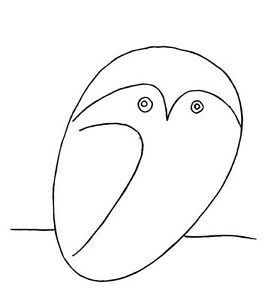
\includegraphics{img/picasso_owl.jpg}
  \caption{Very Basic}
\end{figure}

İlerlemeden önce, Haskell'in kimi temel \st{özelliklerini fark etmeniz}
özelliklerinin bilincine varmanız gerekiyor.

\paragraph{Fonksiyonel}\label{fonksiyonel}

Haskell fonksiyonel bir dildir. İmperatif bir dil geçmişiniz
varsa, bir sürü yeni nes öğrenmeniz gerekiyor. Umarım bu yeni kavramlar
size imperatif dillerde program yazarken bile yardımcı olur.

\paragraph{Akıllı Statik Tip Sistemi}\label{akux131llux131-statik-tip-sistemi}

Tip sistemi, \lstinline!C!'de, \lstinline!C++!'ta, \lstinline!Java!'da
olduğu gibi sizi engellemek yerine size yardım etmek için vardır.

\paragraph{Arılık}\label{saflux131k} % Purity 

Genellikle fonksiyonlarınız dış ortamda bir nesi değiştirmeyecekler. Bu
demek oluyor ki, bir değişkenin değerini değiştiremeyecekler,
kullanıcıdan girdi alamayacaklar, ekrana yazı yazamayacaklar, yada bir
füzeyi ateşleyemeyecekler. Öte %diğer
yandan, paralellik sağlamak çok kolay
olacak. Haskell kodunuzun nerede yan etkileri olduğunun, nerede arı
olduğunun ayrımını çok açık bir biçimde yapar. Ayrıca, programınız
üzerine us yürütmek de çok daha kolay olur. Çoğu yanıl, kodunuzun
yalın bölümünde engellecektir.
% Most bugs will be prevented in the  pure parts of your program.
Daha da ötesi, Haskell'de saf fonksiyonlar temel bir kural izlerler:
\textgreater{} Bir fonksiyona özdeş parametreler vermek hep özdeş
değerleri döndürür.

\paragraph{Üşengeçlik}\label{üsengeclik}

Üşengeçlik, genelde alışılmadık bir dil tasarım seçimidir. Haskell'de
varsayılan işlem olarak her nes yalnızca gereksinim olduğunca işlenir.
%hesaplanır
Bunun sonuçlarından biri, sonsuz yapıları işlemek için çok kusursuz % mükemmel
bir yol sunmasıdır.

Son uyarı da Haskell kodunu hangi yöntemle okumanız gerektiği üzerine. Benim
için, bilimsel anlatıları okumak gibi. Kimi bölümleri çok açık ancak bir
formül gördünüzde odaklanarak yavaşça okuyun. Ayrıca, Haskell
öğrenirken, sıradışı % garip
söz dizimsel (\emph{syntactical}) detayları anlamamanız \emph{gerçekten}
önemli değil. Ancak \lstinline!>>=!, \lstinline!<$>!, \lstinline!<-!
de bunun gibi herhangi bir değişik sembol görürseniz, görmezden gelip kodun
akışını izleyin.

\subsubsection{Fonksiyon tanımı}\label{fonksiyon-tanux131mux131}

Şu biçimde fonksiyon tanımlamaya alışmış olabilirsiniz:

C:

\begin{lstlisting}[language={[ANSI]C},tabsize=2,escapeinside=||]
  int f(int x, int y) {
    return x*x + y*y;
  }
\end{lstlisting}

JavaScript:

\begin{lstlisting}[language=Javascript]
  function f(x,y) {
    return x*x + y*y;
  }
\end{lstlisting}

Python:

\begin{lstlisting}[language=Python]
  def f(x,y):
  return x*x + y*y
\end{lstlisting}

Ruby:

\begin{lstlisting}[language=Ruby]
  def f(x,y)
    x*x + y*y
  end
\end{lstlisting}

Scheme:

\begin{lstlisting}[language=Scheme]
  (define (f x y)
    (+ (* x x) (* y y)))
\end{lstlisting}

Son olarak, Haskell yolu da budur:

\begin{lstlisting}[language=Haskell]
  f x y = x*x + y*y
\end{lstlisting}

Yalın. Parantez yok, \lstinline!def! yok.

Unutmayın, Haskell fonksiyonlar ile tipleri sıkça kullanır. Bu yüzden,
onları tanımlamak oldukça kolaydır. Söz dizimi, gereklilik nedeniyle
özellikle öyle düşünülmüştür.

\subsubsection{Tip örneği}\label{tip-uxf6rneux11fi}

Zorunlu olmasa da, % zorunlu olmamasına rağmen
fonksiyonlar için tip bilgisi genellikle
ayrıca girilir. Zorunlu değildir, çünkü derleyici sizin için çıkarım
yapacak kadar soybağdır.
Yine de tipleri yazmak iyi bir düşüncedir, çünkü
kodun anlaşılmasına yardımcı olur.

Bakalım ne yolla oluyormuş:

\begin{lstlisting}[language=Haskell]
  -- Tipleri belirtmek icin :: imini kullaniyoruz
  f :: Int -> Int -> Int
  f x y = x*x + y*y
  main = print (f 2 3)
\end{lstlisting}

\begin{lstlisting}[language=shell,numbers=none,nolol]
  ~ runhaskell 20_very_basic.lhs
  13
\end{lstlisting}

Şimdi bunu deneyelim:

\begin{lstlisting}[language=Haskell]
  f :: Int -> Int -> Int
  f x y = x*x + y*y
  main = print (f 2.3 4.2)
\end{lstlisting}

Şu yanılı almış olmalısınız:

\begin{lstlisting}[language=shell,numbers=none,nolol]
  21_very_basic.lhs:6:23:
  No instance for (Fractional Int)
  arising from the literal `4.2'
  Possible fix: add an instance declaration for (Fractional Int)
  In the second argument of `f', namely `4.2'
  In the first argument of `print', namely `(f 2.3 4.2)'
  In the expression: print (f 2.3 4.2)
\end{lstlisting}

Sorun şu ki \lstinline!4.2! bir tüm sayı (Int) değil. Çözümü ise: \lstinline!f! fonksiyonu için şimdilik bir tip belirtmeyerek, tip çıkarımını Haskell'e bırakmak.

\begin{lstlisting}[language=Haskell]
  f x y = x*x + y*y
  main = print (f 2.3 4.2)
\end{lstlisting}

Çalışıyor! Ne şanslıyız ki, her tip için yeni bir fonksiyon tanımlamak
zorunda değiliz. Örneğin \lstinline!C!'de, \lstinline!int! için,
\lstinline!float! için, \lstinline!long! için, \lstinline!double! için
de bunun gibi ayrı ayrı fonksiyon tanımlamak zorundayız.

Peki hangi tipi belirtmeliydik? Haskell'in bizim için bulduğu tipi
görmek için \lstinline!ghci!'yi başlatın:

\begin{lstlisting}[language=shell,numbers=none,nolol]
  GHCi, version 7.0.4: http://www.haskell.org/ghc/  :? for help
  Loading package ghc-prim ... linking ... done.
  Loading package integer-gmp ... linking ... done.
  Loading package base ... linking ... done.
  Loading package ffi-1.0 ... linking ... done.
  Prelude> let f x y = x*x + y*y
  Prelude> :type f
  f :: Num a => a -> a -> a
\end{lstlisting}

Ne? Bu değişik tip de neyin nesi?

\begin{lstlisting}[language=Haskell]
  Num a => a -> a -> a
\end{lstlisting}

İlk önce, sağdaki \lstinline!a -> a -> a! bölgesine bakalım. Anlamak için
adım adım ilerleyerek şu örnekleri inceleyelim:

\begin{longtable}[l]{@{}ll@{}} % Bunu hangi an [c] yaptım ? :)
  \toprule
  Yazılı Tip & Anlamı\tabularnewline
  \midrule
  \endhead
  Int & Int tipi\tabularnewline
  Int -\textgreater{} Int & Int'ten Int'e olan fonksiyon
  tipi\tabularnewline
  Float -\textgreater{} Int & Float'tan Int'e olan fonksiyon
  tipi\tabularnewline
  a -\textgreater{} Int & herhangi bir tipten Int'e olan fonksiyon
  tipi\tabularnewline
  a -\textgreater{} a & herhangi bir a tipinden özdeş a tipine olan
  fonksiyon tipi\tabularnewline
  a -\textgreater{} a -\textgreater{} a & herhangi bir a tipinden iki
  argümanın özdeş a tipine olan fonksiyon tipi\tabularnewline
  \bottomrule
\end{longtable}

\lstinline!a -> a -> a! 'da \lstinline!a! imine tip değişkeni
diyoruz. \emph{(type variable)}. Bu \lstinline!f!'nin iki argümanı
olduğu, girilen argümanlar ile fonksiyon sonucunun özdeş tipten olduğu
anlamına geliyor. Tip değişkeni \lstinline!a!, başka bir sürü değer
alabilir. Örneğin \lstinline!Int!, \lstinline!Integer!,
\lstinline!Float!\ldots{}

Dolayısıyla \lstinline!C! 'deki gibi zorunlu olarak bir fonksiyon için
\lstinline!int!, \lstinline!long!, \lstinline!float!, \lstinline!double!
de bunun gibi tip belirtmek yerine, herhangi bir dinamik tip tabanlı dilde
olduğu gibi yalnızca bir fonksiyon tanımlıyoruz.

Buna kimileyin parametrik çokbiçimlilik \emph{(parametric polymorphism)} de
deniyor. Yaşamda her istediğinizin olması gibi bir nes.

Genellikle \lstinline!a! herhangi bir tip olabilir, örneğin
\lstinline!String! yada \lstinline!Int!, ancak \lstinline!Trees! gibi daha
karışık tipler, başka fonksiyonlar da olabilir. Ancak buradaki tipimiz
\lstinline!Num a =>! ile başlıyor.

\lstinline!Num! bir tip klası. \emph{(type class)}. Tip klasları tip
grupları gibi düşünülebilir. \lstinline!Num! klası yalnızca sayı gibi
davranan tipleri içerir. Daha doğrusu, \lstinline!Num!, belli bir
fonksiyon listesinin, özellikle \lstinline!(+)! ve \lstinline!(*)!
fonksiyonlarının, etki ettiği klastır.

Tip sınıfları güçlü bir dil yapısıdır. Onlarla inanılmaz güçlü nesler
yapabiliriz. Buna daha sonra yine değineceğiz.

Sonuç olarak, \lstinline!Num a => a -> a -> a! şu demek oluyor:

Diyelim ki \lstinline!a!, \lstinline!Num! tip klasına ait bir tip. Bu
da \lstinline!a! tipinden \lstinline!a -> a! tipine bir fonksiyon.

Evet, beklenenden değişik. Esasında Haskell'de hiçbir fonksiyonun gerçekten iki
argümanı yoktur. Onun yerine, her fonksiyonun yalnızca bir argümanı
vardır. Ancak anımsamalıyız ki iki argüman almakla, bir argüman alıp
ikinci argümanı bir parametre olarak alan bir fonksiyon döndürmek denk
şeylerdir.

Daha açık olmak gerekirse, \lstinline!f 3 4!, \lstinline!(f 3) 4!'e
denktir. \lstinline!f 3!'un de bir fonksiyon olduğunu gözlemleyin:

\begin{lstlisting}[language=Haskell]
  f :: Num a => a -> a -> a

  g :: Num a => a -> a
  g = f 3

  g y ⇔ 3*3 + y*y
\end{lstlisting}

Fonksiyonlar için bir notasyon daha var. Lambda notasyonu adsız
fonksiyonlar yaratmamıza olanak sağlar. Bunlara anonim fonksiyonlar
diyoruz. Özdeş nesi lambda notasyonu (gösterimi) ile şöyle de yazabilirdik:

\begin{lstlisting}[language=Haskell]
  g = \y -> 3*3 + y*y
\end{lstlisting}

% \begin{verbatim}
Burada \textbackslash{} kullanılıyor, çünkü λ (lambda) imine
benzemekte \st{ve aynı zamanda} olup % eş anlı olarak
ayrıca ASCII dizisinin içindedir.
% \end{verbatim}

Fonksiyonel programlamaya alışık değilseniz beyniniz yanmaya
başlamış olmalı. Artık gerçek bir uygulama yazma anı.

Ancak ondan önce, tip sisteminin beklediğimiz gibi çalıştığını
doğrulayalım:

\begin{lstlisting}[language=Haskell]
  f :: Num a => a -> a -> a
  f x y = x*x + y*y

  main = print (f 3 2.4)
\end{lstlisting}

Çalışıyor, çünkü \lstinline!3! hem \lstinline!Float! gibi rasyonel
\emph{(Fractional)} sayılar için, hem de \lstinline!Integer! (tüm sayı
tipi) için geçerli bir gösterim. \lstinline!2.4! rasyonel bir sayı olduğu
için \lstinline!3! de rasyonel bir sayı olarak yorumlanıyor.

Fonksiyonumuzu birbirinden değişik tiplerle çalışmaya zorlarsak, yanıl
verecektir:

\begin{lstlisting}[language=Haskell]
  f :: Num a => a -> a -> a
  f x y = x*x + y*y

  x :: Int
  x = 3
  y :: Float
  y = 2.4
  main = print (f x y) -- calismayacak, cunku tip x ≠ tip y
\end{lstlisting}

Derleyici yanıl veriyor. İki parametre de özdeş tipten olmak zorunda.

Bunun kötü bir düşünce olduğunu, derleyicinin sizin için bir tipten
ötekine dönüşümü yapması gerektiğini düşünüyorsanız, WAT\footnote{www.destroyallsoftware\centerdot com/talks/wat} adlı korkunç ayrıca komik videoyu \st{mutlaka} kesinlikle izlemelisiniz:

\pagebreak
\section{Temel Haskell}\label{temel-haskell}

\begin{figure}[htbp]
  \centering
  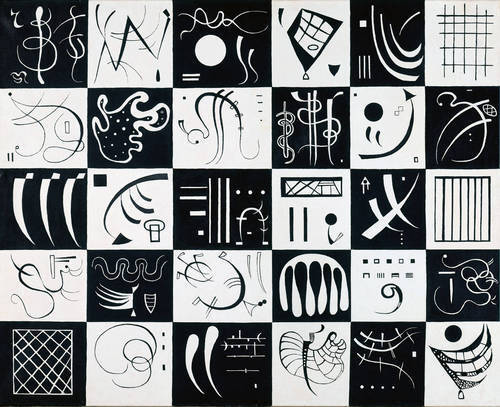
\includegraphics[width=0.6\linewidth]{img/kandinsky_gugg.jpg}
  \caption{Essential}
\end{figure}

Bu bölüme yalnızca göz gezdirmenizi öneriyorum. Her an
yararlanacağınız bir kaynak gibi düşünün. Haskell'in birçok özelliği
vardır. Burada da pek çoğu eksik. Notasyon alışılmadık % garip
gelirse yine buraya dönün.

İki deyimin denk olduğunu belirtmek için $\Leftrightarrow$ imini
kullanıyorum. Bu \st{sahte} yapma notasyon: $\Leftrightarrow$ % ⇔
Haskell'de yoktur.
Özdeş biçimde, bir deyimin \st{hesaplanan} kalküle edilen değerinin ne olduğunu
\st{ifade etmek} belirtmek için de $\Rightarrow$ \st{işaretini} imini kullanacağım.

\subsection{Notasyon}\label{notasyon}

\subsubsection{Aritmetik Notasyon}\label{aritmetik}
% Matematik
% \begin{lstlisting}[language=Haskell] listings paketini kullanamadık
% Çünkü  ⇔ imini gösteremiyor.

\begingroup\Palatino
$$
3 + 2 * 6 / 3 \Leftrightarrow 3 + ((2*6)/3)
$$
\endgroup

\subsubsection{Usbilimsel Notasyon}\label{mantux131ksal}

\begingroup
$$
\Palatino
\begin{aligned}
True\, ||\,   False   &\Rightarrow True\\
True\, \&\&\, False   &\Rightarrow False\\
True\, ==\,   False   &\Rightarrow False\\
True\, /=\,   False   &\Rightarrow True\, (/=)\, esit\, degil\, operatorudur
\end{aligned}
$$
\endgroup

\subsubsection{Üslü Sayılar}\label{uxfcsluxfc-sayux131lar}

\begin{lstlisting}[language=Haskell]
  x^n     herhangi bir n integral tipi icin (Int yada Integer olarak anlayin)
  x**y    herhangi bir y sayi tipi icin (ornegin Float)
\end{lstlisting}

\lstinline!Integer!'ın bilgisayarınızın kapasitesi dışında bir sınırı
yoktur.

\begin{lstlisting}[language=shell,numbers=none,nolol]
  4^103
  102844034832575377634685573909834406561420991602098741459288064
\end{lstlisting}

Evet! Ayrıca rasyonel sayılar da var! Yine de önce \lstinline!Data.Ratio!
modülünü içeri aktarmanız gerekiyor:

\begin{lstlisting}[language=shell,numbers=none,nolol]
  $ ghci
  ....
  Prelude> :m Data.Ratio
  Data.Ratio> (11 \% 15) * (5 % 3)
  11 % 9
\end{lstlisting}

\subsubsection{Listeler}\label{listeler}

\begin{lstlisting}[language=shell,numbers=none,nolol]
  []                      ⇔ bos liste
  [1,2,3]                 ⇔ integral listesi
  ["foo","bar","baz"]     ⇔ String listesi
  1:[2,3]                 ⇔ [1,2,3], (:) bir elemani one ekleme
  1:2:[]                  ⇔ [1,2]
  [1,2] ++ [3,4]          ⇔ [1,2,3,4], (++) birlestirme
  [1,2,3] ++ ["foo"]      ⇔ YANIL! String ≠ Integral
  [1..4]                  ⇔ [1,2,3,4]
  [1,3..10]               ⇔ [1,3,5,7,9]
  [2,3,5,7,11..100]       ⇔ YANIL! O denli soybağ degilim!
  [10,9..1]               ⇔ [10,9,8,7,6,5,4,3,2,1]
\end{lstlisting}

\subsubsection{Karakter Dizileri}\label{karakter-dizileri}

Haskell'de \lstinline!String! tipi, \lstinline!Char! tipinden oluşmuş
listeye denktir.

\begin{lstlisting}
  'a' :: Char
  "a" :: [Char]
  ""    ⇔ []
  "ab"  ⇔ ['a','b'] ⇔  'a':"b" ⇔ 'a':['b'] ⇔ 'a':'b':[]
  "abc" ⇔ "ab"++"c"
\end{lstlisting}

ÖNEMLİ: Gerçek kodda, yazıyı simgelemek üzere \lstinline!Char! listesi
kullanmamalısınız. Genel olarak \lstinline!Data.Text! kullanmalısınız.
ASCII karakter akımını \emph{(stream)} simgelemek istiyorsanız,
onun için de \lstinline!Data.ByteString! kullanmalısınız.

\subsubsection{Demetler \emph{(Tuple)}}\label{demetler-tuple}

Bir ikili demetin tipi \lstinline!(a,b)!'dir. Demetlerdeki elemanlar
birbirinden değişik tipte olabilirler.

\begin{lstlisting}[language=Haskell]
  -- Tum bu demetler gecerlidir
  (2,"foo")
  (3,'a',[2,3])
  ((2,"a"),"c",3)

  fst (x,y)       ⇒  x
  snd (x,y)       ⇒  y

  fst (x,y,z)     ⇒  YANIL: fst :: (a,b) -> a
  snd (x,y,z)     ⇒  YANIL: snd :: (a,b) -> b
\end{lstlisting}

\subsubsection{Parantezlerle Başa
  Çıkmak}\label{parantezlerle-baux15fa-uxe7ux131kmak}

Parantezlerin kimisinden kurtulmak için \lstinline!($)! ile \lstinline!(.)! fonksiyonlarını kullanabilirsiniz.

\begin{lstlisting}[language=Haskell]
  -- Esasinda:
  f g h x         ⇔  (((f g) h) x)

  -- $ imi kendisinden deyimin sonuna
  -- dek olan parantezin yerine gecer
  f g $ h x       ⇔  f g (h x) ⇔ (f g) (h x)
  f $ g h x       ⇔  f (g h x) ⇔ f ((g h) x)
  f $ g $ h x     ⇔  f (g (h x))

  -- (.) kompozisyon fonksiyonu
  (f . g) x       ⇔  f (g x)
  (f . g . h) x   ⇔  f (g (h x))
\end{lstlisting}

\subsection{Fonksiyonlar için Yararlı Notasyonlar}
\label{fonksiyonlar-iuxe7in-yararlux131-notasyonlar}

Anımsatma:

\begin{lstlisting}[language=Haskell]
  x :: Int            ⇔ x Int tipinde herhangi bir deger alabilir
  x :: a              ⇔ x herhangi bir tip olabilir
  x :: Num a => a     ⇔ x Num tip klasi kapsamında olan
  herhangi bir a tipi olabilir
  f :: a -> b         ⇔ f a'dan b'ye bir fonksiyondur
  f :: a -> b -> c    ⇔ f a'dan (b→c)'ye bir fonksiyondur
  f :: (a -> b) -> c  ⇔ f (a→b)'den c'ye bir fonksiyondur
\end{lstlisting}

Bir fonksiyonu tanımlamadan önce tipini belirtmenin zorunlu olmadığını anımsayın.
Haskell genelde tip çıkarımını sizin için kendisi yapar. Ancak
genelde tipleri belirtmek iyi bir pratik olarak görülür.

\paragraph{Orta notasyon}\label{orta-notasyon}

\begin{lstlisting}[language=Haskell]
  square :: Num a => a -> a
  square x = x^2
\end{lstlisting}

\lstinline!^! iminin iç notasyon (\emph{infix notation}) kullandığını özellikle gözlemleyin. Her iç notasyona bağlı bir ön notasyon (\emph{prefix notation}) vardır. O durumda, onu parantez içine koymalısınız.
% For each infix operator there its associated prefix notation. You just have to put it inside parenthesis

\begin{lstlisting}[language=Haskell]
  square' x = (^) x 2

  square'' x = (^2) x
\end{lstlisting}

Soldaki ile sağdaki \lstinline!x!'leri silebiliriz. Buna $η$ (eta)
indirgemesi % Amerika'daki çevirmen yalınlaştırılma, sadeleştirme demiş, yanlış
deniyor.

\begin{lstlisting}[language=Haskell]
  square''' = (^2)
\end{lstlisting}

Değişken adlarında \lstinline!'! kullanabildiğimize özel ilgi gösterin

\lstinline!square! ⇔ \lstinline!square'! ⇔ \lstinline!square''! ⇔
\lstinline!square'''!

\subsubsection{Testler}\label{testler}

Salt değer (\emph{absolute value}) % mutlak
fonksiyonu yazalım:

\begin{lstlisting}[language=Haskell]
  absolute :: (Ord a, Num a) => a -> a
  absolute x = ıf x >= 0 then x else -x
\end{lstlisting}

Özellikle ilgi gösterin  ki Haskell'deki \lstinline!if .. then .. else! notasyonu,
C'deki \lstinline!¤?¤:¤! operatörüne bayağı benzer. \lstinline!else!
bölümünü unutmanız olası değil.

Başka bir denk versiyonu:

\begin{lstlisting}[language=Haskell]
  absolute' x
  | x >= 0 = x
  | otherwise = -x
\end{lstlisting}

Haskell'de paragraf başı ile boşluklar önemlidir. Python'daki gibi, kötü boşluklar kodunuzu bozabilir.

\part{Zor Bölüm}[Zor bölüm şimdi başlıyor.]\label{zor-kux131sux131m}

\section{Fonksiyonel Stil}\label{fonksiyonel-stil}

\begin{figure}[htbp]
  \centering
  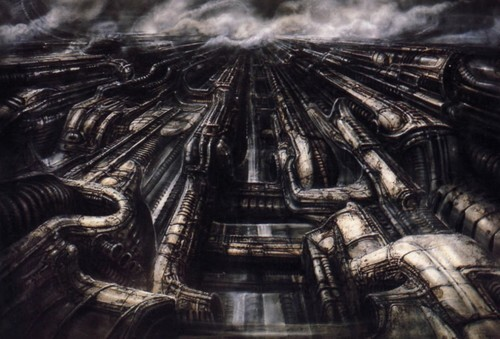
\includegraphics{img/hr_giger_biomechanical_landscape_500.jpg}
  \caption{Functional}
\end{figure}

Bu bölümde, Haskell'in etkileyici yeniden yapılandırma
\emph{(refactoring)} yeteneklerini göreceğiz. Bir problem seçip önce
standart imperatif yolla çözeceğiz. Daha sonra kodu evrimleştireceğiz. 
Son durum hem çok daha elegant % zarif
hem de kolay anlaşılabilir olacak.

% In this section, I will give a short example of the impressive 
% refactoring ability provided by Haskell. We will select a problem and 
% solve it in a standard imperative way. Then I will make the code evolve.
% The end result will be both more elegant and easier to adapt.</p>

Aşağıdaki problemi çözelim:

Verilen bir tüm sayı listesindeki düz (\emph{ikiyle kalansız bölünebilen}) sayıların toplamını alın. Örnek: \lstinline![1,2,3,4,5] ⇒ 2 + 4 ⇒ 6!

Fonksiyonel ile imperatif yaklaşımların arasındaki ayrımı göstermek üzere,
imperatif çözümü göstererek başlayacağım: (JavaScript'te)

\begin{lstlisting}[language=Javascript]
  function evenSum(list) {
    var result = 0;
    for (var i=0; i< list.length ; i++) {
      if (list[i] % 2 ==0) {
      result += list[i];
    }
  }
  return result;
  }
\end{lstlisting}

Haskell'de, öteki dillerden ayrık olarak, değişkenler yada \lstinline!for! döngüleri
yoktur. Döngüler olmaksızın özdeş sonucu elde etmenin bir yolu
özyinel (\emph{recursion})'dir

Önemli: Özyinel, imperatif dillerde genellikle yavaş olarak algılanır.
Fonksiyonel programlamada genellikle durum bu değildir. Çoğu kez % zaman
Haskell özyinel fonksiyonları verimli biçimde işler.

İşte özyinel fonksiyonun C versiyonu. Kolaylık %basitlik
için tüm sayı listesinin ilk \lstinline!0! değeri ile bittiğini
varsaydığımı özellikle gözlemleyin.

\begin{lstlisting}[language= {[ANSI]C},tabsize=2,escapeinside=||]
  int evenSum(int *list) {
    return accumSum(0,list) ;
  }
  int accumSum(int n, int *list) {
  int x;
  int *xs;
  if (*list == 0) { // liste bos ise
    return n;
  }
  else {
    x = list[0]; // x listenin ilk elemani olsun
    xs = list+1; // xs listenin ilk elemani dışında geri kalani olsun
    if ( 0 == (x\%2) ) { // x duz ise
      return accumSum(n+x, xs);
    }
    else {
      return accumSum(n, xs); // Burada sorun var ?
    }
  }
  }
\end{lstlisting}

Bu kodu belleğinizde tutun. Şimdi onu Haskell'e çevireceğiz. Ancak ilk önce,
size burada kullanacağımız üç yalın ancak kullanışlı fonksiyonu tanıtmam
gerekiyor:

\begin{lstlisting}[language=Haskell]
  even :: Integral a => a -> Bool
  head :: [a] -> a
  tail :: [a] -> [a]
\end{lstlisting}

\lstinline!even! bir sayının düz (\emph{ikiyle kalansız bölünebilen}) olduğunu doğrular.

\begin{lstlisting}[language=Haskell]
  even :: Integral a => a -> Bool
  even 3  ⇒ False
  even 2  ⇒ True
\end{lstlisting}

\lstinline!head! bir listenin ilk elemanını döndürür.

\begin{lstlisting}[language=Haskell]
  head :: [a] -> a
  head [1,2,3] ⇒ 1
  head []      ⇒ HATA
\end{lstlisting}

\lstinline!tail! bir listenin ilk elemanı dışında % hariç
tüm elemanlarını döndürür.

\begin{lstlisting}[language=Haskell]
  tail :: [a] -> [a]
  tail [1,2,3] ⇒ [2,3]
  tail [3]     ⇒ []
  tail []      ⇒ HATA
\end{lstlisting}

Görebileceğiniz gibi, herhangi bir boş olmayan \lstinline!l! listesi
için, \lstinline!l ⇔ (head l):(tail l)!

İlk Haskell çözümümüz. \lstinline!evenSum! fonksiyonu bir listedeki tüm
düz sayıların toplamını döndürür.

\begin{lstlisting}[language=Haskell]
  -- Versiyon 1
  evenSum :: [Integer] -> Integer

  evenSum l = accumSum 0 l

  accumSum n l = if l == []
  then n
  else let x = head l
  xs = tail l
  in if even x
  then accumSum (n+x) xs
  else accumSum n xs
\end{lstlisting}

Fonksiyonu denemek için \lstinline!ghci!'ı kullanabilirsiniz.

\begin{lstlisting}
  % ghci
  GHCi, version 7.0.3: http://www.haskell.org/ghc/  :? for help
  Loading package ghc-prim ... linking ... done.
  Loading package integer-gmp ... linking ... done.
  Loading package base ... linking ... done.
  Prelude> :load 11_Functions.lhs
  [1 of 1] Compiling Main             ( 11_Functions.lhs, interpreted )
  Ok, modules loaded: Main.
  *Main> evenSum [1..5]
  6
\end{lstlisting}

Burada çalıştırılma örneğini görebilirsiniz: \footnote{aldatma % hile
  yaptığımı biliyorum. Ancak üşengeçlik konusuna sonra yine değineceğiz.}

\begin{lstlisting}
  *Main> evenSum [1..5]
  accumSum 0 [1,2,3,4,5]
  1 is odd
  accumSum 0 [2,3,4,5]
  2 is even
  accumSum (0+2) [3,4,5]
  3 is odd
  accumSum (0+2) [4,5]
  4 is even
  accumSum (0+2+4) [5]
  5 is odd
  accumSum (0+2+4) []
  l == []
  0+2+4
  0+6
  6
\end{lstlisting}

İmperatif bir dilden geliyorsanız her nes doğru gözüküyor olmalı.
Esasında buradaki pek çok nes geliştirilebilir. Öncelikle, tipi
genelleyebiliriz.

\begin{lstlisting}[language=Haskell]
  evenSum :: Integral a => [a] -> a
\end{lstlisting}

Daha sonra, \lstinline!where! yada \lstinline!let! kullanarak alt
fonksiyonlar tanımlayabiliriz. Bu biçimde  \lstinline!accumSum!
fonksiyonu modülümüzün üst düzey ad uzayını \emph{(namespace)}
kirletmemiş olur.

\begin{lstlisting}[language=Haskell]
  -- Versiyon 2
  evenSum :: Integral a => [a] -> a

  evenSum l = accumSum 0 l
  where accumSum n l =
  if l == []
  then n
  else let x = head l
  xs = tail l
  in if even x
  then accumSum (n+x) xs
  else accumSum n xs
\end{lstlisting}

Sonra, örüntü eşleme \emph{(pattern matching)} kullanabiliriz.

\begin{lstlisting}[language=Haskell]
  -- Versiyon 3
  evenSum l = accumSum 0 l
  where
  accumSum n [] = n
  accumSum n (x:xs) =
  if even x
  then accumSum (n+x) xs
  else accumSum n xs
\end{lstlisting}

Peki örüntü eşleme nedir? Genel parametre adları yerine değerlerin
kendisini kullanın. \footnote{Daha yiğit olanlarınız için örüntü
eşleme üzerine daha kapsamlı bir açıklama 
\href{http://www.cs.auckland.ac.nz/references/haskell/haskell-intro-html/patterns.html}{şuradan}
okunabilir.}

\lstinline!foo l = if l == [] then <x> else <y>! demek yerine, yalnızca
şöyle diyorsunuz:

\begin{lstlisting}[language=Haskell]
  foo [] =  <x>
  foo l  =  <y>
\end{lstlisting}

Ancak örüntü eşleme bundan daha ötesidir. % Aynı anda
% "aynı zamanda" "hem de" "bununla birlikte" "xbaynı anda" "ayrıca"
% "aynı anda" "eş anlı olarak"
Ek olarak
karışık % Amerikalu çevirmen "karmaşık" (messy, complicated) sözcüğü kullanmış
bir değerin iç verisini (\emph{inner data}) yoklamanın bir yoludur
% inspect the inner data of a complex value
Şu kodun yerine:

\begin{lstlisting}[language=Haskell]
  foo l =  let x  = head l
  xs = tail l
  in if even x
  then foo (n+x) xs
  else foo n xs
\end{lstlisting}

şunu yazabiliriz:

\begin{lstlisting}[language=Haskell]
  foo (x:xs) = if even x
  then foo (n+x) xs
  else foo n xs
\end{lstlisting}

Bu çok kullanışlı bir özellik. Ek olarak kodumuzu daha kısa de
okunaklı kılıyor.

Haskell'de $η$-indirgeyerek
% you can simplify function definitions by η-reducing them
fonksiyonları yalınlaştırabilirsiniz. % basitleştirebilirsiniz.
Örneğin, şunu yazmak yerine:

\begin{lstlisting}
  f x = (some expression) x
\end{lstlisting}

basitçe şunu yazabilirsiniz:

\begin{lstlisting}
  f = some expression
\end{lstlisting}

Bu metodu \lstinline!l!'yi kaldirmak icin kullanalim:

\begin{lstlisting}[language=Haskell]
  -- Version 4
  evenSum :: Integral a => [a] -> a

  evenSum = accumSum 0
  where
  accumSum n [] = n
  accumSum n (x:xs) =
  if even x
  then accumSum (n+x) xs
  else accumSum n xs
\end{lstlisting}

% \pagebreak
\subsubsection{Üst Derece Fonksiyonlar}\label{uxfcst-derece-fonksiyonlar}

\begin{figure}[htbp]
  \centering
  
\includegraphics[width=0.5\linewidth]{img/escher_polygon}
  \caption{Higher Order}
\end{figure}

Her şeyi daha da iyi yapmak için, üst derece fonksiyonları
kullanmalıyız. Peki bu canavarlar nelerdir? Üst derece fonksiyonlar,
başka fonksiyonları parametre olarak alan fonksiyonlardır.

\st{Bazı} Kimi örnekleri şöyledir:

\begin{lstlisting}[language=Haskell]
  filter :: (a -> Bool) -> [a] -> [a]
  map :: (a -> b) -> [a] -> [b]
  foldl :: (a -> b -> a) -> a -> [b] -> a
\end{lstlisting}

Ufak adımlarla ilerleyelim.

\begin{lstlisting}[language=Haskell]
  -- Version 5
  evenSum l = mysum 0 (filter even l)
  where
  mysum n [] = n
  mysum n (x:xs) = mysum (n+x) xs
\end{lstlisting}

ki burada,

\begin{lstlisting}[language=Haskell]
  filter even [1..10] ⇔  [2,4,6,8,10]
\end{lstlisting}

\lstinline!filter! fonksiyonu \lstinline!a -> Bool! tipinde bir
fonksiyon ile  \lstinline![a]! tipinde bir listeyi argüman olarak alır.
Bu listeden yalnızca bu fonksiyon çalıştırıldığında \lstinline!True! dönen
elemanları döndürür.

Sonraki adımımız, döngüye benzer bir işlemi başarmak. \lstinline!foldl!
fonksiyonunu listede adım adım ilerlerken yanda bir değer biriktirmek
için kullanacağız. \lstinline!foldl! fonksiyonu esasında şu master yapıyı alıp:

\begin{lstlisting}[language=Haskell]
  myfunc list = foo initialValue list
  foo accumulated []     = accumulated
  foo tmpValue    (x:xs) = foo (bar tmpValue x) xs
\end{lstlisting}

Şu duruma çevirir:

\begin{lstlisting}[language=Haskell]
  myfunc list = foldl bar initialValue list
\end{lstlisting}

Bu gizemli nesnenin gerçekte ne yolla çalıştığını görmek istiyorsanız,
\lstinline!foldl!'in tanımı şöyledir:

\begin{lstlisting}[language=Haskell]
  foldl f z [] = z
  foldl f z (x:xs) = foldl f (f z x) xs
\end{lstlisting}

\begin{lstlisting}[language=Haskell]
  foldl f z [x1,...xn]
  ⇔  f (... (f (f z x1) x2) ...) xn
\end{lstlisting}

Ancak Haskell üşengeç olduğu için \lstinline!(f z x)!'in değerini
bulmadan yalnızca yığının üstüne koyar. Bu yüzden genelde
\lstinline!foldl! yerine \lstinline!foldl'! kullanırız;
\lstinline!foldl'!, \lstinline!foldl! fonksiyonunun üşengeç olmayan
versiyonudur. Üşengeç ile naüşengeç kavramlarını anlamıyorsanız,
tasalanmayın, kodu \lstinline!foldl! ile \lstinline!foldl'! eşit
neslermiş gibi izleyin.

Şimdi \lstinline!evenSum! fonksiyonumuzun yeni durumu şöyle oldu:

\begin{lstlisting}[language=Haskell]
  -- Versiyon 6
  -- foldl' dogrudan erisilebilir
  -- erismek icin once Data.List modulunu iceri almamiz gerekiyor
  import Data.List
  evenSum l = foldl' mysum 0 (filter even l)
  where mysum acc value = acc + value
\end{lstlisting}

Doğrudan lambda notasyonu kullanarak daha da yalınlaştırabiliriz.
Böylece \lstinline!mysum! adında geçici bir fonksiyon yaratmak zorunda
kalmayız.

\begin{lstlisting}[language=Haskell]
  -- Versiyon 7
  -- Genelde yalnızca gerek duydugunuz fonksiyonlari
  -- iceri almak daha iyi bir yontemdir
  import Data.List (foldl')
  evenSum l = foldl' (\x y -> x+y) 0 (filter even l)
\end{lstlisting}

Sonra doğal olarak, özen gösterelim ki:

\begin{lstlisting}[language=Haskell]
  (\x y -> x+y) ⇔ (+)
\end{lstlisting}

Son olarak,

\begin{lstlisting}[language=Haskell]
  -- Versiyon 8
  import Data.List (foldl')
  evenSum :: Integral a => [a] -> a
  evenSum l = foldl' (+) 0 (filter even l)
\end{lstlisting}

\lstinline!foldl'! çok kolay bir fonksiyon sayılmaz. Alışık
değilseniz, üzerinde biraz çalışmalısınız.

Burada ne olup bittiğini görebilmek için \st{kademeli} adım adım ilerleyelim:

\begin{lstlisting}[language=Haskell]
  evenSum [1,2,3,4]
  ⇒ foldl' (+) 0 (filter even [1,2,3,4])
  ⇒ foldl' (+) 0 [2,4]
  ⇒ foldl' (+) (0+2) [4]
  ⇒ foldl' (+) 2 [4]
  ⇒ foldl' (+) (2+4) []
  ⇒ foldl' (+) 6 []
  ⇒ 6
\end{lstlisting}

Başka bir kullanışlı üst derece fonksiyon da \lstinline!(.)!
fonksiyonudur. \lstinline!(.)! fonksiyonu matematiksel bileşimi
\emph{(composition)} anlatır.

\begin{lstlisting}[language=Haskell]
  (f . g . h) x ⇔  f ( g (h x))
\end{lstlisting}

Bu operatörden fonksiyonumuzda $η$ indirgemesi yapmak için
\st{faydanalabiliriz} yararlanabiliriz.

\begin{lstlisting}[language=Haskell]
  -- Versiyon 9
  import Data.List (foldl')
  evenSum :: Integral a => [a] -> a
  evenSum = (foldl' (+) 0) . (filter even)
\end{lstlisting}

Ayrıca, \st{bazı kısımları} kimi bölümleri daha iyi açıklamak için yeniden
\st{isimlendirebiliriz} adlandırabiliriz:

\begin{lstlisting}[language=Haskell]
  -- Versiyon 10
  import Data.List (foldl')
  sum' :: (Num a) => [a] -> a
  sum' = foldl' (+) 0
  evenSum :: Integral a => [a] -> a
  evenSum = sum' . (filter even)
\end{lstlisting}

Şimdi bu fonksiyonel deyimlerle kodumuzun ne yöne doğru gittiğini
tartışalım. Üst derece fonksiyonları kullanmak bize ne kazandırdı?

İlk önce, düşünebilirsiniz ki temel ayrım kısalık. Ancak esasta, ayrım daha
çok doğru düşünmeyle ilgili. Fonksiyonumuzu biraz değiştirmek
istediğimizi varsayalım, örneğin bir listedeki tüm elemanların karesini
alıp o düz kareleri toplamak istediğimizi.

\begin{lstlisting}
  [1,2,3,4] ▷ [1,4,9,16] ▷ [4,16] ▷ 20
\end{lstlisting}

Versiyon 10'u değiştirmek oldukça kolay:

\begin{lstlisting}[language=Haskell]
  squareEvenSum = sum' . (filter even) . (map (^2))
  squareEvenSum' = evenSum . (map (^2))
  squareEvenSum'' = sum' . (map (^2)) . (filter even)
\end{lstlisting}

Yalnızca bir tane daha transformasyon fonksiyonu ekledik, \st{o kadar} hepsi bu.
\footnote{\lstinline!squareEvenSum''! fonksiyonunun öteki ikisinden daha
  verimli olduğuna \st{dikkat edin} özellikle ilgi gösterin \lstinline!(.)! fonksiyonunun sırası
  önemlidir.}

\begin{lstlisting}[language=Haskell]
  map (^2) [1,2,3,4] ⇔ [1,4,9,16]
\end{lstlisting}

\lstinline!map! fonksiyonu \st{basitçe} açıkça bir listenin tüm elemanlarını
etkiler.

Fonksiyon tanımının \emph{içinde} herhangi bir \st{şey} nes değiştirmek zorunda
kalmadık. Ancak ek olarak, fonksiyonunuz \st{hakkında} üzerine daha matematiksel olarak
\st{akıl} us yürütebiliyorsunuz. Ayrıca fonksiyonunuzu ötekileriyle değişmeli kullanabiliyorsunuz.
Dolayısıyla, yeni fonksiyonunuzu kullanarak
\lstinline!compose!, \lstinline!map!, \lstinline!fold!,
\lstinline!filter! işlemlerini yapabilirsiniz.

Versiyon 1'i değiştirmek de okura bir alıştırma olarak kalsın \emoji{slightly-smiling-face} % ☺

Genellemenin sonuna geldiğimizi düşünüyorsanız, oldukça
yanılıyorsunuz. Örneğin, bunu yalnızca liste değil başka herhangi bir
özyinelemeli türde kullanmanın yolları var. Ne yolla olduğunu bilmek
istiyorsanız, size şu eğlenceli \st{makaleyi} anlatıyı okumanızı öneririm:
{\color{blue}Muz, Mercek, Zarf, Dikenli Tellerle Fonksiyonel Programlama - Meijer, Fokkinga, Paterson}
\footnote{eprints.eemcs.utwente\centerdot nl/7281/01/db-utwente-40501F46.pdf}

Bu örnek size arı fonksiyonel programlamanın ne denli güzel olduğunu
göstermeli. Ne yazık ki, arı fonksiyonel programlama her kullanıma tam
uygun değil. Ya da en azından öyle bir programlama dili şu ana dek yok.

Haskell'in büyük güçlerinden biri de alana özel dil \emph{(domain specific language)}
yaratma yeteneğidir, böylece programlama paradigmasını (\emph{yaklaşımını})
değiştirebilirsiniz.

Esasında, Haskell imperatif stilde program yazmak istediğinizde de
güzeldir. İlk Haskell öğrenmeye başladığımda bunu anlamak oldukça zor
olmuştu. Genelde herkes fonksiyonel yaklaşımın üstünlüğünü anlatmaya
çalışır. Daha sonra Haskell'le imperatif stil kullanmaya başlayınca,
ne yolla, hangi anda öyle olacağını anlamak zor olabiliyor.

Bu Haskell süper gücüyle ilgili konuşmadan önce, Haskell'in başka bir
temel yönün\st{den bahsetmeliyiz} e değinmeliyiz: Tipler.


\pagebreak
\section{Tipler}\label{tipler}
\begin{figure}[htbp]
  \centering
  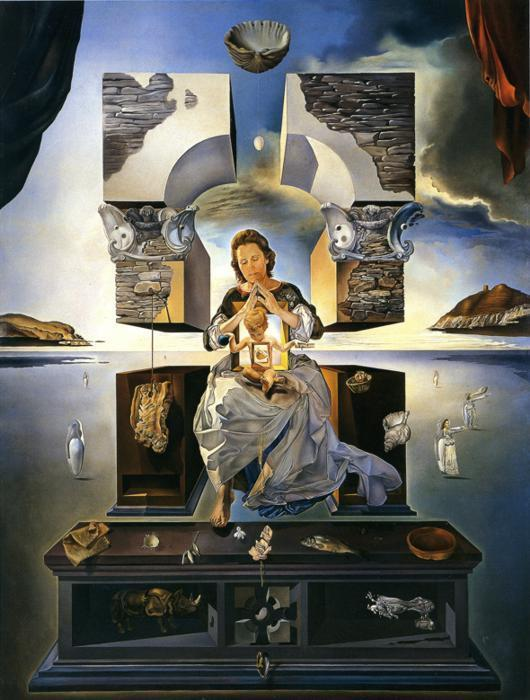
\includegraphics{img/salvador-dali-the-madonna-of-port-lligat.jpg}
  \caption{Types}
\end{figure}

TL, DR (Çok uzundu okumadım):
\begin{itemize}
  \item \lstinline!type Ad = BaskaTip! yalnızca bir takma \st{addır ve} ad olup derleyici \lstinline!Ad! ile \lstinline!BaskaTip!
    arasında bir ayrım gözetmez.
  \item \lstinline!data Ad = AdYapısı BaskaTip! yapısında ayrım vardır.
  \item \lstinline!data! anahtar sözcüğü özyinelemeli yapılar yaratabilir.
  \item \lstinline!deriving! gizemlidir, sizin için fonksiyonlar yaratır.
\end{itemize}

Haskell'de tipler \st{güçlü ve statiktir} hem güçlü hem statiktir.

Peki bu neden önemli? Çünkü bu, yanıllardan kaçınmanıza \emph{yüksek
  derecede} yardımcı olur. Haskell'de yanılların çoğu derleme
aşamasında yakalanır. Bunun asıl nedeni de tip çıkarımının derleme
sırasında yapılmasıdır. Örneğin tip çıkarımı hangi yanlış parametreyi
hangi yerde kullandığınızı yakalar.

\subsubsection{Tip Çıkarımı}\label{tip-uxe7ux131karux131mux131}

Statik tip sistemi hızlı çalıştırma için genelde önemlidir. Ancak çoğu
statik tip sistemli diller kavramları genellemede kötüdür. Haskell'in
kurtarıcı \st{lütfü} yanı, tipleri kendi kendine \emph{çıkarım} yaparak
bulabilmesidir.

Yalın bir örnekle başlayalım, Haskell'deki \lstinline!square!
fonksiyonu:

\begin{lstlisting}[language=Haskell]
  square x = x * x
\end{lstlisting}

\lstinline!square! fonksiyonu Haskell'deki herhangi bir sayısal değerin
karesini alabilir. \lstinline!square! fonksiyonuna parametre olarak
\lstinline!Int!, \lstinline!Integer!, \lstinline!Float!,
\lstinline!Fractional!, hatta \lstinline!Complex! tipinde veri bile
verebilirsiniz. Örnekle kanıtlayalım:

\begin{lstlisting}
  % ghci
  GHCi, version 7.0.4:
  ...
  Prelude> let square x = x*x
  Prelude> square 2
  4
  Prelude> square 2.1
  4.41
  Prelude> -- load the Data.Complex module
  Prelude> :m Data.Complex
  Prelude Data.Complex> square (2 :+ 1)
  3.0 :+ 4.0
\end{lstlisting}

\lstinline!x :+ y! kompleks sayıların gösteriminde kullanılır. (x + iy)

Şimdi C'deki gerekli kod \st{miktarıyla} niceliği ile karşılaştıralım:

\begin{lstlisting}[language= {[ANSI]C},tabsize=2,escapeinside=||]
  int int\_square(int x) { return x * x; }
  float float\_square(float x) {return x * x; }
  complex complex\_square (complex z) {
    complex tmp;
    tmp.real = z.real * z.real - z.img * z.img;
    tmp.img = 2 * z.img * z.real;
  }
  complex x,y;
  y = complex\_square(x);
\end{lstlisting}

C'de her tip için yeni bir fonksiyon yazmanız gerekiyor. Bunu aşmanın
tek yolu ön-işlemciyi (\emph{pre-processor}) kullanarak üst-programlama \st{hilelerine} yöntemlerine başvurmak.
C++'ta daha iyi bir yol var, C++ şablonları:

\begin{lstlisting}[language= {[ANSI]C++},tabsize=2,escapeinside=||]
  #include <iostream>
  #include <complex>
  using namespace std;

  template<typename T>
  T square(T x)
  {
    return x*x;
  }

  int main() {
    // int
    int sqr\_of\_five = square(5);
    cout << sqr\_of\_five << endl;
    // double
    cout << (double)square(5.3) << endl;
    // complex
    cout << square(complex<double>(5,3) )
    << endl;
    return 0;
  }
\end{lstlisting}

C++ bu yönden C'den çok daha iyi iş çıkartıyor. Ancak daha karmaşık
fonksiyonlar için söz dizimini izlemek biraz daha zor olabilir:
örnek için
{\color{blue} what does haskell have to do with c}\footnote{bartoszmilewski\centerdot com/2009/10/21/what-does-haskell-have-to-do-with-c} bakabilirsiniz.

C++'ta bir fonksiyonun \st{farklı} değişik tiplerle çalışacağını ayrıca
belirtmelisiniz. Haskell'de durum tam tersi. Fonksiyon varsayılan olarak
olabildiğince genel tanımlanır.

Tip çıkarımı Haskell'de dinamik tip sistemli dillerin yarattığı özgürlük
\st{hissini} duygusunu yaratır. Ancak dinamik tip sistemli dillerden \st{farklı} ayrı olarak çoğu yanıl, çalışma \st{zamanından} anından önce yakalanır. Genelde Haskell kodu
\textgreater{} derleniyorsa, \st{mutlaka} salt \st{kastettiğiniz} amaçladığınız \st{şeyi} işi yapıyordur.

\subsubsection{Tip Oluşturma \emph{Type construction}}\label{tip-oluux15fturma}

Kendi tiplerinizi oluşturabilirsiniz. İlk önce takma adlarla (\emph{aliases}), dolayısıyla tip
eşanlamlılarıyla (\emph{synonyms}) başlayalım.

\emph{\small You can construct your own types. First, you can use aliases or type synonyms.}

\begin{lstlisting}[language=Haskell]
  type Name   = String
  type Color  = String

  showInfos :: Name ->  Color -> String
  showInfos name color =  "Ad: " ++ name
  ++ ", Renk: " ++ color
  name :: Name
  name = "Erkan"
  color :: Color
  color = "Mavi"
  main = putStrLn $ showInfos name color
\end{lstlisting}

Ancak bu \st{çok fazla} yeterli koruma \st{yaratmıyor} sağlamıyor. \lstinline!showInfos! fonksiyonuna verdiğiniz parametrelerin yerini değiştirip çalıştırmayı deneyin:

\begin{lstlisting}
  putStrLn $ showInfos color name
\end{lstlisting}

Derlenecek \st{ve}, çalışacak. \st{Aslında} Esasında, \lstinline!Name!, \lstinline!Color! \st{ve} ile
\lstinline!String! tiplerini birbiriyle değiştirebilirsiniz, bir \st{fark} ayrım
yaratmayacak. Derleyici hepsine \st{aynıymış} eşitmiş gibi \st{muamele edecek} davranacak.

\st{Diğer} Başka bir yöntem de \lstinline!data! anahtar \st{kelimesini} sözcüğünü kullanarak kendi tiplerinizi yaratmak.

\begin{lstlisting}[language=Haskell]
  data Name   = NameConstr String --NameConstr : ad yapici
  data Color  = ColorConstr String --ColorConstr : renk yapici

  showInfos :: Name ->  Color -> String
  showInfos (NameConstr name) (ColorConstr color) =
  "Name: " ++ name ++ ", Color: " ++ color

  name  = NameConstr "Erkan"
  color = ColorConstr "Mavi"
  main = putStrLn $ showInfos name color
\end{lstlisting}

Ancak şimdi \lstinline!showInfos! için parametrelerin yerlerini
değiştirirseniz, derleyici yanıl verecek! Dolayısıyla bu bir daha yapmayacağınız
\st{muhtemel} olası bir hata \st{ve} olup kaçınmak için tek yapmanız gereken biraz daha uzun yazmak.

Yapıcıların da birer fonksiyon olduğuna \st{dikkat edin} özellikle bakın:

\begin{lstlisting}[language=Haskell]
  NameConstr  :: String -> Name
  ColorConstr :: String -> Color
\end{lstlisting}

\lstinline!data! anahtar sözcüğünün genel söz dizimi de şöyledir:

\begin{lstlisting}[language=Haskell]
  data TipAdi =   YapiciAdi  [tipler]
  | YapiciAdi2 [tipler]
  | ...
\end{lstlisting}

Genel kullanım tip adı ile yapıcı adının \st{aynı} özdeş olması yönündedir.

Örnek:

\begin{lstlisting}[language=Haskell]
  data Complex = Num a => Complex a a
\end{lstlisting}

\st{Kayıt} Kütük \emph{(record)} söz dizimini de kullanabilirsiniz:

\begin{lstlisting}[language=Haskell]
  data VeriTipiAdi = VeriYapicisi {
    alan_1 :: [alan_1 tipi]
    , alan_2 :: [alan_2 tipi]
    ...
    , alan_n :: [alan_n tipi] }
\end{lstlisting}

Daha da iyisi, alanlara erişim sağlayan fonksiyonlar sizin için
oluşturuluyor. Ayrıca bu tipte bir veri oluştururken alanların sırasını
da kullanabilirsiniz.

Örnek:

\begin{lstlisting}[language=Haskell]
  data Complex = Num a => Complex { real :: a, img :: a}
  c = Complex 1.0 2.0
  z = Complex { real = 3, img = 4 }
  real c ⇒ 1.0
  img z ⇒ 4
\end{lstlisting}

\subsubsection{\texorpdfstring{Özyinelemeli Tipler
    \emph{(Recursive
      types)}}{3.2.3. Özyinelemeli Tipler (Recursive types)}}\label{uxf6zyinelemeli-tipler-recursive-types}

Daha önce özyinelemeli bir tiple karşılaşmıştık: listeler. Liste tipini
-biraz daha uzun bir söz dizimiyle de olsa- kendimiz de oluşturabiliriz:

\begin{lstlisting}[language=Haskell]
  data List a = Empty | Cons a (List a)
\end{lstlisting}

\st{Eğer} Daha kolay bir söz dizimi yaratmak istiyorsanız, yapıcılar için iç
notasyon \emph{(infix)} tanımlayabilirsiniz.

\begin{lstlisting}[language=Haskell]
  infixr 5 :::
  data List a = Nil | a ::: (List a)
\end{lstlisting}

\lstinline!infixr!'dan sonraki sayı önceliği belirtiyor.

Bu veri tipini ekrana yazdırmak (\lstinline!Show!), karakter
dizisinden çevirmek (\lstinline!Read!), eşitliğini test edip
(\lstinline!Eq!)  karşılaştırmak (\lstinline!Ord!) istiyorsanız,
Haskell'e sizin için gerekli fonksiyonları oluşturmasını
söyleyebilirsiniz.

\begin{lstlisting}[language=Haskell]
  infixr 5 :::
  data List a = Nil | a ::: (List a)
  deriving (Show,Read,Eq,Ord)
\end{lstlisting}

Veri tipi tanımınıza \lstinline!deriving (Show)!'u eklediğinizde,
Haskell sizin için bir \lstinline!show! fonksiyonu yaratır.
(\emph{(deriving)} İngilizce'de \st{türeme} \emph{türetme} demektir.) Yakında kendi
\lstinline!show! fonksiyonunuzu \st{nasıl} ne biçimde kullanabileceğinizi göreceğiz.

\begin{lstlisting}[language=Haskell]
  convertList [] = Nil
  convertList (x:xs) = x ::: convertList xs

  main = do
  print (0 ::: 1 ::: Nil)
  print (convertList [0,1])
\end{lstlisting}

Bu şu çıktıyı verir:

\begin{lstlisting}
  0 ::: (1 ::: Nil)
  0 ::: (1 ::: Nil)
\end{lstlisting}

\subsubsection{Ağaçlar}\label{aux11fauxe7lar}

\begin{figure}[htbp]
  \centering
  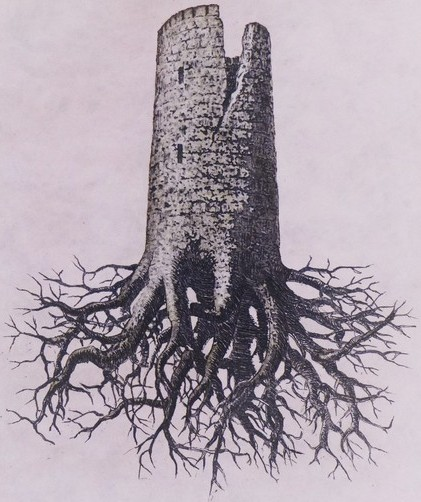
\includegraphics[width=0.5\linewidth]{img/magritte-l-arbre.jpg}
  \caption{Trees}
\end{figure}

Başka bir standart örnek verelim: ikili ağaçlar.

\begin{lstlisting}[language=Haskell]
  import Data.List

  data BinTree a = Empty
  | Node a (BinTree a) (BinTree a)
  deriving (Show)
\end{lstlisting}

Şimdi de bir listeyi sıralı bir ikili ağaca dönüştüren bir fonksiyon
yazalım:

\begin{lstlisting}[language=Haskell]
  treeFromList :: (Ord a) => [a] -> BinTree a
  treeFromList [] = Empty
  treeFromList (x:xs) = Node x (treeFromList (filter (<x) xs))
  (treeFromList (filter (>x) xs))
\end{lstlisting}

Fonksiyonun ne \st{kadar} denli okunaklı olduğunu görebiliyor musunuz?
Düz Türkçe olarak yazarsak: * boş liste, boş ağaca çevrilir. * bir liste
\lstinline!(x:xs)!, bir ağaca çevrilir ki, * kok \lstinline!x!'tır. *
sol alt ağaç, \lstinline!xs!'in \lstinline!x!'ten kesin olarak küçük
elemanlarından oluşturulur. * sağ alt ağaç, \lstinline!xs!'in
\lstinline!x!'ten kesin olarak büyük elemanlarından oluşturulur.

\begin{lstlisting}[language=Haskell]
  main = print $ treeFromList [7,2,4,8]
\end{lstlisting}

Şu sonucu alıyor olmalısınız:

\begin{lstlisting}[language=Haskell]
  Node 7 (Node 2 Empty (Node 4 Empty Empty))\\
  (Node 8 Empty Empty)
\end{lstlisting}

Bu ağacımızın düzgün ancak zor anlaşılır bir \st{temsili} sembolik notasyonu.

Ağacımız için daha iyi bir gösterim kodu, öylesine yazalım. Ben genel
olarak ağaçları daha iyi göstermek için bir fonksiyon yazarken eğlendim,
\st{eğer bu kısmı takip etmeyi} bu bölümü izlemeyi zor buluyorsanız atlayabilirsiniz, bir sorun olmaz.

Değiştirmemiz gereken kimi nesler var. \lstinline!BinTree! tipımizden
\lstinline!deriving (Show)! \st{kısmını}  bölümünü kaldırıyoruz. Ayrıca, BinTree
tipimizi (\lstinline!Eq! ve \lstinline!Ord!)'un \st{sınıflarından} klaslarından türetmek,
eşitlik \st{ve} de karşılaştırma testleri yapmamızı sağlayacaktır.

\begin{lstlisting}[language=Haskell]
  data BinTree a = Empty
  | Node a (BinTree a) (BinTree a)
  deriving (Eq,Ord)
\end{lstlisting}

\lstinline!deriving (Show)! bölümü olmadan Haskell sizin için bir
\lstinline!show! metodu \st{yaratmaz} oluşturma. Biz \lstinline!show! metodu için kendi
versiyonumuzu yazacağız. Bunu başarmak için, yeni oluşturduğumuz
\lstinline!BinTree a!'nin \lstinline!Show! tip klasının bir üyesi
olduğunu belirtmemiz gerekiyor. Bunun için genel söz dizimi şöyle:

\begin{lstlisting}[language=Haskell]
  instance Show (BinTree a) where
  show t = ... -- burada kendi fonksiyonunuzu tanimliyorsunuz
\end{lstlisting}

Benim bir ikili ağacı göstermek için yazdığım versiyon aşağıda.
Karmaşıkmış gibi görünüyor ancak \st{endişelenmeyin} kaygılanmayın.
Daha \st{garip} sıradışı nesneleri de göstermesi için \st{bazı}
birkaç iyileştirme\st{ler} yaptım.

\begin{lstlisting}[language=Haskell]
  -- BinTree'a nin Show tip klasına uye oldugunu belirtin
  instance (Show a) => Show (BinTree a) where
  -- kokten once bir '<' ile baslayacagiz
  -- satir basina da : koyacagiz
  show t = "< " ++ replace '\n' "\n: " (treeshow "" t)
  where
  -- treeshow pref Tree
  --   bu fonksiyon her kod sırasına pref ile baslayarak
  bir agaci gosterecek
  -- Bos agaci gostermeyecek
  treeshow pref Empty = ""
  -- Yaprak
  treeshow pref (Node x Empty Empty) =
  (pshow pref x)

  -- Sag alt agac bos
  treeshow pref (Node x left Empty) =
  (pshow pref x) ++ "\n" ++
  (showSon pref "`--" "   " left)

  -- Sol alt agac bos
  treeshow pref (Node x Empty right) =
  (pshow pref x) ++ "\n" ++
  (showSon pref "`--" "   " right)

  -- Sol ile sag alt agaclari bos olmayan agac
  treeshow pref (Node x left right) =
  (pshow pref x) ++ "\n" ++
  (showSon pref "|--" "|  " left) ++ "\n" ++
  (showSon pref "`--" "   " right)

  -- Agaci guzel gostermek icin on ekler kullan
  showSon pref before next t =
  pref ++ before ++ treeshow (pref ++ next) t

  -- pshow "\n"'i' "\n"++pref ile degistiriyor
  pshow pref x = replace '\n' ("\n"++pref) (show x)

  -- bir karakteri öteki karakter dizisi ile degistiriyor
  replace c new string =
  concatMap (change c new) string
  where
  change c new x
  | x == c = new
  | otherwise = x:[] -- "x"
\end{lstlisting}

\lstinline!treeFromList! metodu \st{tamamen aynı} hiç değişmeden kalıyor.

Şimdi, görelim \st{nasıl} ne yolla oluyormuş:

\begin{lstlisting}[language=Haskell]
  main = do
  putStrLn "Tum sayi ikili agaci:"
  print $ treeFromList [7,2,4,8,1,3,6,21,12,23]
\end{lstlisting}

\begin{lstlisting}
  Tum sayi ikili agaci:
  < 7
  : |--2
  : |  |--1
  : |  `--4
  : |     |--3
  : |     `--6
  : `--8
  :    `--21
  :       |--12
  :       `--23
\end{lstlisting}

Çok daha iyi değil mi? Ağacın kökü \lstinline!<! karakteriyle başlayan
\st{satırda} kod sırasında gösteriliyor. İzleyen her kod \lstinline!:! imi ile
başlıyor. Ağacımızda başka tiplerde veri de kullanabilirdik.

\begin{lstlisting}[language=Haskell]
  putStrLn "\nKarakter dizisi ikili agaci:"
  print $ treeFromList ["foo","bar","baz","gor","yog"]
\end{lstlisting}

\begin{lstlisting}
  Karakter dizisi ikili agaci:
  < "foo"
  : |--"bar"
  : |  `--"baz"
  : `--"gor"
  :    `--"yog"
\end{lstlisting}

Ağaçların eşitliği ile büyük/küçüklüğünü test edebildiğimiz için,
ağaçlardan ağaç da yapabiliriz!

\begin{lstlisting}[language=Haskell]
  putStrLn "\nKarakter ikili agaclarinin ikili agaci:"
  print ( treeFromList
  (map treeFromList ["baz","zara","bar"]))
\end{lstlisting}

\begin{lstlisting}
  Karakter ikili agaclarinin ikili agaci:
  < < 'b'
  : : |--'a'
  : : `--'z'
  : |--< 'b'
  : |  : |--'a'
  : |  : `--'r'
  : `--< 'z'
  :    : `--'a'
  :    :    `--'r'
\end{lstlisting}

Ağacın her \st{satırını} kod sırasını bu yüzden \lstinline!:! ile başlatmıştım.
(kök \st{hariç} dışında)

\begin{figure}[htbp]
  \centering
  
\includegraphics{img/yo_dawg_tree.jpg}
  \caption{Yo}
\end{figure}

\begin{lstlisting}[language=Haskell]
  putStrLn "\nKarakter ikili agaclarinin ikili agaci:"
  print $ (treeFromList . map (treeFromList . map treeFromList))
  [ ["YO","DAWG"]
    , ["I","HEARD"]
    , ["I","HEARD"]
    , ["YOU","LIKE","TREES"] ]
\end{lstlisting}

ki bu da şuna denk (\emph{equivalent},``eşdeğer''):

\begin{lstlisting}[language=Haskell]
  print ( treeFromList (
  map treeFromList
  [ map treeFromList ["YO","DAWG"]
    , map treeFromList ["I","HEARD"]
    , map treeFromList ["I","HEARD"]
    , map treeFromList ["YOU","LIKE","TREES"] ]))
\end{lstlisting}

\st{ve} şu çıktıyı vermeli:

\begin{lstlisting}
  Karakter ikili agaclarinin ikili agaci:
  < < < 'Y'
  : : : `--'O'
  : : `--< 'D'
  : :    : |--'A'
  : :    : `--'W'
  : :    :    `--'G'
  : |--< < 'I'
  : |  : `--< 'H'
  : |  :    : |--'E'
  : |  :    : |  `--'A'
  : |  :    : |     `--'D'
  : |  :    : `--'R'
  : `--< < 'Y'
  :    : : `--'O'
  :    : :    `--'U'
  :    : `--< 'L'
  :    :    : `--'I'
  :    :    :    |--'E'
  :    :    :    `--'K'
  :    :    `--< 'T'
  :    :       : `--'R'
  :    :       :    |--'E'
  :    :       :    `--'S'
\end{lstlisting}

\st{Tekrar edilen} Yinelenen ağaçların eklenmediğine \st{dikkat edin} özen gösterin;
\lstinline!"I","HEARD"!'e denk gelen yalnızca bir ağaç var. Bunun için
(neredeyse) hiçbir \st{şey} nes yapmadık çünkü Tree yapısını \lstinline!Eq! tip
klasından türettik.

Bu yapının ne \st{kadar} denli \st{müthiş} iyi olduğunu görebiliyor musunuz: Yalnızca
sayılardan, karakter dizilerinden, karakterlerden değil, başka
ağaçlardan da ağaçlar yapabiliyoruz. İstersek ağaçlardan oluşan
ağaçlardan oluşan ağaç bile yapabiliriz!

\section{Sonsuz Yapılar}\label{sonsuz-yapux131lar}

\begin{figure}[htbp]
  \centering
  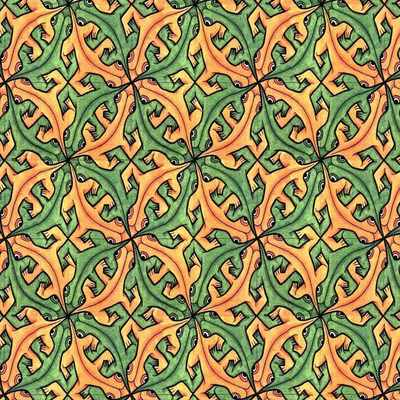
\includegraphics[width=0.4\linewidth]{img/escher_infinite_lizards.jpg}
  \caption{Infinite}
\end{figure}

Haskell'in \emph{üşengeç} olduğu sıkça söylenir. \st{Aslında} Esasında \st{eğer} biraz titizseniz, Haskell'in
{\color{blue}non-strict}\footnote{www.haskell.org/haskellwiki/Lazy\_vs.\_non-strict}
(\st{aceleci olmayan} hemen işlem yapmayan, kesin olmayan) olduğunu söylemelisiniz. Üşengeçlik
yalnızca \emph{non-strict} dillerin ortak bir \st{tatbikidir} uygulamasıdır. Öyleyse ``non-strict'' \st{tam olarak} net biçimde ne anlama geliyor? Haskell vikisiden alıntılayalım:

\st{Sadeleştirme} Yalınlaştırma (\st{hesaplama} kalkülasyon için matematiksel terim) dıştan içe doğru ilerler. \st{yani} dolayısıyla \st{eğer} \lstinline!(a+(b*c))!'yi ele alıyorsanız, önce \lstinline!+!'yi yalınlaştırır, sonra iç \lstinline!(b*c)!'yi  yalınlaştırırsınız.

Örneğin Haskell'de şunu yapabilirsiniz:

\begin{lstlisting}[language=Haskell]
  -- numbers = [1,2,..]
  numbers :: [Integer]
  numbers = 0:map (1+) numbers

  take' n [] = []
  take' 0 l = []
  take' n (x:xs) = x:take' (n-1) xs

  main = print $ take' 10 numbers
\end{lstlisting}

Sonra duruyor. Neden?

\lstinline!numbers! değişkeninin \st{tamamını} tümünü \st{hesaplamak} kalküle etmek yerine, yalnızca
\st{ihtiyacı} gereksinimi olan elemanları, \st{ihtiyacı} gereksinimi \st{olduğu zaman} olduğunda kalküllüyor.

Ayrıca, Haskell'de sonsuz listeler için bir notasyon olduğunu da
söylemiş olayım:

\begin{lstlisting}[language=Haskell]
  [1..]   ⇔ [1,2,3,4...]
  [1,3..] ⇔ [1,3,5,7,9,11...]
\end{lstlisting}

\st{ve} ayrıca çoğu fonksiyon da onlarla çalışır. Ek olarak, Haskell'de, bizim
\lstinline!take'! fonksiyonumuza denk bir \lstinline!take! fonksiyonu
\st{mevcuttur} vardır.


Sıralı ikili ağaç yaptığımızı varsayalım. Sonsuz bir ikili ağaç şöyle
olur:

\begin{lstlisting}[language=Haskell]
  nullTree = Node 0 nullTree nullTree
\end{lstlisting}

Her düğümün 0'a eşit olduğu, geçerli, \st{tam} bütün bir ikili ağaç. Şimdi bu
objeyi aşağıdaki fonksiyonla işleyebileceğimi kanıtlayacağım:

\begin{lstlisting}[language=Haskell]
  -- bir BinTree'nin tum elemanlarini
  -- belli bir derinlige dek al
  treeTakeDepth _ Empty = Empty
  treeTakeDepth 0 _     = Empty
  treeTakeDepth n (Node x left right) = let
  nl = treeTakeDepth (n-1) left
  nr = treeTakeDepth (n-1) right
  in
  Node x nl nr
\end{lstlisting}

Bu programın sonucunu görelim.

\begin{lstlisting}[language=Haskell]
  main = print $ treeTakeDepth 4 nullTree
\end{lstlisting}

Kodumuz derleniyor, \st{çalışıyor ve} çalışıp şu sonucu vererek duruyor:

\begin{lstlisting}
  <  0
  : |-- 0
  : |  |-- 0
  : |  |  |-- 0
  : |  |  `-- 0
  : |  `-- 0
  : |     |-- 0
  : |     `-- 0
  : `-- 0
  :    |-- 0
  :    |  |-- 0
  :    |  `-- 0
  :    `-- 0
  :       |-- 0
  :       `-- 0
\end{lstlisting}

Nöronlarınızı biraz daha ısındırmak için daha ilginç bir ağaca bakalım:

\begin{lstlisting}[language=Haskell]
  iTree = Node 0 (dec iTree) (inc iTree)
  where
  dec (Node x l r) = Node (x-1) (dec l) (dec r)
  inc (Node x l r) = Node (x+1) (inc l) (inc r)
\end{lstlisting}

Bu ağacı oluşturmanın başka bir yolu da üst derece fonksiyonları
kullanmaktır. Bu fonksiyon \lstinline!map! fonksiyonuna benziyor, ancak
listeler yerine \lstinline!BinTree!'ler üzerinde çalışıyor. Ortaya şöyle
bir fonksiyon çıkacak:

\begin{lstlisting}[language=Haskell]
  -- bir fonksiyonu agacin her dugumune uygular
  treeMap :: (a -> b) -> BinTree a -> BinTree b
  treeMap f Empty = Empty
  treeMap f (Node x left right) = Node (f x)
  (treeMap f left)
  (treeMap f right)
\end{lstlisting}

\emph{Not:} Bunun \st{hakkında} üzerine burada daha \st{fazla} öte konuşmayacağım.
\st{Eğer} \lstinline!map!'in öteki veri yapılarına genellemesiyle
ilgileniyorsanız, \emph{functor}ları \st{ve} ile \lstinline!fmap!'i araştırın.

Şimdi tanımımız şöyle oldu:

\begin{lstlisting}[language=Haskell]
  infTreeTwo :: BinTree Int
  infTreeTwo = Node 0 (treeMap (\x -> x-1) infTreeTwo)
  (treeMap (\x -> x+1) infTreeTwo)
\end{lstlisting}

Şunun sonucuna bakalım:

\begin{lstlisting}[language=Haskell]
  main = print $ treeTakeDepth 4 infTreeTwo
\end{lstlisting}

\begin{lstlisting}
  <  0
  : |-- -1
  : |  |-- -2
  : |  |  |-- -3
  : |  |  `-- -1
  : |  `-- 0
  : |     |-- -1
  : |     `-- 1
  : `-- 1
  :    |-- 0
  :    |  |-- -1
  :    |  `-- 1
  :    `-- 2
  :       |-- 1
  :       `-- 3
\end{lstlisting}


\part{Çok Zor Bölüm}\label{uxe7ok-zor-kux131sux131m}

Buraya \st{kadar} geldiyseniz kutlamalar! Şimdi gerçekten çok zor \st{kısım}
 bölüm başlayabilir.

\st{Eğer} Benim gibiyseniz, fonksiyonel stili anlamış olmalısınız. Ayrıca
üşengeçliğin \st{varsayılan} bir norm olmasının avantajlarını da biraz anlamış
olmalısınız. Ancak gerçek bir program yapmaya nereden başlamanız
gerektiğini bilmiyorsunuz. Özellikle de şu soruların \st{cevaplarını} yanıtlarını:
\begin{itemize}
\item Yan etkilerle nasıl baş edilir?
\item Neden IO (girdi-çıktı) ile baş etmek için imperatifliğe benzer bir notasyon var?
\end{itemize}

Karmaşık yanıtlara \st{hazır} tetikte olun. Ancak hepsi sonunda çok \st{faydalı} yararlı.


\section{IO ile Baş Etmek (\emph{Deal With IO})}\label{io-ile-baux15f-etmek}

\begin{figure}[htbp]
  \centering
  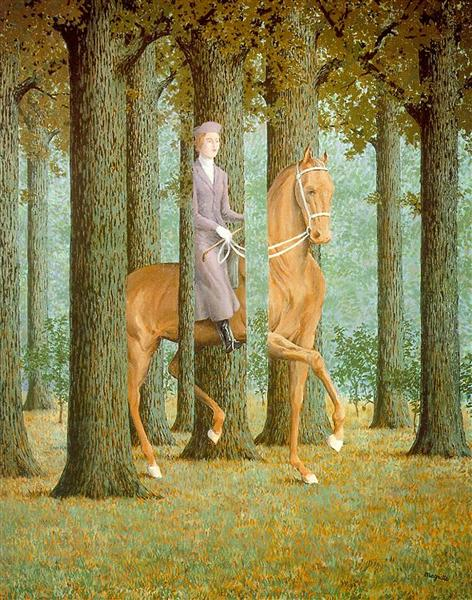
\includegraphics{img/magritte_carte_blanche.jpg}
  \caption{IO}
\end{figure}

IO ile uğraşan tipik bir fonksiyon imperatif bir programa çok benzer:

\begin{lstlisting}[language=Haskell]
  f :: IO a
  f = do
  x <- action1
  action2 x
  y <- action3
  action4 x y
\end{lstlisting}

  \begin{itemize}
    \tightlist
  \item Bir nesnenin değerini belirtmek için \lstinline!<-! kullanıyoruz.
  \item Her \st{satır} sıra kodun tipi \lstinline!IO *!, bu örnekte:
  \item \lstinline!action1 :: IO b!
  \item \lstinline!action2 x :: IO ()!
  \item \lstinline!action3 :: IO c!
  \item \lstinline!action4 x y :: IO a!
  \item \lstinline!x :: b, y :: c!
  \item Az sayıda nesnenin tipi \lstinline!IO a!'dir, bu seçmenize yardım
    eder. \st{Farklı} İnce bir ayrım olarak, burada yalın fonksiyonları doğrudan (\emph{directly})
    kullanamazsınız. Yalın fonksiyonları kullanmak için örneğin
    \lstinline!action2 (saffonksiyon x)! yazabilirsiniz.
  \end{itemize}

Bu bölümde size IO kullanmayı anlatacağım, ancak \st{nasıl} hangi yolla çalıştığını değil.
Haskell'in arı ile arı olmayan kodları \st{nasıl} hangi yolla ayırt ettiğini göreceksiniz.

Söz dizimindeki detayları anlamaya çalışmak için duraksamayın. {(\small\emph{Don’t stop because you’re trying to understand the details of the syntax}) Yanıtlar ilerleyen bölümde gelecek)}

Ne yapalım?

Kullanıcıdan bir sayı listesi girmesini isteyin. Sayıların toplamını ekrana yazdırın.

\begin{lstlisting}[language=Haskell]
  toList :: String -> [Integer]
  toList input = read ("[" ++ input ++ "]")

  main = do
  putStrLn "Bir sayi listesi girin (virgulle ayirin):"
  input <- getLine
  print $ sum (toList input)
\end{lstlisting}

Bu programın ne yaptığı oldukça açık olmalı. Tiplere biraz daha
ayrıntılı bakalım.

\begin{lstlisting}
  putStrLn :: String -> IO ()
  getLine  :: IO String
  print    :: Show a => a -> IO ()
\end{lstlisting}

Daha da ilginç biçimde , \lstinline!do! bloğunun içindeki her deyimin
\lstinline!IO a! tipinde olduğuna ilgi gösterelim.

\begin{lstlisting}[language=Haskell]
  main = do
  putStrLn "Enter ... " :: IO ()
  getLine               :: IO String
  print Something       :: IO ()
\end{lstlisting}

Ayrıca \lstinline!<-! iminin etkisine de ilgi gösterelim.

\begin{lstlisting}
  do
  x <- something -- bir nesler
\end{lstlisting}

\lstinline!something :: IO a! tipinde ise \lstinline!x :: a!'dir.

\lstinline!IO! kullanımıyla ilgili başka bir önemli \st{nokta} ayrıntı da şudur:
\lstinline!do! bloğunun içindeki tüm \st{satırlar} kod sıraları şu iki türden birindeki
olmalı:

\begin{lstlisting}[language=Haskell]
  action1             :: IO a
  -- bu durumda, a = ()
\end{lstlisting}

yada

\begin{lstlisting}[language=Haskell]
  deger <- action2    -- ki burada
  -- bar z t :: IO b
  -- deger   :: b
\end{lstlisting}

Bu iki tür komut aksiyonları sıralamanın iki değişik yolunu anlatıyor.
Bu \st{cümlenin} tümcenin anlamı önümüzdeki bölümün sonunda netleşecek.

Şimdi programımızın nasıl davrandığına bakalım. Örneğin, kullanıcı
\st{garip} sıradışı bir nes girerse ne olacak? Deneyelim:

\begin{lstlisting}
  % runghc 02_progressive_io_example.lhs
  Enter a list of numbers (separated by comma):
  foo
  Prelude.read: no parse
\end{lstlisting}

Püf! \st{Garip} Değişik bir yanıl mesajından sonra programımız çöktü! İlk
iyileştirmemiz daha anlaşılır bir yanıl mesajı vermek olsun.

Bunu yapmak için önce bir neslerin yanlış gittiğini \st{tespit edebilmemiz}
saptayabilmemiz
gerekiyor. İşte bunu yapmanın bir yolu: \lstinline!Maybe! (Türkçesi:
``belki'') tipini kullanmak. Bu Haskell'de sık kullanılan bir tiptir.

\begin{lstlisting}[language=Haskell]
  import Data.Maybe
\end{lstlisting}

Peki bu nedir ki? \lstinline!Maybe! bir tane parametre alan bir tiptir.
Tanımı da şudur:

\begin{lstlisting}[language=Haskell]
  data Maybe a = Nothing | Just a
\end{lstlisting}

Bu bir değer okumaya yada \st{yaratmaya} oluşturmaya çalışırken bir yanıl olduğunu
\st{ifade etmenin} belirtmenin güzel bir yoludur. \lstinline!maybeRead! fonksiyonu bunun iyi
bir örneği. Bu \lstinline!read!'e \footnote{Ki kendisi JavaScript'te
  JSON bulunduran bir karakter dizisi üzerinde \lstinline!eval!
  çalıştırmaya çok benzer. (Çevirmen notu: \lstinline!JSON.parse! daha
  iyi çözüm olabilir.)} benzer bir fonksiyon, ancak bir nesler yanlış
giderse dönen değer \lstinline!Nothing! olacak. Bir değer
okuyabilirse, dönen değer \lstinline!Just <değer>! olacak. Bu fonksiyonu
çok anlamaya çalışmayın; \lstinline!read!'den daha alt \st{seviye} düzey bir
fonksiyon olan \lstinline!reads!'i kullanıyorum.

\begin{lstlisting}[language=Haskell]
  maybeRead :: Read a => String -> Maybe a
  maybeRead s = case reads s of
  [(x,"")]    -> Just x
  _           -> Nothing
\end{lstlisting}

Biraz daha okunaklı olması için, şu biçimde \st{giden} ilerleyen bir fonksiyon
tanımlayalım: Karakter dizisinin formatı (\emph{biçemi}) yanlışsa,
\lstinline!Nothing! döndürülecek. \st{Aksi halde} Tersi durumda, örneğin ``1,2,3'' için
\lstinline!Just [1,2,3]! döndürülecek.

\begin{lstlisting}[language=Haskell]
  getListFromString :: String -> Maybe [Integer]
  getListFromString str = maybeRead $ "[" ++ str ++ "]"
\end{lstlisting}

Sonrasında tek yapmamız gereken dönen değeri ana fonksiyonumuzda test
etmek (\emph{denetlemek})

\begin{lstlisting}[language=Haskell]
  main :: IO ()
  main = do
  putStrLn "Bir sayi listesi girin (virgulle ayirin):"
  input <- getLine
  let maybeList = getListFromString input in
  case maybeList of
  Just l  -> print (sum l)
  Nothing -> error "Kotu format. Hoscakalin."
\end{lstlisting}

Kodun yanıl vermesi durumunda, iyi sayılabilecek bir yanıl mesajı göstermiş olalım.

\lstinline!main! fonksiyonunun \lstinline!do! bloğundaki her deyimin
tipinin \lstinline!IO a! formatında olduğuna \st{dikkat edin} gözatın. Tek
bilmediğiniz yapı \lstinline!error!. Ancak \lstinline!error msg! de
gerekli tipi alıyor. (burada \lstinline!IO ()!).

Bu programda \st{fark etmeniz} bilincine varmanız gereken nes,
tanımladığımız fonksiyonların tipleri.
Yazdığımız fonksiyonlar arasında yalnızca bir tanesinin tipinde
\lstinline!IO! var: \lstinline!main!. Bu demek oluyor ki
\lstinline!main! arı olmayan bir fonksiyon. Ancak \lstinline!main! içinde
arı bir fonksiyon olan \lstinline!getListFromString! kullanılıyor.
\st{Yani} Dolayısıyla yalnızca bakarak bile fonksiyonların arı olup olmadıklarını
anlayabilirsiniz.

Peki arılık neden önemlidir? Bir sürü avantajından üçü şunlar:

\begin{itemize}
  \tightlist
\item
  Arı kod \st{hakkında} üzerine \st{mantık} us yürütmek
  arı olmayan kod üzerine us
  yürütmekten çok daha kolaydır.
\item
  Arılık sizi yan etkilerden ötürü kolayca test edemeyeceğiniz
  \st{hatalardan} yanıllardan korur.
\item
  Arı fonksiyonları herhangi bir sırayla yada eş anlı olarak hiçbir
  risk olmadan \st{hesaplayabilirsiniz} bilgisaydırabilirsiniz.
\end{itemize}

İşte bu yüzden, olabildiğince \st{fazla} yüksek sayıda kodu arı fonksiyonlarla
yazmalısınız.

Sonraki adımımız kullanıcı geçerli bir \st{cevap} yanıt girene \st{kadar} dek
\st{tekrar tekrar} yinelecek biçimde sormak olsun.

İlk bölümü \st{aynen} olduğu gibi kullanabiliriz:

\begin{lstlisting}[language=Haskell]
  import Data.Maybe

  maybeRead :: Read a => String -> Maybe a
  maybeRead s = case reads s of
  [(x,"")]    -> Just x
  _           -> Nothing
  getListFromString :: String -> Maybe [Integer]
  getListFromString str = maybeRead $ "[" ++ str ++ "]"
\end{lstlisting}

Şimdi kullanıcı doğru bir girdi yazana dek yine soran bir fonksiyon
yazalım:

\begin{lstlisting}
  askUser :: IO [Integer]
  askUser = do
  putStrLn "Bir sayi listesi girin (virgulle ayirin):"
  input <- getLine
  let maybeList = getListFromString input in
  case maybeList of
  Just l  -> return l
  Nothing -> askUser
\end{lstlisting}

Fonksiyonumuzun tipi \lstinline!IO [Integer]!. Bu demek oluyor ki
belirli IO aksiyonları sonucu \lstinline![Integer]! tipinde bir değer
elde ediyoruz. Kimileri bunu şöyle açıklıyor:

``IO içinde [Integer] var''

Bunun arkasındaki (\emph{ardındaki} detayları anlamak istiyorsanız, sonraki bölümü
okumanız gerekecek. Ancak IO'yu yalnızca \emph{kullanmak} istiyorsanız,
\st{biraz tekrar yapın ve} konuların üzerinden gidip tipler \st{hakkında} üzerine
düşünmeniz gerektiğini \st{hatırlayın} anımsayın.

Son olarak, \lstinline!main! fonksiyonumuz çok daha kolay:

\begin{lstlisting}[language=Haskell]
  main :: IO ()
  main = do
  list <- askUser
  print $ sum list
\end{lstlisting}

IO'ya girişimizi bitirdik. Biraz hızlıydı, değil mi? Anımsamanız
gereken temel nesler şunlar:

\begin{itemize}
  \tightlist
\item
  \lstinline!do! bloğunun içinde, her deyim \lstinline!IO a! tipinde
  olmalı. Bu sizi belli deyimlere \st{kısıtlıyor} sınırlıyor. Örneğin,
  \lstinline!getLine!, \lstinline!print!, \lstinline!putStrLn!, \st{vs.} de bunun gibi.
\item
  Arı fonksiyonları olabildiğince arı olmayan bölümlerin dışında tutmaya
  çalışın, işin \st{mümkün olduğunca} olabildiğince büyük bölümünü arı fonksiyonlara
  yaptırın.
\item
  \lstinline!IO a!, \lstinline!a! tipinde bir eleman döndüren IO
  aksiyonu demektir. \lstinline!IO! aksiyonu \st{temsil eder} simgeler,
  \lstinline!IO a! esasında bir fonksiyonun tipidir. Daha \st{fazlasını
  merak ediyorsanız} ötesi ile ilgileniyorsanız sonraki bölümü okuyun.
\end{itemize}

Biraz çalışırsanız, \lstinline!IO! kullanabiliyor olmalısınız.

Alıştırma: Tüm argümanlarının toplamını alan bir program yazın. İpucu:
  \lstinline!getArgs! fonksiyonunu kullanın.

\section{IO'nun Püf Noktası}\label{ionun-puxfcf-noktasux131}

\begin{figure}[htbp]
  \centering
  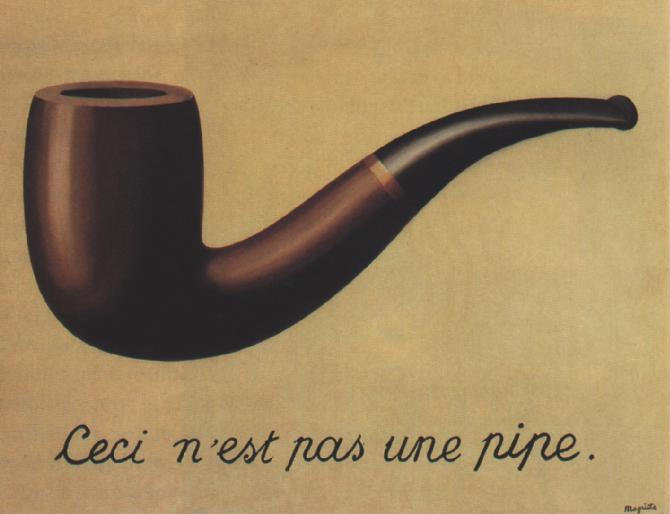
\includegraphics[width=0.5\linewidth]{img/magritte_pipe.jpg}
  \caption{Bu bir pipo degildir}
\end{figure}

Arı olan ile arı olmayan kodları ayırmak için, \lstinline!main! \st{dünyanın}
  tüm ortamın durumunu değiştiren bir fonksiyon olarak tanımlanır.

\begin{lstlisting}[language=Haskell]
  main :: World -> World
\end{lstlisting}

Bir fonksiyon, yalnızca \st{ve yalnızca} bir tek bu \st{tipe sahipse} tipi içeriyorsa yan etkide bulunur. Tipik bir \lstinline!main! fonksiyonuna bakalım:

\begin{lstlisting}[language=Haskell]
  main w0 =
  let (v1,w1) = action1 w0 in
  let (v2,w2) = action2 v1 w1 in
  let (v3,w3) = action3 v2 w2 in
  action4 v3 w3
\end{lstlisting}

  Sonraki aksiyona aktarmamız gereken bir sürü geçici elemanımız var.
  (burada \lstinline!w1!, \lstinline!w2! ile \lstinline!w3!)

  \lstinline!bind! yada \lstinline!(>>=)! fonksiyonu yaratıyoruz.
  \lstinline!bind! ile artık geçici \st{isimlere ihtiyacımız} adlara gereksinimimiz yok.

\begin{lstlisting}[language=Haskell]
  main =
  action1 >>= action2 >>= action3 >>= action4
\end{lstlisting}

Bonus: Haskell'in şöyle bir söz dizimsel (sentaks) kolaylığı var:

\begin{lstlisting}[language=Haskell]
  main = do
  v1 <- action1
  v2 <- action2 v1
  v3 <- action3 v2
  action4 v3
\end{lstlisting}


Neden böyle \st{garip} alışılmadık bir söz dizimi kullandık, \st{ve} ayrıca bu \lstinline!IO! tipi \st{tam}
net olarak nedir? Anlaşılmaz duruyor ancak, değil.

Şimdilik, programımızın arı bölümlerini bir kenara bırakıp arı olmayan
bölümler üzerine yoğunlaşalım:

\begin{lstlisting}[language=Haskell]
  askUser :: IO [Integer]
  askUser = do
  putStrLn "Bir sayi listesi girin (virgulle ayirin):"
  input <- getLine
  let maybeList = getListFromString input in
  case maybeList of
  Just l  -> return l
  Nothing -> askUser

  main :: IO ()
  main = do
  list <- askUser
  print $ sum list
\end{lstlisting}

İlk tepki: İmperatif duruyor. Haskell arı olmayan kodu imperatif
gösterecek \st{kadar} ölçüde güçlüdür. Örneğin, isterseniz Haskell'de
\lstinline!while! yapısı yaratabilirsiniz. \st{Hatta}, Üstelik ayrıca \lstinline!IO! ile
uğraşman için imperatif stil genellikle daha uygundur.

Ancak notasyonun alışılmışın dışında \st{olduğunu fark etmiş olmalısınız} olduğu gözünüze ilişmiş olmalı.
Şimdi bunun \st{sebeplerini} nedenlerini detaylıca tartışalım.

Arı olmayan bir dilde, \st{dünyanın} ortamın durumu devasa, gizli bir global
değişken olarak görülebilir. Bu gizli değişkene dildeki tüm fonksiyonlar
\st{tarafından} aracılığıyla erişilebilir. Örneğin herhangi bir fonksiyon içinde bir dosya
ile okuma/yazma işlemleri yapabilirsiniz. Dosyanın var olup olmaması
``ortam''ınızın alabileceği olası durumlardır.

Haskell'de bu durum gizli değildir. \st{Tam} Direkt tersine, Haskell'de
\lstinline!main!'in ortamınızın durumunu değiştirme olasılığı olduğu
ayrıca özel olarak belirtilir. Bu fonksiyonun tipi şunun gibi bir nesdir:

\begin{lstlisting}[language=Haskell]
  main :: World -> World
\end{lstlisting}

Bu değişkene tüm fonksiyonların erişimi yoktur. Erişimi olan
fonksiyonlar arı değildir. (Global) ortam değişkenine erişimi olmayan
fonksiyonlar ise arıdır. \footnote{Bu kurala uymayan kimi güvenli olmayan
  \st{istisnalar} dış durumlar da var. Ancak belki yanıl ayıklama amacı dışında hiçbir gerçek
  uygulamada böyle bir kullanım görmezsiniz.}

Haskell, ortamın durumunu \lstinline!main! fonksiyonuna bir girdi
değişkeni olarak görür. Ancak \lstinline!main!'in esas tipi şuna daha
yakındır: \footnote{\st{Merak edenler} İlgilenenler için: gerçek tip şöyle:\\
  \lstinline!data IO a = IO {unIO :: State# RealWorld -> (# State# RealWorld, a #)}!.
  \lstinline!#! imi optimizasyonla ilgili\st{, ve} olup ben örneğimde alan
  yerlerini değiştirdim. Ancak ana \st{fikir} düşünce bu.}

\begin{lstlisting}[language=Haskell]
  main :: World -> ((),World)
\end{lstlisting}

\lstinline!()! tipi birim tipidir. Burda görülecek bir nes yok.

Şimdi bunu \st{aklımızda} belleğimizde tutarak \lstinline!main! fonksiyonumuzu baştan
yazalım:

\begin{lstlisting}[language=Haskell]
  main w0 =
  let (list,w1) = askUser w0 in
  let (x,w2) = print (sum list,w1) in
  x
\end{lstlisting}

İlk olarak, yan etkisi olan tüm fonksiyonların şu tipte olması
gerektiğini \st{hatırlayalım} anımsayalım:

\begin{lstlisting}[language=Haskell]
  World -> (a,World)
\end{lstlisting}

Burada \lstinline!a! sonucun tipi oluyor. Örneğin \lstinline!getChar!
fonksiyonu bu durumda \lstinline!World -> (Char,World)! tipindedir.

Özen gösterilmesi gereken \st{diğer bir şey} öteki ayrıntı ise
\st{hesaplama} kalkülasyon / değerlendirme sırası.
Örneğin \lstinline!f a b!'yi \st{hesaplarken} kalküle ederken birden \st{fazla} çok
seçeneğiniz var:

\begin{itemize}
  \tightlist
\item
  önce \lstinline!a!'yi, sonra \lstinline!b!'yi, sonra da
  \lstinline!f a b!'yi kalküle et.
\item
  önce \lstinline!b!'yi, sonra \lstinline!a!'yi, sonra da
  \lstinline!f a b!'yi kalküle et.
\item
  \lstinline!a!'yi ve \lstinline!b!'yi paralel olarak, sonra da
  \lstinline!f a b!'yi kalküle et.
\end{itemize}

Bu böyle çünkü dilin arı \st{kısmında} yanında çalışıyoruz.

Şimdi, \lstinline!main! fonksiyonuna bakarsanız, ilk \st{satırı} kod sırası ikinci
kod sırasından önce kalküle etmemiz gerektiği açık, çünkü ikinci kod sırasında birincidekinden
elde ettiğiniz bir değeri parametre olarak kullanıyorsunuz.

Bu işe yarıyor. Derleyici her adımda yeni bir gerçek global ortam tanımı / kodu
(\emph{id}) sağlıyor. Gizli olarak, \lstinline!print! şöyle işliyor:

\begin{itemize}
  \tightlist
\item
  ekrana bir nes yazdır
\item
  global ortamın id'sini değiştir.
\item
  \lstinline!((), yeni global ortam id'si)! değerini döndür.
\end{itemize}

Şimdi, \lstinline!main! fonksiyonunun stiline bakarsanız, biraz
değişik olduğunu göreceksiniz. \st{Aynısıni} Tıpatıp özdeşini \lstinline!askUser! fonksiyonuna
da uygulayalım:

\begin{lstlisting}[language=Haskell]
  askUser :: World -> ([Integer],World)
\end{lstlisting}

Öncesi:

\begin{lstlisting}[language=Haskell]
  askUser :: IO [Integer]
  askUser = do
  putStrLn "Bir sayi listesi girin:"
  input <- getLine
  let maybeList = getListFromString input in
  case maybeList of
  Just l  -> return l
  Nothing -> askUser
\end{lstlisting}

Sonrası:

\begin{lstlisting}[language=Haskell]
  askUser w0 =
  let (_,w1)     = putStrLn "Bir sayi listesi girin:" in
  let (input,w2) = getLine w1 in
  let (l,w3)     = case getListFromString input of
  Just l   -> (l,w2)
  Nothing  -> askUser w2
  in
  (l,w3)
\end{lstlisting}

Benzer, ancak biraz daha değişik. Tüm şu geçici \lstinline!w!'lere bakın.

Çıkarılacak \st{ders} öğreti şu: Arı fonksiyonel dillerdeki naif IO uygulamaları
\st{gariptir!} sıradışıdır!

Şanslıyız ki, bu sorunu \st{halletmek} çözümlemek için daha iyi bir yol var. Bir \st{kalıp} desen
görüyoruz, her kod sırası şu biçimde:

\begin{lstlisting}[language=Haskell]
  let (y,w') = action x w in
\end{lstlisting}

Herhangi bir kod sırası için ilk \lstinline!x! argümanı gerekmese bile. Dönen
sonucun tipi bir ikili, \mbox{\lstinline!(sonuç, yeniGlobalOrtamDegeri)!} Her
\lstinline!f! fonksiyonu şuna benzer bir \st{tipe sahip olmak} tipi içermek zorunda:

\begin{lstlisting}[language=Haskell]
  f :: World -> (a,World)
\end{lstlisting}

Her \st{zaman} durumda \st{ayni} özdeş \st{kalıbı} deseni \st{takip ettiğimize} izlediğimize
\st{dikkat edin} özel ilgi gösterin:

\begin{lstlisting}[language=Haskell]
  let (y,w1) = action1 w0 in
  let (z,w2) = action2 w1 in
  let (t,w3) = action3 w2 in
  ...
\end{lstlisting}

Her aksiyon hiçten(0) n'ye \st{kadar} dek parametre alabilir. \st{Ve} Ayrıca özellikle, her
aksiyon bir üstündeki kod sırasının sonucundan parametre alabilir.

Örneğin, şöyle diyebiliriz:

\begin{lstlisting}[language=Haskell]
  let (_,w1) = action1 x w0   in
  let (z,w2) = action2 w1     in
  let (_,w3) = action3 x z w2 in
  ...
\end{lstlisting}

\st{Ve tabii ki} Buradan doğal olarak \lstinline!actionN w :: (World) -> (a,World)!.

Önemli: \st{Dikkat edilmesi} Göz atılması gereken iki desen var:

\begin{lstlisting}[language=Haskell]
  let (x,w1) = action1 w0 in
  let (y,w2) = action2 x w1 in
\end{lstlisting}

  ile

\begin{lstlisting}[language=Haskell]
  let (_,w1) = action1 w0 in
  let (y,w2) = action2 w1 in
\end{lstlisting}

\begin{figure}[htbp]
  \centering
  
\includegraphics{img/jocker_pencil_trick.jpg}
  \caption{Joker}
\end{figure}

Şimdi biraz \st{sihirbazlık} oyunculuk yapalım. Geçici global ortam sembolünü ``yok edelim''.
İki kod sırasını \lstinline!bind! ile birbirine bağlayacağız. İşe
\lstinline!bind! fonksiyonunu tanımlayarak başlayalım. Fonksiyonun tipi
başta biraz korkutucu gelebilir:

\begin{lstlisting}[language=Haskell]
  bind :: (World -> (a,World))
  -> (a -> (World -> (b,World)))
  -> (World -> (b,World))
\end{lstlisting}

Ancak anımsayın ki \lstinline!(World -> (a,World))! IO aksiyonlarının
tipidir. Daha açık olması için ona yeni bir ad verelim:

\begin{lstlisting}[language=Haskell]
  type IO a = World -> (a, World)
\end{lstlisting}

Kimi fonksiyon örnekleri:

\begin{lstlisting}[language=Haskell]
  getLine :: IO String
  print :: Show a => a -> IO ()
\end{lstlisting}

\lstinline!getLine! global ortamı parametre olarak alıp 
\lstinline!(String,World)! ikilisini döndüren bir IO aksiyonudur.
Bu şöyle özetlenebilir: \lstinline!getLine!, \lstinline!IO String!
tipindedır ki bunu ``IO içine gömülmüş'' String döndüren bir IO
aksiyonu olarak görebiliriz.

\lstinline!print! fonksiyonu da ayrıca ilginçtir. Gösterilebilir bir
argüman alır, ancak esasında iki argüman almaktadır. İlki ekrana
yazdırılacak değerdir, ikincisi de global ortamın durumudur. Sonrasında ise
\lstinline!((),World)! ikilisini döndürür. Bu fonksiyonun global ortamın
durumunu değiştirdiği ancak başka bir veri üretmediği anlamına gelir.

Bu tip, \lstinline!bind! fonksiyonun tipini \st{basitleştirmemize} yalınlaştırmamıza  yardımcı
olur:

\begin{lstlisting}[language=Haskell]
  bind :: IO a
  -> (a -> IO b)
  -> IO b
\end{lstlisting}

Bu demek oluyor ki \lstinline!bind! fonksiyonu iki IO aksiyonunu
parametre olarak \st{alıyor ve} alıp başka bir IO aksiyonunu geri döndürüyor.

Önemli desenleri \st{tekrar} yeniden anımsayın. İlki şuydu:

\begin{lstlisting}[language=Haskell]
  let (x,w1) = action1 w0 in
  let (y,w2) = action2 x w1 in
  (y,w2)
\end{lstlisting}

Fonksiyonların tiplerine bakalım:

\begin{lstlisting}[language=Haskell]
  action1  :: IO a
  action2  :: a -> IO b
  (y,w2)   :: IO b
\end{lstlisting}

Tanıdık gelmiyor mu?

\begin{lstlisting}[language=Haskell]
  (bind action1 action2) w0 =
  let (x, w1) = action1 w0
  (y, w2) = action2 x w1
  in  (y, w2)
\end{lstlisting}

Amacımız World argümanını bu fonksiyonla gizlemek. Örnek olarak, şunu
gerçekleştirmek istediğimizi varsayalım:

\begin{lstlisting}[language=Haskell]
  let (line1,w1) = getLine w0 in
  let ((),w2) = print line1 in
  ((),w2)
\end{lstlisting}

Şimdi, \lstinline!bind! fonksiyonunu kullanarak:

\begin{lstlisting}[language=Haskell]
  (res,w2) = (bind getLine (\l -> print l)) w0
\end{lstlisting}

\lstinline!print! fonksiyonu \lstinline!(World -> ((),World))! tipinde
olduğu için, \lstinline!res = ()! (boş tip) Bundaki \st{sihirbazliği}
oyunu görmediyseniz, bu \st{sefer} kez üç \st{satırla} sıra kodla deneyelim:

\begin{lstlisting}[language=Haskell]
  let (line1,w1) = getLine w0 in
  let (line2,w2) = getLine w1 in
  let ((),w3) = print (line1 ++ line2) in
  ((),w3)
\end{lstlisting}

Bu da şuna denk:

\begin{lstlisting}[language=Haskell]
  (res,w3) = (bind getLine (\line1 ->
  (bind getLine (\line2 ->
  print (line1 ++ line2))))) w0
\end{lstlisting}

Bir \st{şeyi fark ettiniz mi?} nes ilginizi çekti mi? Evet, artık hiçbir yerde geçici World
değişkenleri kullanılmıyor. \st{Sihirbazlik} Büyücülük gibi.

Daha iyi bir notasyon kullanabiliriz. \lstinline!bind! yerine
\lstinline!(>>=)! kullanalım. \lstinline!(>>=)!, \lstinline!(+)! gibi
bir iç notasyonlu fonksiyondur; ki şöyle çalışır:
\lstinline!3 + 4 ⇔ (+) 3 4!

Ho Ho Ho! Herkese Mutlu Noeller! Haskell bize söz dizimsel kolaylık
sağlıyor:

\begin{lstlisting}[language=Haskell]
  do
  x <- action1
  y <- action2
  z <- action3
  ...
\end{lstlisting}

yerine şöyle yazabiliriz:

\begin{lstlisting}[language=Haskell]
  action1 >>= (\x ->
  action2 >>= (\y ->
  action3 >>= (\z ->
  ...
\end{lstlisting}

\lstinline!action2! içinde \lstinline!x!, \lstinline!action3! içinde hem
\lstinline!x! hem de \lstinline!y! değişkenlerini kullanabildiğinize
dikkat edin.

Peki \lstinline!<-! kullanmayan kodlarda ne yapacağız? Kolay,
\lstinline!blindBind! diye başka bir fonksiyon tanımlayalım:

\begin{lstlisting}[language=Haskell]
  blindBind :: IO a -> IO b -> IO b
  blindBind action1 action2 w0 =
  bind action (\_ -> action2) w0
\end{lstlisting}

Bu tanımı daha açık olması için yalınlaştırmadım. Doğal olarak daha yalın bir
notasyon kullanabiliriz, bunun için \lstinline!(>>)! operatörü var.

\begin{lstlisting}[language=Haskell]
  do
  action1
  action2
  action3
\end{lstlisting}

Şuna dönüşüyor:

\begin{lstlisting}[language=Haskell]
  action1 >>
  action2 >>
  action3
\end{lstlisting}

Kullanışlı bir fonksiyon daha var.

\begin{lstlisting}[language=Haskell]
  putInIO :: a -> IO a
  putInIO x = IO (\w -> (x,w))
\end{lstlisting}

Bu arı değerleri IO bağlamına sokmak için kullanılan genel bir yoldur.
\lstinline!putInIO! için kullanılan genel ad \lstinline!return!'dür.
Haskell öğrenirken bu oldukça kötü bir adlandırmadır çünkü Haskell'deki
\lstinline!return! alışık olduğunuzden çok \st{farklıdır} değişiktir.

Örneğimizi çevirerek bu bölümü bitirelim:

\begin{lstlisting}[language=Haskell]
  askUser :: IO [Integer]
  askUser = do
  putStrLn "Bir sayi listesi girin (virgullerle ayirin):"
  input <- getLine
  let maybeList = getListFromString input in
  case maybeList of
  Just l  -> return l
  Nothing -> askUser

  main :: IO ()
  main = do
  list <- askUser
  print \$ sum list
\end{lstlisting}

Şu \st{hale} duruma geliyor:

\begin{lstlisting}[language=Haskell]
  import Data.Maybe

  maybeRead :: Read a => String -> Maybe a
  maybeRead s = case reads s of
  [(x,"")]    -> Just x
  _           -> Nothing
  getListFromString :: String -> Maybe [Integer]
  getListFromString str = maybeRead $ "[" ++ str ++ "]"
  askUser :: IO [Integer]
  askUser =
  putStrLn "Bir sayi listesi girin (virgullerle ayirin):" >>
  getLine >>= \input ->
  let maybeList = getListFromString input in
  case maybeList of
  Just l -> return l
  Nothing -> askUser

  main :: IO ()
  main = askUser >>=
  \list -> print $ sum list
\end{lstlisting}

Çalıştığını doğrulamak için derleyebilirsiniz.

\lstinline!(>>)! ile \lstinline!(>>=)! olmadan ne yolla olacağını düşünün.

\section{Monad}\label{monad}

\begin{figure}[htbp]
  \centering
  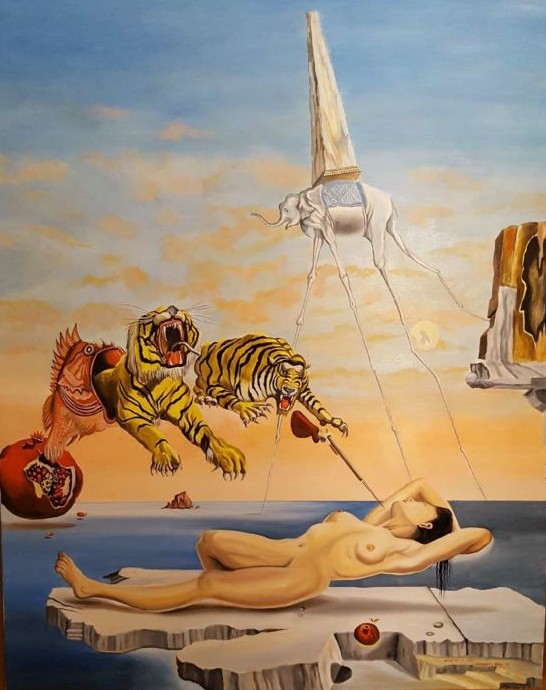
\includegraphics{img/dali-reve.jpg}
  \caption{Monad}
\end{figure}

Artık bu \st{sırrı} gizemi açıklayabiliriz: \lstinline!IO! bir \emph{monad}dir.
Monad olmak, \lstinline!do! notasyonu ile belirli söz dizimsel
kolaylıklara \st{sahip} iye olmak demektir. Ancak temel olarak, kodunuzun akışını
kolaylaştıracak belirli kod desenlerine erişim sağlar.

  Önemli ayrıntılar:
  \begin{itemize}
  \item Monadlar etkilerle ilgili olmak zorunda değildir! Arı  monadlar da vardır.
  \item Monadlar daha çok sıralama ile ilgilidir.
  \end{itemize}
  
Haskell'de \lstinline!Monad! bir tip klasıdır. Bu klasın bir üyesi
olmak için \lstinline!(>>=)! ile \lstinline!return! fonksiyonlarını
sağlamalısınız. \lstinline!(>>)! fonksiyonu \lstinline!(>>=)!
fonksiyonundan türer. \st{Basit} Temel olarak \lstinline!Monad! tip klası şöyle
belirtilir:

\begin{lstlisting}[language=Haskell]
  class Monad m  where
  (>>=) :: m a -> (a -> m b) -> m b
  return :: a -> m a

  (>>) :: m a -> m b -> m b
  f >> g = f >>= \_ -> g

  -- Yalnızca gecmisteki (tarihsel) nedenlerden dolayi oldugunu dusundugum
  -- bu fonksiyonu degerlendirmeye (dikkate) almayabilirsiniz
  fail :: String -> m a
  fail = error
\end{lstlisting}
\pagebreak
  Notlar:
  \begin{itemize}
  \item \lstinline!class! anahtar sözcüğü dostunuz değildir.
  Haskell'deki class nesne yönelimli programlamada karşılaştığınız class
  gibi değildir. Haskell'deki class Java'daki interface'le benzeşir.
  \lstinline!typeclass! daha iyi bir adlandırma olurdu, çünkü o tip
  grubu anlamına geliyor. Bir tipin bir klasa \st{ait} bağlı olması için, bir
  klasın tüm fonksiyonlarının o tip için sağlanabilir olması gerekiyor.

  \item Tip sınıflarının bu örneğinde, \lstinline!m! tipinin argüman alan bir
  tip olması gerekiyor, örneğin \lstinline!IO a!, ancak eş anlı olarak
  \lstinline!Maybe a!, \lstinline![a]!, de bunun gibi.

  \item Fonksiyonunuzun kullanışlı
  bir monad olması için bazı kurallara uyması gerekiyor. Eğer yapınız bu
  kurallara uymuyorsa garip şeyler gerçekleşebilir:
  \lstinline!~ return a >>= k == k a m >>= return == m m >>= (-> k x >>= h) == (m >>= k) >>= h ~!
  \end{itemize}

\subsubsection{Maybe Monad'ı}\label{maybe-monadux131}

\lstinline!Monad! tip klasının üyesi olan bir sürü değişik tip vardır.
\st{Tarif etmesi} Tanımlaması en kolay olanlarından biri de \lstinline!Maybe!'dir. 
\lstinline!Maybe! değerlerinden oluşan bir diziniz varsa, etkilemek için
monadları kullanabilirsiniz. Uzayıp giden \lstinline!if then else  !
yapılarından kurtulmak için oldukça kullanışlı bir yoldur.

Karmaşık bir banka işlemi düşünün. \st{Bakiyeniz} Kontoda kalan paranız \st{sıfırın} hiçin altına
düşmeden belli işlemleri yapabilecek \st{kadar} yeterlikte paranız varsa, 700\euro{}
kazanma \st{hakkınız} olanağınız/payınız olsun.

\begin{lstlisting}[language=Haskell]
  deposit  value account = account + value --para yatirma
  withdraw value account = account - value --para cekme

  --para kazanmaya pay kazanip kazanmadiginizi donduren fonksiyon
  eligible :: (Num a,Ord a) => a -> Bool
  eligible account =
  let account1 = deposit 100 account in
  if (account1 < 0)
  then False
  else
  let account2 = withdraw 200 account1 in
  if (account2 < 0)
  then False
  else
  let account3 = deposit 100 account2 in
  if (account3 < 0)
  then False
  else
  let account4 = withdraw 300 account3 in
  if (account4 < 0)
  then False
  else
  let account5 = deposit 1000 account4 in
  if (account5 < 0)
  then False
  else
  True

  main = do
  print $ eligible 300 -- True
  print $ eligible 299 -- False
\end{lstlisting}

Şimdi \lstinline!Maybe! kullanıp monadlardan yararlanarak
iyileştirelim:

\begin{lstlisting}[language=Haskell]
  deposit :: (Num a) => a -> a -> Maybe a
  deposit value account = Just (account + value)

  withdraw :: (Num a,Ord a) => a -> a -> Maybe a
  withdraw value account = if (account < value)
  then Nothing
  else Just (account - value)

  eligible :: (Num a, Ord a) => a -> Maybe Bool
  eligible account = do
  account1 <- deposit 100 account
  account2 <- withdraw 200 account1
  account3 <- deposit 100 account2
  account4 <- withdraw 300 account3
  account5 <- deposit 1000 account4
  Just True

  main = do
  print $ eligible 300 -- Just True
  print $ eligible 299 -- Nothing
\end{lstlisting}

Kötü değil, ancak daha da iyileştirebiliriz:

\begin{lstlisting}[language=Haskell]
  deposit :: (Num a) => a -> a -> Maybe a
  deposit value account = Just (account + value)

  withdraw :: (Num a,Ord a) => a -> a -> Maybe a
  withdraw value account = if (account < value)
  then Nothing
  else Just (account - value)

  eligible :: (Num a, Ord a) => a -> Maybe Bool
  eligible account =
  deposit 100 account >>=
  withdraw 200 >>=
  deposit 100  >>=
  withdraw 300 >>=
  deposit 1000 >>
  return True

  main = do
  print $ eligible 300 -- Just True
  print $ eligible 299 -- Nothing
\end{lstlisting}

Monadların kodumuzu daha \st{zarifleştirmenin} şirinleştirmenin iyi bir yolu olduğunu gösterdik. Özellikle bakın ki, bu tip bir kod düzenlemesi, özellikle
\lstinline!Maybe!, pek çok imperatif dilde de uygulanabilir. Esasında, bu tip
bir yapıyı normalde de yapıyoruz.

  Önemli bir ayrıntı: Dizideki ilk elemanın \lstinline!Nothing! olarak
  kalküle edilmesi tüm işlemi durduracaktır. Bu demek oluyor ki, tüm
  kod sıralarını işletmiyorsunuz. Üşengeçlik sayesinde bunun için \st{fazladan} ekstradan bir nes yapmanıza gerek yok.

Bunu göz önünde bulundurarak \lstinline!Maybe! için \lstinline!(>>=)!
fonksiyonunu şöyle tanımlayabilirsiniz:

\begin{lstlisting}[language=Haskell]
  instance Monad Maybe where
  (>>=) :: Maybe a -> (a -> Maybe b) -> Maybe b
  Nothing  >>= _  = Nothing
  (Just x) >>= f  = f x

  return x = Just x
\end{lstlisting}

Bu \st{basit} temel örnek ile \lstinline!Maybe! monadının ne denli kullanışlı
olabileceğini \st{ve nasıl} de ne yolla kullanılabileceğini gördük. Ancak daha iyi bir örnek için listelere bakalım.
\pagebreak

\subsubsection{Liste Monad'ı}\label{liste-monadux131}
\begin{figure}% [htbp]
  \centering
  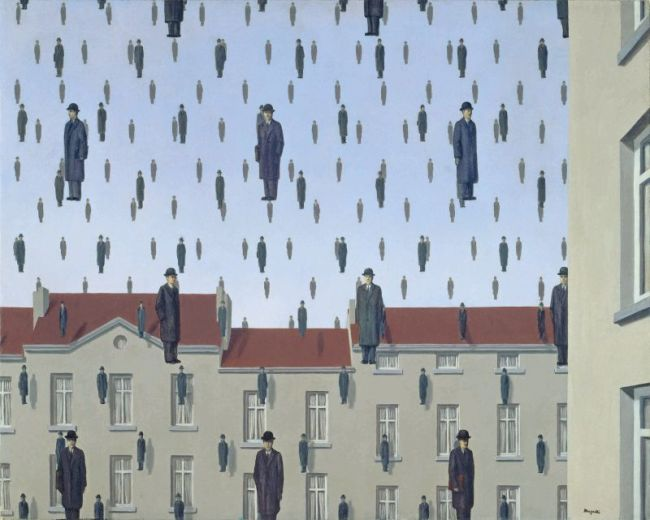
\includegraphics{img/golconda.jpg} % [width=0.8\linewidth]
  \caption{Golconda (Listeler)}
\end{figure}

Liste monadı deterministik (belirlenimci) olmayan \st{hesaplamaları} kalkülasyonları simüle etmemize yardımcı olur. Şöyle:

\begin{lstlisting}[language=Haskell]
  import Control.Monad (guard)

  allCases = [1..10]

  resolve :: [(Int,Int,Int)]
  resolve = do
  x <- allCases
  y <- allCases
  z <- allCases
  guard $ 4*x + 2*y < z
  return (x,y,z)

  main = do
  print resolve
\end{lstlisting}

\st{Resmen sihirbazlık} Açıkça oyunbazlık.

\begin{lstlisting}[language=Haskell]
  [(1,1,7),(1,1,8),(1,1,9),(1,1,10),(1,2,9),(1,2,10)]
\end{lstlisting}

Liste monadı için, şöyle bir söz dizimsel kolaylık da vardır:

\begin{lstlisting}[language=Haskell]
  print $ [ (x,y,z) | x <- allCases,
    y <- allCases,
    z <- allCases,
    4*x + 2*y < z ]
\end{lstlisting}

Tüm monadları sıralamayacağım, ancak bir sürü monad bulunmakta. Arı
dillerdeki belli kavramlar monad kullanımı ile yalınlaştırılmıştır.
Monadlar özellikle şunlar için kullanışlıdır:

\begin{itemize}\tightlist
\item IO
\item deterministik olmayan kalkülasyonlar
\item (sözde) gelişigüzel sayı üretimi
\item konfigürasyon durumunu tutma
\item yazma durumu
\end{itemize}

Buraya dek beni izleyebildiyseniz, başardınız demektir!
Monadları öğrendiniz. \footnote{Doğal olarak \st{alışana ve tamamen} alışıp tümüyle anlayana dek
  çalışmanız gerekiyor. Ancak bu yönde büyük bir adım attınız bile.}

\part{Ekler}\label{ekler}

Bu bölüm doğrudan Haskell'le ilgili değil. Kimi ayrıntılı açıklamalar
için okuyabilirsiniz.

\section{Sonsuz Ağaçlara İlişkin}\label{sonsuz-aux11fauxe7lar-hakkux131nda}

\hyperref[33-sonsuz-yapux131lar]{Sonsuz Yapılar} bölümünde kimi yalın
yapılar görmüştük. Ancak ağacımızdan iki özellik çıkartmıştık:

\begin{enumerate}
\def\labelenumi{\arabic{enumi}.}\tightlist
\item yinelenen (duplike) düğümlerin (node) olmaması
\item düzgün sıralı ağaç olması
\end{enumerate}

Bu bölümde ilk özelliği sağlamaya (iletmeye) çalışacağız. İkincisiyle ilgili olarak
şimdilik pek bir nes yapmayacağız ancak onu ne yaparak olabildiğince düzgün sıralı
tutabileceğimizi tartışacağız.

{\emph\small(In this section we will try to keep the first property. Concerning
  the second one, we must relax it but we’ll discuss how to keep it as much as possible.)}

İlk adımımız (sözde) gelişigüzel bir sayı listesi oluşturmak olsun:

\begin{lstlisting}[language=Haskell]
  shuffle = map (\x -> (x*3123) `mod` 4331) [1..]
\end{lstlisting}

\lstinline!treeFromList! fonksiyonunun tanımını anımsayalım

\begin{lstlisting}[language=Haskell]
  treeFromList :: (Ord a) => [a] -> BinTree a
  treeFromList []    = Empty
  treeFromList (x:xs) = Node x (treeFromList (filter (<x) xs))
  (treeFromList (filter (>x) xs))
\end{lstlisting}

\lstinline!treeTakeDepth! de şöyleydi:

\begin{lstlisting}[language=Haskell]
  treeTakeDepth _ Empty = Empty
  treeTakeDepth 0 _     = Empty
  treeTakeDepth n (Node x left right) = let
  nl = treeTakeDepth (n-1) left
  nr = treeTakeDepth (n-1) right
  in
  Node x nl nr
\end{lstlisting}

Programımız da şu biçimde:

\begin{lstlisting}[language=Haskell]
  main = do
  putStrLn "take 10 shuffle"
  print $ take 10 shuffle
  putStrLn "\ntreeTakeDepth 4 (treeFromList shuffle)"
  print $ treeTakeDepth 4 (treeFromList shuffle)
\end{lstlisting}

\begin{lstlisting}
  % runghc 02_Hard_Part/41_Infinites_Structures.lhs
  take 10 shuffle
  [3123,1915,707,3830,2622,1414,206,3329,2121,913]
  treeTakeDepth 4 (treeFromList shuffle)

  < 3123
  : |--1915
  : |  |--707
  : |  |  |--206
  : |  |  `--1414
  : |  `--2622
  : |     |--2121
  : |     `--2828
  : `--3830
  :    |--3329
  :    |  |--3240
  :    |  `--3535
  :    `--4036
  :       |--3947
  :       `--4242
\end{lstlisting}

Hey, sonlanıyor! Ancak bir göz atın, program yalnızca dallara koyulabilecek veri
olduğu sürece çalışacak.

Örneğin:

\begin{lstlisting}[language=Haskell]
  treeTakeDepth 4 (treeFromList [1..])
\end{lstlisting}

sonsuza dek çalışacak çünkü \lstinline!filter (<1) [2..]! deyiminin
ilk elemanını almaya çabalayacak. Ancak \lstinline!filter! fonksiyonu
sonucun boş liste olduğunu anlayacak ölçüde soybağ değil.

Bunlar da okur için alıştırma olarak kalsın:

\begin{itemize}
  \tightlist
\item
  \lstinline!treeTakeDepth n (treeFromList shuffle)! deyimini sonsuz
  döngüye sokacak bir \lstinline!n! değeri olduğunu kanıtlayın.
\item
  \lstinline!n! için bir üst sınır bulun.
\item
  Hiçbir \lstinline!shuffle! listesinin programı bitiremeyeceğini
  kanıtlayın.
\end{itemize}

Bu sorunları çözmek için \lstinline!treeFromList! ve \lstinline!shuffle!
fonksiyonlarımızı biraz değiştireceğiz.

İlk sorunumuz, \lstinline!shuffle! fonksiyon tanımımızda sonsuz ayrık
sayı üreten bir yapı olmaması. Yalnızca \lstinline!4331! ayrık sayı
ürettik. Bunu çözmek için daha iyi bir \lstinline!shuffle! fonksiyonu
yazalım.

\begin{lstlisting}[language=Haskell]
  shuffle = map rand [1..]
  where
  rand x = ((p x) `mod` (x+c)) - ((x+c) `div` 2)
  p x = m*x^2 + n*x + o -- bir polinom
  m = 3123
  n = 31
  o = 7641
  c = 1237
\end{lstlisting}

Bu \lstinline!shuffle! fonksiyonunun (umarız ki) bir alt yada üst limiti
yok. Ancak daha iyi bir gelişigüzel sayı fonksiyonu sonsuz döngüye girmeyi
engellemiyor.

Genel olarak, \lstinline!filter (<x) xs!'in boş liste olup olmadığını
anlamıyoruz. Öyleyse bu sorunu çözmek için, ikili ağacımızı oluştururken
yanıl verdirmeyi deneyelim. Kodumuzun bu yeni versiyonu düğümleri için şu
özelliği olan bir ikili ağaç oluşturacak:

Sol alt ağaçtaki herhangi bir eleman, kökün değeriden daha küçük olmalı.

Özellikle göz atın ki genel olarak sıralı bir ikili ağaç olarak kalacak.
Ayrıca, yapı \st{itibarıyla} olarak, her düğüm değeri ağaçta tek olacak,
\st{tekrarlanmayacak} yinelenmeyecek.

\begin{lstlisting}[language=Haskell]
  treeFromList :: (Ord a, Show a) => [a] -> BinTree a
  treeFromList []    = Empty
  treeFromList (x:xs) = Node x left right
  where
  left = treeFromList $ safefilter (<x) xs
  right = treeFromList $ safefilter (>x) xs
\end{lstlisting}

Bu yeni \lstinline!safefilter! fonksiyonu \lstinline!filter!
fonksiyonuna neredeyse denk ancak liste sonsuzsa, sonsuz döngüye
girmiyor. Ardarda 10000 değerin testi olumsuz çıkarsa, bunu
aramanın sonu olarak değerlendiriyor.

\begin{lstlisting}[language=Haskell]
  safefilter :: (a -> Bool) -> [a] -> [a]
  safefilter f l = safefilter' f l nbTry
  where
  nbTry = 10000
  safefilter' _ _ 0 = []
  safefilter' _ [] _ = []
  safefilter' f (x:xs) n =
  if f x
  then x : safefilter' f xs nbTry
  else safefilter' f xs (n-1)
\end{lstlisting}

Şimdi programı çalıştırıp mutlu olabilirsiniz:

\begin{lstlisting}[language=Haskell]
  main = do
  putStrLn "take 10 shuffle"
  print $ take 10 shuffle
  putStrLn "\ntreeTakeDepth 8 (treeFromList shuffle)"
  print $ treeTakeDepth 8 (treeFromList $ shuffle)
\end{lstlisting}

Ekrana yazdırılan her değerin yazma anının \st{farklı} değişik olduğunu \st{fark
etmelisiniz} sezinlemelisiniz. Bunun nedeni Haskell'in her değeri yalnızca gereksinimi olduğu
anda kalküle etmesi. \st{Ve} Ek olarak bu durumda, bu an ekrana \st{ yazdırılacağı zaman} yazdırılacağında.

Daha da etkileyici bir nes görmek için \lstinline!depth! değerini
\lstinline!8!'den \lstinline!100!'e çıkarın. RAM'inizi boğmadan
çalışacak! Akış \st{ve hafıza} ile bellek yönetimi Haskell \st{tarafından} aracılığı ile doğal olarak
yapılıyor.

Bu da okura alıştırma olarak kalsın:

\begin{itemize} \tightlist
\item  \lstinline!deep! ve \lstinline!nbTry! için yüksek değişmez (sabit) değer ile
  bile, iyi biçimde çalışıyor gibi gözüküyor. Ancak en kötü durumda üstel
  olabilir. \lstinline!treeFromList! için olabilecek kötü bir liste
  oluşturun. \emph{ipucu}:
  {[}0,-1,-1,\ldots{}.,-1,1,-1,\ldots{},-1,1,\ldots{}{]} listesini
  düşünün.
\item  \lstinline!safefilter! fonksiyonunu şöyle tanımlamayı denedim:

  \begin{lstlisting}[language=Haskell]
  safefilter' f l = if filter f (take 10000 l) == []
  then []
  else filter f l
\end{lstlisting}
\end{itemize}

* Neden çalışmayıp sonsuz döngüye girebileceğini açıklayın.
* \lstinline!shuffle!`in artan sınırlarla gerçek bir gelişigüzel liste
olduğunu \st{farz edin} varsayın. Bu yapı üzerinde biraz çalışırsanız, bu yapının bir
olasılıkla sonlu olduğunu \st{fark edeceksiniz} yakalayacaksınız.
Aşağıdaki kodu kullanarak (hiç \lstinline!safefilter! yokmuş gibi doğrudan \lstinline!safefilter'!
kullanın) \lstinline!f! için bir olasılıkla treeFromList' shuffle'ın sonlu
olduğu bir tanım bulup kanıtlayın. Önemli: Bu yalnızca bir konjektür.

\section{Mutsözleri}\label{teux15mutsozleri}

{\color{blue} r/haskell}\footnote{reddit.com/r/haskell} ile
{\color{blue} r/programming}\footnote{reddit.com/r/programming}
esenlikler diliyorum. Yorumları bana çok yardımcı oldu.

Özellikle, Emm\footnote{github\centerdot com/Emm, Danimarkab, www.impero\centerdot com}'e, İngilizcemi
düzeltmekle uğraştığı süre için binlerce kez mutsözlerimi iletirim.

  Çevirmen Notu (Joomy Korkut): Klavyemde Türkçe karakterler olmadığı için zoraken
  deasciifier\footnote{github\centerdot com/joom/turkish-deasciifier.vim}
  kullanıyorum. Yazıda herhangi bir Türkçe karakter yada çeviri yanlışı
  bulursanız, beni bilgilendirirseniz, yada \emph{pull request} yollayarak
  düzeltirseniz çok sevinirim. Bu, daha iyi çevirilebileceğini düşündüğünüz
  bölümler için de geçerli. Esenlikler.

\paragraph{Dipnotlar}\label{dipnotlar}

No.1

\newpage

\part{Özgür Belge Lisansı}

% \titleformat{\section}[runin]{\normalfont\scshape}{}{0pt}{}\titlespacing{\section}{\parindent}{*2}{\wordsep}

{\Large GNU Free Documentation License\itshape Version 1.2, Nov 2002}\label{gfdl}
\footnote{tr\centerdot pardus-wiki\centerdot org, orjinal kaynak: gnu\centerdot org/licenses/gpl.html}

\noindent\footnotesize\copyright\ 2000,2001,2002  Free Software Foundation, Inc. 59 Temple Place, Suite 330, Boston, MA  02111-1307 USA

\noindent Bu yazı gövdesi, GNU Özgür Belgeleme Lisansının orijinal yazısının Özgür Yazılım Kurumunca onaysız (\emph{Free Software Foundation/FSF}) çevirisidir. Çeviride olabilecek anlam karışıklığı durumunda, FSF'nin orjinal yazısı temel alınmalıdır. 

\newenvironment{ingliz}% environment name
{\vspace{2pt}\noindent
% begin code
  % \par\vspace{\baselineskip}\noindent % Üstte cok boşluk bırakıyordu...
  \Termes\it\footnotesize% \par\vspace{\baselineskip}\noindent\ignorespaces
}%

{
% end code
\ignorespacesafterend\vspace{\baselineskip}
}

\newenvironment{turkis}% environment name
{
% begin code
  \par\vspace{\baselineskip}\noindent
  \Termes\it\footnotesize% \par\vspace{\baselineskip}\noindent\ignorespaces
}%

{
% end code
\ignorespacesafterend\vspace{\baselineskip}
}

\def\lisansstil{\renewcommand{\thesubsection}{\thechapter.\arabic{subsection}}\let\section\subsection\setcounter{subsection}{-1}\multicolsep=1.5pc}

\def\lisansbicim{
        \renewcommand{\thesection}
        {\arabic{subsection}}\let\section\subsection%\setcounter{section}{-1}
        \multicolsep=1.5pc}

\begin{multicols}{2}\small\lisansstil
\begin{quotation}\small\begingroup 

Herkes bu lisans belgesinin birebir özdeş kopyasını çoğaltıp dağıtabilir,
ancak belgenin değiştirilmesine onay verilmemiştir.

\begin{ingliz}
Everyone is permitted to copy and distribute verbatim copies
of this license document, but changing it is not allowed.
\end{ingliz}

\par\endgroup\smallskip\footnotesize\noindent
\end{quotation}
\setcounter{section}{-1}
\section{Giriş}\hfill\begin{verbatim}PREAMBLE\end{verbatim}
\label{gfdl-0}
Bu lisansın amacı, kullanıcı kılavuzları, öğretim belgeleri yada öteki işlevsel de kullanışlı belgeleri ``özgür'' yapmaktır. Buradaki ``özgür'' deyimi, herkesin bu ürün üzerinde özgür bir kullanım payı olduğunu, ürünü değiştirerek yada olduğu gibi dağıtabileceğini, bunu ister parasal ister parasız biçimde yapabileceğini anlatmaktadır. İkincil olarak bu lisans, yazar ile yayıncının, başkalarının yaptığı değişikliklerden sorumlu olmaksızın, ürünlerine tanınırlık sağlanmasının önünü açar.

\begin{ingliz}
The purpose of this License is to make a manual, textbook,
or other functional and useful document `free' in
the sense of freedom: to assure everyone the effective freedom
to copy and redistribute it, with or without modifying it,
either commercially or noncommercially. Secondarily, this
License preserves for the author and publisher a way to get
credit for their work, while not being considered responsible
for modifications made by others.
\end{ingliz}

Bu Lisans bir tür “copyleft” 'tir. Copyleft için ``Ürün Düzenleme Payının Bırakılması'' denilebilir. Dolayısıyla, bu belge üzerinden türetilecek başka belgeler de özdeş usyürütme ile özgür (copyleft) olmalıdır. Bu lisans (GFDL) özgür yazılımlar için tasarlanmış copyleft  lisansı olan GNU General Public License / Genel Kamu Lisansını bütünler.

\begin{ingliz}
This License is a kind of `copyleft', which
means that derivative works of the document must themselves be
free in the same sense.  It complements the GNU General Public
License, which is a copyleft license designed for free
software.
\end{ingliz}

Bu lisans, özgür yazılımların belgelerinde kullanılmak üzere tasarlanmıştır. Çünkü özgür kullanım payı olan yazılım, özgür kullanım payı olan belge gerektirir. Ancak bu lisans, yazılım belgeleri ile sınırlı değildir; belgenin konusundan bağımsız olarak yada basımevinde basılmış bir belge olup olmadığına bakılmaksızın her türde belgeler için kullanılabilir. İlke olarak bu lisans, amacı eğitim yada bilgilendirme olan her tür çalışma için önerilir.

\begin{ingliz}
We have designed this License in order to use it for
manuals for free software, because free software needs free
documentation: a free program should come with manuals
providing the same freedoms that the software does.  But this
License is not limited to software manuals; it can be used for
any textual work, regardless of subject matter or whether it
is published as a printed book.  We recommend this License
principally for works whose purpose is instruction or
reference.
\end{ingliz}

\section{Uygulanabilirlik ile Tanımlar}\hfill\begin{verbatim}APPLICABILITY AND DEFINITIONS\end{verbatim}%
Bu lisans, pay iyesince bu lisansın koşulları
altında dağıtılabileceğini belirten bilgi eklendiği sürece her tür belge yada başka türde çalışmalar için her ortamda geçerlidir. O tür bilgilendirme, eyge çapında geçerli, ürün düzenleme payı olmayan, süre sınırsız bir lisans ile, o çalışmayı burada belirtilen koşullar altında kullanılması olanağını sağlar.

\begin{ingliz}
This License applies to any manual or other
work, in any medium, that contains a notice placed by the
copyright holder saying it can be distributed under the terms
of this License.  Such a notice grants a world-wide,
royalty-free license, unlimited in duration, to use that work
under the conditions stated herein.
\end{ingliz}

Aşağıda geçen/değinilen 'Belge' (\emph{Document}) o türde bir belge yada çalışma demektir.

\begin{ingliz}
The `Document', below, refers to any such manual or work.
\end{ingliz}

Kamunun herhangi bir bireyi lisans iyesi olabilir. Lisans iyesine “Siz” olarak seslenilecektir. Ürün düzenleme pay yasası gereği onay gerektiren bir biçimde ürünü kopyalamışsanız, ürün üzerinde değişiklikler yapıp dağıtımını gerçekleştirmişseniz, bu Lisansı onaylamış sayılırsınız.

\begin{ingliz}
Any member of the public is a licensee, and is
addressed as `you'.  You accept the license if
you copy, modify or distribute the work in a way requiring
permission under copyright law.
\end{ingliz}


\label{gfdl-mod-ver}%

Belgenin ``Değiştirilmiş Sürümü'' belgenin tümü yada bir bölümünü içeren, birebir kopyalanmış yada değiştirilmiş de/yada bir başka dile çevrilmiş herhangi bir çalışma anlamına gelmektedir.

\begin{ingliz}
A `Modified Version' of the
Document means any work containing the Document or a portion
of it, either copied verbatim, or with modifications and/or
translated into another language.
\end{ingliz}


\label{gfdl-secnd-sect}%
“İkincil Bölüm”, belli bir adı olan Ek bölüm (\emph{appendix}) yada Belgenin giriş bölümü olup bir tek yayıncının yada Belge yazarlarının, Belgenin genel konusu ile yada ilintili konularla olan ilişkilerini kapsamakta olup Belgenin doğrudan genel konusuna giren hiçbir öğe içermez. (Bu nedenden dolayı örneğin belge bir matematik öğreti belgesi ise, İkincil Bölüm matematikle ilgili hiçbir nes anlatmayabilir). İlişki, doğrudan konuyla yada bağlantılı konularla ilgili, geçmişler, yasal, parasal, felsefik, sağtöresel yada politik bir konu olabilir.

\begin{ingliz}
A `Secondary Section' is
a named appendix or a front-matter section of the Document
that deals exclusively with the relationship of the publishers
or authors of the Document to the Document's overall
subject (or to related matters) and contains nothing that
could fall directly within that overall subject.  (Thus, if
the Document is in part a textbook of mathematics, a Secondary
Section may not explain any mathematics.)  The relationship
could be a matter of historical connection with the subject or
with related matters, or of legal, commercial, philosophical,
ethical or political position regarding them.
\end{ingliz}

\label{gfdl-inv-sect}%
“Değişmeyen Bölümler”
başlıkları belgenin bu Lisansla yayınlandığını belirten
uyarıda geçen, Değişmeyen Bölümleri olan, belirgin İkincil Bölümlerdir.

Bir bölüm, yukarıdaki İkincil tanımına uymuyorsa, değişmeyen
olarak adlandırılamaz. Belgede, Değişmeyen Bölüm olmayabilir.
Belge, herhangi bir Değişmeyen Bölüm tanımı yapmıyorsa,
Değişmeyen Bölüm yok demektir.

\begin{ingliz}
The `Invariant Sections'
are certain Secondary Sections whose titles are designated, as
being those of Invariant Sections, in the notice that says
that the Document is released under this License.
If a section does not fit the above definition of Secondary then it
is not allowed to be designated as Invariant.  The Document
may contain zero Invariant Sections.  If the Document does not
identify any Invariant Sections then there are none.
\end{ingliz}


\label{gfdl-cov-text}%
“Kapak Yazısı Gövdesi”, Belgenin bu Lisansla bağımsız kılındığını söyleyen uyarıda belirtilmiş de Ön Kapak Yazı Gövdesi yada Arka Kapak Yazı Gövdesi biçiminde listelenmiş kısa yazı parçalarıdır. Bir Ön-Kapak Yazı Gövdesi en çok 5 sözcük, bir Arka-Kapak Yazı Gövdesi en çok 25 sözcük olabilir.

\begin{ingliz}
The `Cover Texts' are
certain short passages of text that are listed, as Front-Cover
texts or Back-Cover Texts, in the notice that says that the
document is released under this License.  A Front-Cover Text
may be at most 5 words, and a Back-Cover Text may be at most
5 words.
\end{ingliz}

\label{gfdl-transparent}%
Belgenin “Saydam” kopyası, özellikleri kamu erişimine açık bir formatta, bilgisayarca okunabilir, popüler yazı editörleri yada (piksellerden oluşan imajlar için) popüler boyama programları yada (çizimler için) popüler çizim programları aracılığı ile Belge üzerinde değişiklik yapmaya elverişli, yazı formatlayıcı girdisi olmaya yada otomatik dönüştürme için girdi olmaya uygun bir kopya demektir. (Çevirenin notu: Belgenin ``Saydam'' kopyası => Belgenin markup (\emph{imleme, etiketleme} gibi) kaynak kodlarıdır. Örneğin belgenin PDF formatında görüntülenebilir sürümünü oluşturan Markdown, TeX gibi bir imleme dili ile yazılmış dosyalardır)

\begin{ingliz}
A `Transparent' copy of the Document means a machine-readable copy, represented in a
format whose specification is available to the general public, that is suitable for
revising the document straightforwardly with generic text editors or
(for images composed of pixels) generic paint programs or (for drawings)
some widely available drawing editor, and that is suitable for input to text
formatters or for automatic translation to a variety of formats suitable for
input to text formatters.
\end{ingliz}

Normalde Saydam olarak değerlendirilebilecek ancak dosya biçeminde bulunan yada bulunmayan
özel bir imleme dili (\emph{markup language}), okuyucunun kendisinin sonradan yapmak isteyebileceği değişiklikleri
engelleyecek yada bezdirecek biçimde düzenlenmiş belge Saydam sayılmaz.
Benzer biçimde bir imge (\emph{imaj}) biçemi, geniş ölçüde yazının yerine kullanılıyorsa Saydam değildir.
Saydam olmayan bir kopya \emph{opak} olarak adlandırılır.

\begin{ingliz}
A copy made in an otherwise Transparent file format
whose markup, or absence of markup, has been arranged to thwart or discourage
subsequent modification by readers is not Transparent.
An image format is not Transparent if used for any substantial amount of text.
A copy that is not `Transparent' is called `Opaque'.
\end{ingliz}

Saydam kopyalar olarak: İmleme (\emph{markup}) içermeyen yalın ASCII (dosya uzantıları genelde \texttt{.txt}, \texttt{.md}  olur), Texinfo girdi biçemi (\emph{input format}), \LaTeX\ girdi biçemi, kamuya açık DTD kullanan SGML yada XML, standartlarla uyumlu yalın HTML, kişilerin değişiklik yapmasına uygun Postcript yada PDF örnek verilebilir. Saydam imaj biçemlerine ilişkin PNG, XCF ile JPG uygun örnekler olarak sayılabilir. Opak biçemler olarak: Yalnızca kapalı-kod sözcük işlemcilerce okunabilen, düzenlenebilen kapalı-kod biçemler, DTD (doküman tip tanımı) de/yada işleme araçları genelde bulunmayan SGML yada XML, makina aracılığı ile üretilmiş HTML, kimi sözcük işlemciler aracılığıyla yalnızca çıktı amaçlı üretilmiş Postcript yada PDF belgeleri örnek olarak gösterilebilir.

\begin{ingliz}
Examples of suitable formats for Transparent copies
include plain ASCII without markup, Texinfo input format,
LaTeX input format, SGML or XML using a publicly available
DTD, and standard-conforming simple HTML\index{HTML@HTML},
PostScript\index{PostScript} or PDF designed for human
modification.  Examples of transparent image formats include
PNG, XCF and JPG. Opaque formats include proprietary formats
that can be read and edited only by proprietary word
processors, SGML or XML for which the DTD and/or processing
tools are not generally available, and the machine-generated
HTML\index{HTML@HTML}, PostScript\index{PostScript} or PDF produced by
some word processors for output purposes only.
\end{ingliz}


\label{gfdl-title-page}%
Basılmış bir belgede “Başlık Yaprağı” demek; başlık yaprağının kendisine ek olarak bu lisansın başlık yaprağında bulunmasını gerektirdiği konuların okunaklı bir biçimde yer aldığı, duruma göre birkaç ek yaprak demektir. Başlık yaprağı olmayan türdeki çalışmalarda “Başlık Yaprağı” denilince; ana betik gövdesinin başlamadan önceki, çalışma başlığının en okunaklı göründüğü yerin yakınındaki betik anlaşılır.

\begin{ingliz}
The `Title Page' means, for a printed book, the title page itself, plus such following
pages as are needed to hold, legibly, the material this
License requires to appear in the title page. For works in
formats which do not have any title page as such, `Title Page'
means the text near the most prominent
appearance of the work's title, preceding the beginning
of the body of the text.
\end{ingliz}

\label{gfdl-entitled}%
“XYZ Başlığı” belgenin bir alt bölümü olup başka dile çevrilmiş betik içerebilir. (Burada XYZ, “Mutsözleri” (\emph{Acknowledgements}), “Armağan Edilenler” (\emph{Dedications}), (Arapça: ``ithaf edilenler''), “Etkin Kişilerin Yorumları”, (\emph{Endorsements}) yada “Belge Geçmişi” (\emph{History}) gibi özel bölüm adlarından biri olabilir. Belgeyi değiştirdiğinizde böyle bir bölümün “Başlığını Korumak” demek, bu tanıma göre, “XYZ Başlığı” taşıyan bir bölüm kalacak demektir.

Belge, bu lisansın, belgeye uygulandığını belirten uyarının yanında Garanti Bırakmaları (\emph{Warranty Disclaimers}) içerebilir. Garanti Bırakmalarının bu lisansın içinde referans olarak bulundukları varsayılsa da bu garantilerin bırakıldığı anlamını taşır: Çıkarılabilecek öteki tüm anlamlar geçersiz olup bu Lisansın anlamı üzerinde hiçbir etkileri yoktur.

\begin{ingliz}
A section `Entitled XYZ'
means a named subunit of the Document whose title either is
precisely XYZ or contains XYZ in parentheses following text
that translates XYZ in another language. (Here XYZ stands for
a specific section name mentioned below, such as
`Acknowledgements', `Dedications',
`Endorsements', or `History'.)  To
`Preserve the Title' of such a section when you
modify the Document means that it remains a section
`Entitled XYZ' according to this
definition.

The Document may include Warranty Disclaimers next to the
notice which states that this License applies to the Document.
These Warranty Disclaimers are considered to be included by
reference in this License, but only as regards disclaiming
warranties: any other implication that these Warranty
Disclaimers may have is void and has no effect on the meaning
of this License.
\end{ingliz}

\section{Birebir Kopyalama}\hfill\begin{verbatim}VERBATIM COPYING\end{verbatim}
\label{gfdl-2}
Belgeyi, bu Lisans, ürün düzenleme payları ile bu Lisansın Belgeye uygulandığını belirten uyarı tüm kopyalarda bulunacak biçimde, sizin aracılığınız ile bu Lisansa başka hiçbir koşul eklenmediği sürece, herhangi bir ortamda, parasal yada parasal olmayan anlamda, kopyalayıp dağıtabilirsiniz. Yaptığınız yada dağıttığınız kopyaların okunmasını yada  kopyalanmasını engelleyici yada kontrol edici teknik önlemler alamazsınız. Bununla birlikte, kopyaların karşılığında para alabilirsiniz, kazanbilirsiniz. Yeterince büyük sayıda kopyad ağıtımı yapıyorsanız 3. bölümdeki koşulları da yerine getirmeniz gerekir.
      
Yukarıda değinilen koşullar altında kopyaları ödünç verebilir, kiralayabilir yada kamuya açık biçimde sergileyebilirsiniz.

\begin{ingliz}
You may copy and distribute the Document in any medium,
either commercially or noncommercially, provided that this
License, the copyright notices, and the license notice saying
this License applies to the Document are reproduced in all
copies, and that you add no other conditions whatsoever to
those of this License.  You may not use technical measures to
obstruct or control the reading or further copying of the
copies you make or distribute.  However, you may accept
compensation in exchange for copies.  If you distribute a
large enough number of copies you must also follow the
conditions in section 3.
      
You may also lend copies, under the same conditions stated
above, and you may publicly display copies.
\end{ingliz}

\section{Yüksek sayıda kopyalama}\hfill\begin{verbatim}COPYING IN QUANTITY\end{verbatim}\label{gfdl-3}
Belgenin 100 den çok olmak üzere, basılı kopyalarını yayınlarsanız (yada genellikle basılı kapakları olan bir ortamda kopyalarsanız) buna ek olarak  Belgenin lisans uyarısı, Kapak Yazısı olmasını gerektiriyorsa, kopyaları, tüm bu Kapak Yazılarını açık de okunaklı biçimde gösteren (Ön-Kapak Yazıları ön kapakta, Arka-Kapak Yazıları arka kapakta) kapakların içine almak zorundasınız demektir. Her iki kapak da Sizi, okunaklı de açık bir biçimde, bu kopyaların yayınlayıcısı olarak tanımlamak zorundadır. Ön kapak, başlığı, tüm sözcükleri eşit görünecek biçimde içermelidir. Kapaklarda yazan öteki nesleri de ekleyebilirsiniz. Belgenin başlığını koruyup bu koşulları sağladığı sürece, kapaklardaki değişikliklerle sınırlı kalarak kopyalama yapmak, bir anlamda birebir kopyalama olarak düşünülebilir.

Her iki kapakta bulunan de yazılması gerekli betikler, okunaklı olamayacak derecede çok ise, listelenmiş olanları, sığacak biçimde gerçek kapağa, geri kalanları da izleyen yapraklara alabilirsiniz.

Belgenin, 100 den cok olmak üzere, opak kopyalarını yayınlıyor yada dağıtıyorsanız ya her bir opak kopyaya  makine aracılığıyla da okunabilen Saydam kopya eklemek zorundasınız yada her bir opak kopyada, genel ağı kullanan kamunun giriş yapıp, kamu aracılığınca bilinen standart ağ protokoller kullanarak, belgenin ek öğe içermeyen Saydam bir kopyasını indirebileceği bir bilgisayar ağı adresi eklemek zorundasınız.

İkinci yolu yeğlerseniz, opak kopyaların dağıtımına başladığınızda, bu Saydam kopyanın belirtilen yerde de opak kopyaların kamuya en son dağıtımından en az bir yıl sonra bile (ya doğrudan, ya sizin sözcüleriniz ya da anlaşmalı satıcılarınız üzerinden) ulaşılabilir olarak kalacağını sağlamak üzere önlemli adımlar atmalısınız.

Kesin koşul olmasa da, yapılması beklenir: Büyük sayıda kopyaların dağıtımını yapmadan önce, Belgenin yazarlarıyla iletişime geçmeniz, onlara Belgenin daha yeni bir sürümünü Size verme şansını tanıması açısından uygun bir eylem olur.

\begin{ingliz}
If you publish printed copies (or copies in media that
commonly have printed covers) of the Document, numbering more
than 100, and the Document's license notice requires
Cover Texts, you must enclose the copies in covers that carry,
clearly and legibly, all these Cover Texts: Front-Cover Texts
on the front cover, and Back-Cover Texts on the back cover.
Both covers must also clearly and legibly identify you as the
publisher of these copies.  The front cover must present the
full title with all words of the title equally prominent and
visible.  You may add other material on the covers in
addition.  Copying with changes limited to the covers, as long
as they preserve the title of the Document and satisfy these
conditions, can be treated as verbatim copying in other
respects.

If the required texts for either cover are too voluminous
to fit legibly, you should put the first ones listed (as many
as fit reasonably) on the actual cover, and continue the rest
onto adjacent pages.

If you publish or distribute Opaque copies of the Document
numbering more than 100, you must either include a
machine-readable Transparent copy along with each Opaque copy,
or state in or with each Opaque copy a computer-network
location from which the general network-using public has
access to download using public-standard network protocols a
complete Transparent copy of the Document, free of added
material.  If you use the latter option, you must take
reasonably prudent steps, when you begin distribution of
Opaque copies in quantity, to ensure that this Transparent
copy will remain thus accessible at the stated location until
at least one year after the last time you distribute an Opaque
copy (directly or through your agents or retailers) of that
edition to the public.

It is requested, but not required, that you contact the
authors of the Document well before redistributing any large
number of copies, to give them a chance to provide you with an
updated version of the Document.
\end{ingliz}

\section{Düzenlemeler}\hfill\begin{verbatim}MODIFICATIONS\end{verbatim}
\label{gfdl-4}

Değiştirilmiş Sürümü bu Lisans altında yayınladığınız sürece, yukarıdaki 2. ile 3. bölümdeki koşullar altında Belgenin, Değiştirilmiş Sürümünü çoğaltabilir (\emph{kopyalayabilir}) de dağıtabilirsiniz. Bu bağlamda Değiştirilmiş Sürüm, Belgenin rolünü üstlenir; böylelikle Değiştirilmiş Sürümün dağıtım ile değiştirme lisansını dokümanın kopyasını elinde bulunduran her kim ise ona vermiş olursunuz. Bunlara ek olarak Değiştirilmiş Sürümde aşağıdakileri de yapmak zorundasınız:

\begin{ingliz}
You may copy and distribute a Modified Version of the
Document under the conditions of sections 2 and 3 above,
provided that you release the Modified Version under precisely
this License, with the Modified Version filling the role of
the Document, thus licensing distribution and modification of
the Modified Version to whoever possesses a copy of it.  In
addition, you must do these things in the Modified
Version:
\end{ingliz}

\begin{enumerate}\renewcommand{\theenumi}{\Alph{enumi}}
% \renewcommand{\arraystretch}{1.2}
\item Başlık yaprağında (varsa ek olarak kapaklarda) belgedekinden de önceki sürümlerdekinden (ki varsa Belgenin geçmiş bölümünde listelenmiş olmalıdır) ayrık bir başlık kullanınız. Bir önceki sürümün orijinal yayımcısı onayladığı sürece önceki sürümün başlığının özdeşini de kullanabilirsiniz. 
\begin{ingliz}
Use in the Title Page (and on the covers,
if any) a title distinct from that of the Document, and
from those of previous versions (which should, if there
were any, be listed in the History section of the
Document).  You may use the same title as a previous
version if the original publisher of that version gives
permission.
\end{ingliz}

\item Başlık yaprağında, Değiştirilmiş Sürümdeki değişikliklerden sorumlu olan bir yada daha çok sayıda kişi yada kimliğin adını, sizi bu zorunluluktan ayrı tutmamışlarsa belgenin asıl yazarlarından en az beşinin (beşten azsa tümünün) adıyla birlikte, yazar(lar) olarak listeleyiniz. 
\begin{ingliz}
List on the Title Page, as authors, one or
more persons or entities responsible for authorship of the
modifications in the Modified Version, together with at
least five of the principal authors of the Document (all
of its principal authors, if it has fewer than five),
unless they release you from this requirement.
\end{ingliz}

\item Başlık yaprağında, Değiştirilmiş Sürümün yayımcısının adını, yayımcı olarak belirtiniz.
\begin{ingliz}
State on the Title page the name of the
publisher of the Modified Version, as the
publisher.
\end{ingliz}
%  Ürün Düzenleme Payı \copyright\ 2022 \yazar {GNU Özgür Dokümantasyon Lisansı} Versiyon 1.2 kapsamında bu belgeyi kopyalama, dağıtma de/yada düzenleme onayı verilmiştir.

\item Belgenin tüm Ürün Düzenleme Payı uyarılarını koruma altına alınız.
\begin{ingliz}Preserve all the copyright notices of the Document.\end{ingliz}          

\item Öteki Ürün Düzenleme Payı uyarılarının hemen yanına gelecek biçimde, kendi değişiklikleriniz için uygun bir Ürün Düzenleme Payı uyarısı ekleyiniz. 
\begin{ingliz}Add an appropriate copyright notice for
your modifications adjacent to the other copyright notices.\end{ingliz}          

\item Ürün Düzenleme Payı uyarılarının hemen ardından gelecek biçimde de kamuya, Değiştirilmiş Sürümü, bu Lisansın koşulları altında kullanma onayı veren de formu aşağıdaki ekte görülen bir lisans uyarısı ekleyiniz. (\S\thinspace\ref{gfdl-addendum}) (Addendum)
\begin{ingliz}Include, immediately after the copyright
notices, a license notice giving the public permission to
use the Modified Version under the terms of this License,
in the form shown in the Addendum (\S\thinspace\ref{gfdl-addendum}) below.\end{ingliz}

\item Söz konusu lisans uyarısında, Belgenin lisans uyarısında verilen, Değişmeyen Bölümlerin de gerekli Kapak Yazılarının eksiksiz bir listesini koruma altına alınız. 
\begin{ingliz}Preserve in that license notice the full
lists of Invariant Sections and required Cover Texts given
in the Document's license notice.\end{ingliz}

\item Bu Lisansın, değiştirilmemiş bir kopyasını ekleyiniz.
\begin{ingliz}Include an unaltered copy of this License.\end{ingliz}          

\item “Belge Geçmişi” adlı bölümü de Başlığını koruma altına alınız de buna Değiştirilmiş Sürümün (Başlık Yaprağında verildiği gibi) en azından başlığını, yılını, yeni yazarları de yayımcısını belirten bir öğe ekleyiniz. “Belge Geçmişi” adlı bir bölüm yoksa, Başlık Yaprağında verildiği gibi, başlığını, yılını, yazarlarını, de Belgenin yayımcısını belirten bir tane oluşturup bir önceki tümcede belirtildiği gibi Değiştirilmiş Sürümü tanımlayan bir öğe ekleyiniz. 

\begin{ingliz}Preserve the section Entitled
`History', Preserve its Title, and add to it
an item stating at least the title, year, new authors, and
publisher of the Modified Version as given on the Title
Page.  If there is no section Entitled
`History' in the Document, create one stating
the title, year, authors, and publisher of the Document as
given on its Title Page, then add an item describing the
Modified Version as stated in the previous sentence.\end{ingliz}

\item Varsa, Belgede belirtilen de Belgenin Saydam kopyasına ulaşmayı de
yine benzer biçimde Belgenin esas alındığı önceki sürümlere ulaşmayı sağlayan ağ konumunu koruma altına alınız. Bunlar “Geçmiş” bölümüne yerleştirilebilir. Belgenin kendisinden en az dört yıl önce basılmış bir çalışmanın yada
% atıf: yöneltme, çevirme, gönderme, alıntı, alıntılama, ilintili bulma
alıntılama yaptığı sürümün orijinal yayımcısı onay vermişse, ağ konumunu gözardı edebilirsiniz.

\begin{ingliz}Preserve the network location, if any,
given in the Document for public access to a Transparent
copy of the Document, and likewise the network locations
given in the Document for previous versions it was based
on.  These may be placed in the `History'
section.  You may omit a network location for a work that
was published at least four years before the Document
itself, or if the original publisher of the version it
refers to gives permission.\end{ingliz}

\item % “Mutsözleri” \emph{Acknowledgements}, “Armağan Edilenler” \emph{Dedications}, “Etkin Kişilerin Yorumları”, \emph{Endorsements} yada “Belge Geçmişi” \emph{History}
“Mutsözleri” (\emph{Acknowledgements}) yada “Armağan Edilenler” (\emph{Dedications} başlığını taşıyan bölümler için, bölümlerin Başlıklarını koruma altına alınız de bu bölümde katkıda bulunan kişilerin her birinin mutluluk iletme sözlerini de/yada çalışmalarını armağan ettikleri kişileri, verildiği gibi koruma altına alınız.

\begin{ingliz}For any section Entitled
`Acknowledgements' or
`Dedications', Preserve the Title of the
section, and preserve in the section all the substance and
tone of each of the contributor acknowledgements and/or
dedications given therein.\end{ingliz}

\item Belgenin tüm Değişmeyen Bölümlerini, betik ile başlıklarının değiştirilmemiş durumlarını koruma altına alınız. Bölüm numaraları yada eşdeğerleri, bölüm başlığı sayılmaz. 

\begin{ingliz}Preserve all the Invariant Sections of the
Document, unaltered in their text and in their titles.
Section numbers or the equivalent are not considered part
of the section titles.\end{ingliz}        

\item “Onay” başlıklı tüm bölümleri siliniz. Böyle bir bölüm, Değiştirilmiş sürüm içinde olmaz.
\begin{ingliz}Delete any section Entitled
`Endorsements'. Such a section may not be
included in the Modified Version.\end{ingliz}

\item Güncel herhangi bir bölümü, başlığı “Onay” olacak biçimde, yada herhangi bir Değişmeyen Bölüm ile başlık konusunda çelişecek biçimde yeniden adlandırmayınız. 
\begin{ingliz} Do not retitle any existing section to be
Entitled `Endorsements' or to conflict in
title with any Invariant Section.\end{ingliz}

\item Tüm Garanti Bıraklamalarını koruma altına alınız.
\begin{ingliz}Preserve any Warranty Disclaimers.\end{ingliz}
\end{enumerate}

Değiştirilmiş Sürüm, yeni ön öğeler yada İkincil Bölümler olarak nitelendirilebilecek ekler içeriyor de Belgeden kopyalanmış hiçbir materyal içermiyorsa, bu bölümlerin tümünü yada bir bölümünü değişmeyen olarak adlandırmak tümüyle size bırakılmıştır. Bu amaçla bunların başlıklarını, Değiştirilmiş Sürümün lisans uyarısındaki Değişmeyen Bölümler listesine ekleyiniz. Bu başlıklar öteki bölüm başlıklarından değişik olmalıdır.

\begin{ingliz}If the Modified Version includes new front-matter sections
or appendices that qualify as Secondary Sections and contain
no material copied from the Document, you may at your option
designate some or all of these sections as invariant.  To do
this, add their titles to the list of Invariant Sections in
the Modified Version's license notice. These titles must
be distinct from any other section titles.\end{ingliz}

Değiştirilmiş Sürümünüze “Onay” başlıklı bir bölüm ekleyebilirsiniz ancak bu bölüm değişik gruplarca yazılmış --örneğin, arkadaşlarınızın inceleme tümceleri, yada içerdiği yazı gövdesinin bir kuruluş aracılığıyla, bir standard olarak onaylanmasından başka bir nes içermemelidir.

\begin{ingliz}You may add a section Entitled
``Endorsements'', provided it contains nothing but
endorsements of your Modified Version by various parties--for
example, statements of peer review or that the text has been
approved by an organization as the authoritative definition of
a standard.\end{ingliz}

Değiştirilmiş Sürümdeki Kapak Yazıları listesinin sonuna gelecek biçimde, Ön Kapak Yazısı olarak 5, Arka Kapak Yazısı olarak  25 sözcüğü geçmeyecek biçimde birer paragraf ekleyebilirsiniz. Her bir kişi başına (yada yapılan düzenlemelere göre değişecek biçimce), Ön Kapak Yazısından yalnızca bir, Arka Kapak Yazılarından da yalnızca bir paragraf eklenebilir. Belge, güncel haliyle, özdeş kapak için, ya siz yada simgelediğiniz kişilerce daha önceden eklenmiş bir kapak yazısı içeriyorsa bir başkasını ekleyemezsiniz, ancak önceki yayımcı araclığı ile eklenmiş eskisini, kendisinden açık onay alarak değiştirebilirsiniz.

\begin{ingliz}You may add a passage of up to five words as a Front-Cover
Text, and a passage of up to 25 words as a Back-Cover Text, to
the end of the list of Cover Texts in the Modified Version.
Only one passage of Front-Cover Text and one of Back-Cover
Text may be added by (or through arrangements made by) any one
entity.  If the Document already includes a cover text for the
same cover, previously added by you or by arrangement made by
the same entity you are acting on behalf of, you may not add
another; but you may replace the old one, on explicit
permission from the previous publisher that added the old one.\end{ingliz}

Belgenin yazar(ları) ile yayımcı(ları), bu Lisansla, adlarının, herhangi bir Değiştirilmiş Sürümün reklamı, savunulması yada onaylanması amacına yönelik olarak kullanımına onay vermiş olmazlar.
\begin{ingliz}The author(s) and publisher(s) of the Document do not by
this License give permission to use their names for publicity
for or to assert or imply endorsement of any Modified Version.\end{ingliz}

\section{Belgeleri Birleştirmek}\hfill\begin{verbatim}COMBINING DOCUMENTS\end{verbatim}\label{gfdl-5}
Belgeyi, bu Lisans ile değiştirilmiş sürümler için yukarıda 4. bölümde (\S\thinspace\ref{gfdl-4}) tanımlanan koşullar altında yayınlanan öteki belgelerle (tüm orijinal belgelerin Değişmeyen Bölümlerini değiştirmeksizin bir araya getirip, birleşik çalışmanızın lisans uyarısında; Değişmeyen Bölümler olarak listelediğiniz de tümünün Garanti Bırakmalarını olduğu gibi korumanız durumunda) birleştirebilirsiniz.
\begin{ingliz}You may combine the Document with other documents released
under this License, under the terms defined in section 4 (\S\thinspace\ref{gfdl-4}) above for modified
versions, provided that you include in the combination all of
the Invariant Sections of all of the original documents,
unmodified, and list them all as Invariant Sections of your
combined work in its license notice, and that you preserve all
their Warranty Disclaimers.
\end{ingliz}

Birleşik çalışmada bu Lisansın bir kopyasının bulunması yeterli olup çok sayıda olan özdeş Değişmeyen Bölümler, tek bir kopya ile değiştirilebilir. Özdeş adı olan ancak değişik içerikli çok sayıda Değişmeyen Bölüm varsa, her bir bölümü (başlığının sonunda parantez içinde olmak üzere, bilinmesi durumunda o bölümün orijinal yazarının yada basımını yapanın adını yazarak yada özel bir numara vererek) özelleştiriniz. Özdeş ayarlamaları, birleşik çalışmanın lisans uyarısının içinde yer alan Değişmeyen Bölümler listesindeki bölüm başlıklarına da yapınız.
\begin{ingliz}he combined work need only contain one copy of this
License, and multiple identical Invariant Sections may be
replaced with a single copy.  If there are multiple Invariant
Sections with the same name but different contents, make the
title of each such section unique by adding at the end of it,
in parentheses, the name of the original author or publisher
of that section if known, or else a unique number.  Make the
same adjustment to the section titles in the list of Invariant
Sections in the license notice of the combined work.
\end{ingliz}
% “Mutsözleri” (\emph{Acknowledgements}),
% “Armağan Edilenler” (\emph{Dedications}, arapça: ``ithaf edilenler''),
Birleşik çalışmada, değişik orijinal belgelerde geçen “Belge Geçmişi” adı altındaki tüm bölümleri birleştirip yeniden bir “Belge Geçmişi” bölümü oluşturunuz. Benzer biçimde, ``Mutsözleri'' ile ``Armağan Edilenler'' bölümlerini de ayrı ayrı ``Mutsözleri'' ile ``Armağan Edilenler'' bölümleri altında toplayınız. Tüm “Onay” bölümlerini silmek zorundasınız.
\begin{ingliz}In the combination, you must combine any sections Entitled
`History' in the various original documents,
forming one section Entitled `History'; likewise
combine any sections Entitled `Acknowledgements',
and any sections Entitled `Dedications'.  You
must delete all sections Entitled `Endorsements'.
\end{ingliz}

\section{Belgelerin Toplanması}\hfill\begin{verbatim}COLLECTIONS OF DOCUMENTS\end{verbatim}\label{gfdl-6}
Belgelerin de bu Lisans altında serbest bırakılan öteki belgelerin koleksiyonunu yapabilir de belgeler için birebir kopyalama kurallarını izlediğiniz sürece, bu Lisansın değişik belgelerdeki bireysel kopyalarını, koleksiyondaki tek bir kopya ile değiştirebilirsiniz.
\begin{ingliz}You may make a collection consisting of the Document and
other documents released under this License, and replace the
individual copies of this License in the various documents
with a single copy that is included in the collection,
provided that you follow the rules of this License for
verbatim copying of each of the documents in all other respects.\end{ingliz}

Bu koleksiyondan tek bir belge çıkarabilir, bu Lisansın bir kopyasını çıkarılan belgeye koyarak bu Lisansta yer alan birebir kopyalama ile ilgili tüm öteki kurallara uymak koşuluyla % riayet etmek kaydıyla
bu Lisans altında tek başına dağıtabilirsiniz.
\begin{ingliz}You may extract a single document from such a collection,
and distribute it individually under this License, provided
you insert a copy of this License into the extracted document,
and follow this License in all other respects regarding
verbatim copying of that document.\end{ingliz}

\section{Bağımsız İşlerle Birleştirme}\hfill\begin{verbatim}AGGREGATION WITH INDEPENDENT WORKS\end{verbatim}\label{gfdl-7}

Belgenin yada türevlerinin, öteki bağımsız belge ile çalışmalarla biraraya getirilerek bir depolama yada dağıtım ortamında derlenmesi, bu derlemeden doğacak ürün düzenleme yapı, bu derlemenin kullanıcılarının yasal paylarını, bireysel çalışmaların onadığı sınırın ötesinde kısıtlamak için kullanılmıyorsa, küme (ing: aggregate', türkçe: toplam) % arapça: yekûn, türkçe toplam)
olarak adlandırılır. Belge bir küme içinde düşünülüyorsa % dahil ediliyorsa,
bu Lisans, kümede olup ta bu Belgenin türevi olmayan öteki çalışamalara uygulanamaz.
\begin{ingliz}A compilation of the Document or its derivatives with
other separate and independent documents or works, in or on a
volume of a storage or distribution medium, is called an
`aggregate' if the copyright resulting from the
compilation is not used to limit the legal rights of the
compilation's users beyond what the individual works
permit.  When the Document is included an aggregate, this
License does not apply to the other works in the aggregate
which are not themselves derivative works of the Document.\end{ingliz}

3. bölümdeki Kapak Yazısı zorunluluğu, Belgenin bu kopyalarına uygulanabiliyorsa de Belge, tüm kümenin üçte birinden daha azsa, Belgenin Kapak Yazıları, Belgeyi kümenin içinde düşünülen kapaklara, yada bu kapakların elektronik eşdeğerlerine (Belge elektronik formda ise) yerleştirilebilir. Tersi durumda %aksi takdirde
tüm kümeyi içeren basılı kapaklarda görünmeleri zorunludur.
\begin{ingliz}If the Cover Text requirement of section 3 is applicable
to these copies of the Document, then if the Document is less
than one half of the entire aggregate, the Document's
Cover Texts may be placed on covers that bracket the Document
within the aggregate, or the electronic equivalent of covers
if the Document is in electronic form.  Otherwise they must
appear on printed covers that bracket the whole aggregate.
\end{ingliz}

\section{Çeviri}\hfill\begin{verbatim}TRANSLATION\end{verbatim}\label{gfdl-8}

Belge çevirisi (kısaca çeviri') belgeyi değiştirme (modifikasyon) olarak düşünülür dolayısıyla Belgenin çevirilerini 4.üncü bölümdeki koşullara uygun olarak dağıtabilirsiniz. Değişmeyen Bölümleri, çevirilerle değiştirmek için ürün düzenleme pay iyelerinden  özel onay almayı gerektirir ancak Değişmeyen Bölümlerin tümünün yada bir bölümünün çevirilerini bu Değişmeyen Bölümlerin orijinal sürümlerine ekleyebilirsiniz.
Bu Lisansın, Belgedeki tüm lisans uyarıları ile Garanti Bırakmalarının çevirisini; bu Lisansın, uyarıların de bırakmaların orijinal İngilizce sürümlerini eklemek koşuluyla yapabilirsiniz. Bu Lisansın, uyarıların yada bırakmaların çevirileriyle orijinalleri arasında anlaşmazlık olması durumunda orijinal sürümler esas alınır.
\begin{ingliz}Translation is considered a kind of modification, so you
may distribute translations of the Document under the terms of
section 4. Replacing Invariant Sections with translations
requires special permission from their copyright holders, but
you may include translations of some or all Invariant Sections
in addition to the original versions of these Invariant
Sections.  You may include a translation of this License, and
all the license notices in the Document, and any Warranty
Disclaimers, provided that you also include the original
English version of this License and the original versions of
those notices and disclaimers.  In case of a disagreement
between the translation and the original version of this
License or a notice or disclaimer, the original version will
prevail\end{ingliz}

Belge içindeki bölümün adı ``Mutsözleri'', ``Armağan Edilenler''  yada ``Belge Geçmişi'' ise, Başlığın Korunması (1. bölüm) zorunluluğundan (4. bölüm) dolayı gerçek başlığın değişmesi gerekecektir.
\begin{ingliz}If a section in the Document is Entitled
`Acknowledgements', `Dedications',
or `History', the requirement (section 4) to
Preserve its Title (section 1) will typically require changing
the actual title.
\end{ingliz}

\section{Sonuç}\hfill\begin{verbatim}TERMINATION\end{verbatim}\label{gfdl-9}

Bu Lisansta açıkça belirtilmediği sürece, Belgeyi kopyalayamaz, değiştiremez, alt lisans yapamaz, yada dağıtamazsınız. Bunun dışında Belgeyi kopyalama, değiştirme, alt lisans yapma yada dağıtma gibi her tür girişim yasal olarak boş olup bu Lisans altındaki tüm paylarınızınz sona ermesine neden olacaktır. Ancak Sizden bu Lisans altında kopyaları yada ürün düzenleme payları almış olan grupların Lisansları, bu gruplar eksiksiz bir uyum içinde oldukları sürece sona ermez.
\begin{ingliz}You may not copy, modify, sublicense, or distribute the
Document except as expressly provided for under this License.
Any other attempt to copy, modify, sublicense or distribute
the Document is void, and will automatically terminate your
rights under this License.  However, parties who have received
copies, or rights, from you under this License will not have
their licenses terminated so long as such parties remain in
full compliance.\end{ingliz}

\section{Bu lisansın gelecekteki düzenlemeleri}\hfill\begin{verbatim}FUTURE REVISIONS OF THIS LICENSE\end{verbatim}\label{gfdl-10}
Özgür Yazılım Derneği, kimileyin GNU Özgür Belgeleme Lisansının yeni de gözden geçirilmiş sürümlerini yayınlayabilir. Bu tür yeni sürümler, esas olarak % itibarıy-la
güncel % mevcut
sürüme benzer olmalarına karşın, % rağmen,
yeni problem ile sorunlara yönelik olarak detayda değişiklik gösterebilirler % arz edebilirler.
Bkz: http://www.gnu\centerdot org/copyleft

\begin{ingliz}The Free Software Foundation may publish new, revised
versions of the GNU Free Documentation License from time to
time.  Such new versions will be similar in spirit to the
present version, but may differ in detail to address new
problems or concerns.  See
http://www.gnu\centerdot org/copyleft\end{ingliz}

Lisansın her bir sürümüne, belirgin bir sürüm numarası verilir. Belgede, bu Lisansın belli bir numarası olan sürümünün (yada daha yeni sürümünün) uygulandığı açıkça belirtiliyorsa, Sizin de, ya bu belli numaralı sürümün, yada Özgür Yazılım Derneği'nce basılmış (taslak değil) daha yeni sürümün koşullarına uyma seçeneğiniz var demektir. Belgede bu Lisansın sürüm numarası açıkça belirtilmiyorsa, Özgür Yazılım Derneği'ince herhangi bir günde basılmış herhangi bir sürümü seçebilirsiniz.

\begin{ingliz}Each version of the License is given a distinguishing
version number.  If the Document specifies that a particular
numbered version of this License `or any later version'
applies to it, you have the option of
following the terms and conditions either of that specified
version or of any later version that has been published (not
as a draft) by the Free Software Foundation.  If the Document
does not specify a version number of this License, you may
choose any version ever published (not as a draft) by the Free
Software Foundation.\end{ingliz}

\section{Bu Lisansı Belgelerinizde Ne Biçimde Kullanırsınız?}\hfill\begin{verbatim}ADDENDUM: How to use this License
\end{verbatim}\label{gfdl-addendum} % nesas => ne esas ?

Bu lisansı yazdığınız belgenin içinde kullanabilmek için, bir kopyasını belgeye ekleyip  aşağıdaki ürün düzenleme payı ile lisans uyarılarını, kapak yaprağından hemen sonra gelecek biçimde yerleştirin:

\begin{ingliz}To use this License in a document you have written,
include a copy of the License in the document and put the
following copyright and license notices just after the title
page:\end{ingliz}

\begin{quotation}\small\begingroup 

Ürün Düzenleme Payı (c)  YIL  ADINIZ.
Bu belgenin, GNU Özgür Belgeleme Lisansı, Sürüm 1.2 yada Özgür
Özgür Yazılım Derneği'nce yayımlanmış daha yeni sürümlerindeki koşullara uygun biçimce; değişmeyen bölümler, ön kapak ve arka kapak yazısı olmaksızın, kopyalanması, dağıtılması de/yada değiştirilmesine izin verilmiştir.

Lisansın bir kopyası “GNU Özgür Belgeleme Lisansı” adlı bölüme eklenmiştir.

\begin{ingliz}Copyright (c)  YEAR  YOUR NAME. Permission is granted to
copy, distribute and/or modify this document under the terms
of the GNU Free Documentation License, Version 1.2 or any
later version published by the Free Software Foundation;
with no Invariant Sections, no Front-Cover Texts, and no
Back-Cover Texts. A copy of the license is included in the
section entitled `GNU Free Documentation License'.\end{ingliz}

\par\endgroup\smallskip\footnotesize\noindent \end{quotation}

Belgenizde değişmeyen bölümler, ön kapak ve arka kapak yazıları varsa, “değişmeyen.......olmaksızın,” tümcesini aşağıdaki gibi değiştirin:
\begin{ingliz}If you have Invariant Sections, Front-Cover Texts and
Back-Cover Texts, replace the
`with\dots Texts.' line with this:\end{ingliz}

\begin{quotation}\small\begingroup 

...değişmeyen bölümleri, BAŞLIKLARIN LİSTESİ, ön kapak yazıları, İLGİLİ LİSTE ile arka kapak yazılarını, İLGİLİ LİSTE olmak üzere...
\begin{ingliz}with the Invariant Sections being LIST THEIR TITLES, with
the Front-Cover Texts being LIST, and with the Back-Cover
Texts being LIST.
\end{ingliz}

\par\endgroup\smallskip\footnotesize\noindent
\end{quotation}

Belgenizde kapak yazıları yok ancak değişmeyen bölümler varsa yada bu üç durumun herhangi bir biçince bir arada olması söz konusu ise, duruma uygun olacak biçimde bu iki alternatifi birleştirin.
\begin{ingliz}If you have Invariant Sections without Cover Texts, or
some other combination of the three, merge those two
alternatives to suit the situation.
\end{ingliz}

Belgeniz azımsanmayacak ölçüde program kod örnekleri içeriyorsa, özgür yazılım lisansı seçeneğinize paralel olarak, GNU Genel Kamu Lisansındaki gibi özgür yazılım içinde kullanılmalarını sağlamak amacıyla bu örneklerdeki payınızı bırakmanızı öneririz.
\begin{ingliz}If your document contains nontrivial examples of program
code, we recommend releasing these examples in parallel under
your choice of free software license, such as the GNU General
Public License, to permit their use in free software.\end{ingliz}

\end{multicols}
% 04.April.2005


\end{document}
